\chapter{函数空间}
\label{chap:functional-analysis-and-approximation}

\newcommand{\functionalinlinetablecaption}[2]{%
  \refstepcounter{table}\label{#1}%
  \addcontentsline{lot}{table}{\protect\numberline{\thetable}#2}%
  \par\smallskip\noindent
  {\figurefont\footnotesize
   \textcolor{BookTeal}{表~\thetable}\quad #2}\par}
\newcommand{\functionalinlinefigurecaption}[2]{%
  \refstepcounter{figure}\label{#1}%
  \addcontentsline{lof}{figure}{\protect\numberline{\thefigure}#2}%
  \par\smallskip\noindent
  {\figurefont\footnotesize
   \textcolor{BookTeal}{图~\thefigure}\quad #2}\par}

把一条曲线或一个多变量函数当作整体来看待时，有限维几何里那一套“点、长度、投影、微分”仍然能提供很好的起点，却不能直接照抄。一个输入坐标并不意味着候选函数只有一个变化方向；有限几个读数也不自动确定整条函数；一个看起来漂亮的无穷展开，未必在某种整体误差下收敛。本章要处理的，正是把“函数本身”作为一个元素以后，必须重新回答的几个问题：哪些函数允许参与运算，怎样衡量两条函数之间的整体偏差，怎样合法地读取或变换一条已知函数，又怎样根据观测和目标去确定、逼近一条未知函数。

先用一个熟悉的情形说明问题出在哪里。拟合曲线时，有限维模型常把函数写成固定基函数的线性组合
\begin{equation}
  f_m(x)=\sum_{j=1}^{m}a_j\varphi_j(x).
  \label{eq:functional-finite-basis-expansion}
\end{equation}
当$m$固定时，可以把系数$(a_1,\ldots,a_m)^{\top}$当作普通向量，用欧氏距离比较两个候选解。可是一旦允许基函数数目增加，系数向量所在的维数也随之改变；同一个函数还可能在不同基下拥有完全不同的系数。此时，仅比较参数向量已经不能稳定地回答“两条函数相差多少”“有限表示能否逼近目标”以及“有限观测究竟确定了哪些函数方向”。

有限维经验在这里会遇到三类它独自回答不了的问题。其一，一条信号或曲线的记录数不是固定的：为提高精度可以不断增加基函数个数，“参数有多少个”本身会随表示规模变化，用系数向量的维数比较两条函数不再可靠。其二，许多函数只能描述成“与某条参考函数在几乎每个输入处相差多少”，这时比较的是两个无穷维对象的整体差距，而不是有限个坐标差。其三，无穷个基方向的展开是否收敛、截断多少项才够、某一点的值能否稳定读取，都没有有限维结论可以自动继承。

本章的安排正是围绕这些问题展开。第~\ref{sec:function-spaces-and-norms}节先把函数作为元素，建立范数与误差之间的关系；第~\ref{sec:weak-derivatives-sobolev}节在允许弱导数的条件下构造Sobolev空间。这两节提供后续共用的对象和结构。主体任务随后分别展开：第~\ref{sec:linear-readouts-orthogonal}节研究怎样读取函数信息并作正交表示，第~\ref{sec:linear-operators-integral-equations}节研究线性算子与积分方程，第~\ref{sec:variational-functional-fitting}节以观测和目标确定未知函数，第~\ref{sec:finite-representation-approximation}节为给定目标设计有限表示，第~\ref{sec:discrete-energy-approximation}节用有限采样表达已知函数的能量，第~\ref{sec:covering-numbers}节衡量整个函数类需要多少近似代表。这些小节按当前所求对象和操作目标分工，空间名称与算法名称并不当作互斥的类别。

需要先说明“收敛”和“稳定”这两个词在本章的含义随对象而变：正交截断是在增加保留的方向数，积分方程迭代是在增加计算次数，正则化是在改变目标参数，数据扰动则是重新求解另一个任务的解。因此相应的条件和估计都放在各自任务中讨论，不用一个不指明对象的“收敛”或“稳定”笼统代替。单个函数的逼近误差、固定记录的能量值、整个函数类的覆盖数，也分别给出各自的误差与量词。具体的场方程与几何结构则留给后续的微分方程和流形章节。

本章主要讨论实值函数与实Hilbert空间；遇到向量值函数时按分量处理。需要强调的是，对输入位置$x$求导描述的是函数自身的空间变化，而把整条未知函数当作变量作扰动，描述的则是目标如何评价候选的变化，这两类“微分”贯穿全章但始终分开。

\section{函数空间与范数}
\label{sec:function-spaces-and-norms}

把整条函数作为一个元素时，要先确定哪些函数允许参与线性运算、哪些差异算作同一个元素，再选择衡量整体偏差的规则。本节先把这项共同准备与具体范数构造分开：第~\ref{subsubsec:norm-inner-product-completeness}节建立函数元素、范数、内积与完备性等共用概念；第~\ref{subsec:constructing-function-norms}节具体构造最大偏差范数与积分范数；第~\ref{subsec:comparing-spaces-errors}节再比较不同空间、不同测度以及不同误差规则之间的关系。Banach、Hilbert与$L^p$各自表达的是不同条件，并不作为互斥类型并列。

\subsection{函数元素与空间结构}
\label{subsec:function-elements-structure}

本小节先说明空间收进什么对象，再说明要在这些对象上增加哪些结构。普通函数和几乎处处等价类的区别决定零元素如何识别；线性运算、范数、内积与完备性则分别承担组合、计量和取得极限的职责。

\subsubsection{线性空间与函数元素}
\label{subsubsec:linear-function-candidates}

同一输入集合上的函数可以逐点相加和缩放；但预先限定的候选族是否容纳这些结果，还要逐一检查。有测度时，还必须决定是否保留每个位置上的取值差异。

\paragraph{函数的线性运算与候选范围}

固定一个非空输入集合$X$，先以实值函数$f:X\to\mathbb R$为主线，并注意区分三个层次的对象：自变量$x$、$x$处的标量值$f(x)$，以及整个函数$f$。逐点定义加法和数乘
\[
  (f+g)(x)=f(x)+g(x),\qquad (cf)(x)=c\,f(x),
\]
这些运算由实数上的相应运算逐点继承，因而全体函数$X\to\mathbb R$满足线性空间的全部公理。取有限维向量值函数$f:X\to\mathbb R^r$时，按分量定义相同运算即可。

从全体函数缩小到某个候选族$V$时，不能只凭“它由若干函数组成”就称$V$为线性子空间，而要逐项检查零函数是否在其中、两个成员之和是否仍在其中、成员的标量倍是否仍在其中。连续函数族满足这些要求：两个连续函数相加或数乘后仍连续，零函数也连续；有限个生成函数$\varphi_1,\ldots,\varphi_m$的线性张成$\operatorname{span}\{\varphi_j\}$同样如此。作为对照，固定节点预算的一般非线性参数族未必封闭：两个各用$N$个节点的成员相加，可能需要多于$N$个节点才能表示，因此参数形式本身不保证线性封闭。

还要区分三个容易混淆的“维数”：输入域的维数、表示参数的数目、函数空间的维数。即使输入域只是实轴或一个非退化区间（输入维数为一），函数$1,x,x^2,\ldots$仍能提供任意多个线性无关的方向。固定深度的网络若要并行表示两个网络之和，通常必须增加宽度或节点预算，不能从“输入只有一个坐标”或“深度固定”推出候选空间有限维。把空间的成员范围固定下来以后，才进入“同一成员如何识别”的问题。

\paragraph{普通函数与几乎处处等价类}

对普通函数采用的是逐点相等：某个位置的值一旦改变，就得到不同的函数。但若误差是通过测度积分累计的，在零测集上的修改可能完全不改变误差。承接\BookChapterRef{chap:univariate-integration}{第~\ref{chap:univariate-integration}章}建立的零测集与几乎处处概念，我们需要另一种元素识别方式，记作
\[
  f\sim_\mu g\quad\Longleftrightarrow\quad f=g\text{ 在$\mu$下几乎处处成立}.
\]

在可测函数中以$[f]_\mu$表示这个等价类。加法和缩放不依赖代表的选择：若$f$换成与之几乎处处相同的$f'$，$g$换成$g'$，那么$f'+g'$与$f+g$、$cf'$与$cf$不同的位置只是两个零测集的并，仍然是零测集。这里用到的依据来自前章已由测度可数次可加性证明的结论：可数个零测集的并仍是零测集；两次换代表的例外集取有限并后仍为零测，这就保证运算结果仍几乎处处相同。于是
\[
  [f]_\mu+[g]_\mu=[f+g]_\mu,\qquad c[f]_\mu=[cf]_\mu
\]
都是良定义的。本小节只建立后面积分空间共用的对象约定；$L^p$和$L^\infty$各自的成员条件和范数要到具体构造处才定义。

零函数与“仅在一个Lebesgue零测单点取一、其余处取零”的函数是说明这一区别的最简例子：作为普通函数它们不同，作为等价类却相同。前章已从简单函数积分以及非负函数的逐段逼近证明，零测修改不影响积分；每个单点质量为零，并不使$[0,1]$上常数一的积分变成零，因为可列可加性不能被改成“不可数个单点直接求和”。这个区别目前只处理元素识别；至于某一点的值能否读取，要等到域内点值读取那一节另行判断。

图~\ref{fig:vol1-add-functional-ae-representatives}把“函数不同”与“积分空间中的元素相同”分开。绿色孤立读数不会改变Lebesgue积分，所以这两条代表在$L^p$中距离为零，但在该位置的函数值仍不同。
\begin{figure}[!htb]
  \centering
  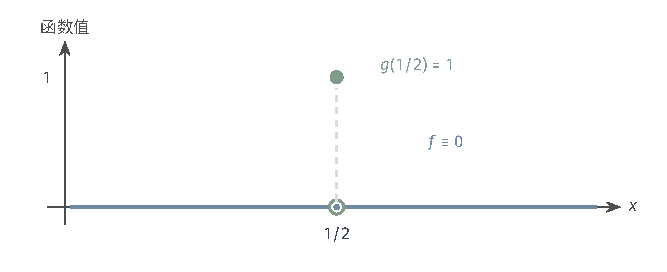
\includegraphics[width=112mm]{figures/00-shared/mathematical-preliminaries-upper/05-space-and-geometry/tikz/comprehension-additions/functional-ae-representatives.pdf}
  \caption{同一积分元素的不同代表。定义域为$[0,1]$并用Lebesgue测度，$f\equiv0$，$g$除$g(1/2)=1$外也为零。绿空心圈表示$g$不在该点取零，圈内蓝点保留$f(1/2)=0$。单点集合测度为零，故任意$1\le p<\infty$下$\|f-g\|_{L^p}=0$；点值读取却不同。}
  \label{fig:vol1-add-functional-ae-representatives}
\end{figure}

\subsubsection{范数、内积与完备性}
\label{subsubsec:norm-inner-product-completeness}

候选及元素相等的含义确定以后，误差公式还必须满足相应公理，极限过程也必须能在同一空间内完成。本节先把范数、Banach条件和Hilbert条件各自要回答的对象与条件说清，后面的具体空间再据此逐一核验。

\paragraph{范数与函数距离}

要比较$f$与$g$的整体偏差，自然的做法是先为单个函数确定“大小”，再由差$f-g$得到两函数之间的距离。在已经确定元素识别的实线性空间$V$上，范数是一个映射$\|\cdot\|:V\to[0,\infty)$，满足三条要求
\begin{align*}
  &\|f\|=0\ \Longleftrightarrow\ f=0,\\
  &\|cf\|=|c|\,\|f\|,\\
  &\|f+g\|\le\|f\|+\|g\|.
\end{align*}
这三条分别保证零误差能被准确识别、按常数缩放时误差一致，以及两段误差合起来不超过各自之和，最后一条就是\term{三角不等式}。令
\[
  d(f,g)=\|f-g\|,
\]
便能把范数公理逐项转成度量公理，从而可以直接回用\BookChapterRef{chap:function-limits}{第~\ref{chap:function-limits}章}关于度量空间中柯西列与完备性的结论。需要强调，如果某个公式在普通函数上只能让非零函数长度为零，就必须先处理这些零方向或改用等价类，不能直接宣布它在原候选上是范数。

同一对函数可以用不同范数衡量：有的强调最大偏差，有的强调积分累计，选哪一种取决于当前真正要控制的误差。这里先建立公理与用途；具体公式是否有限、是否满足三角不等式、能识别何种零元素，分别在下一小节核验。

\paragraph{范数空间的完备性与Banach空间}

对范数空间中的一个柯西列，要区分两件事：“各项彼此越来越接近”与“在候选空间内确实存在一个极限”。若每个范数柯西列都存在$V$中的范数极限，就称$V$为Banach空间。完备性这个条件同时包含所选候选和所选范数，不能只给出一个误差公式就把完备性视为当然。

后面证明具体空间完备时，都会遵循同一条路线：先构造一个候选极限，再证明它保留了该空间的成员条件，最后证明范数误差趋于零。在无限维情形，子空间是否闭、有界列能否抽出范数收敛子列、线性映射是否连续，都必须分别验证，这些性质并不因线性运算成立就自动继承。这里先列清判断边界，后面的投影、读取和算子问题再使用各自的条件。

\paragraph{内积及Hilbert空间}

当任务还要比较函数方向、正交分量或平方误差时，需要在实线性空间上引入内积$\langle f,g\rangle$，要求它对两个变量都是双线性的、对称的，并且$\langle f,f\rangle\ge0$、仅在$f=0$时为零。由
\[
  \|f\|=\sqrt{\langle f,f\rangle}
\]
得到长度。这条长度确实满足三角不等式：对任意实数$t$，
\[
  0\le\|f-tg\|^2=\|f\|^2-2t\langle f,g\rangle+t^2\|g\|^2
\]
是关于$t$的非负二次式，故其判别式不大于零，
\[
  |\langle f,g\rangle|\le\|f\|\|g\|,
\]
即Cauchy--Schwarz不等式；再由
\[
  \|f+g\|^2=\|f\|^2+2\langle f,g\rangle+\|g\|^2
  \le(\|f\|+\|g\|)^2
\]
得到三角不等式。

在这个诱导范数下完备的内积空间称为Hilbert空间，因此Hilbert空间同时也是Banach空间。一般范数未必来自内积，“是否存在内积”与“是否完备”是两个不同的判断。后面的$L^2$、$W^{k,2}$以及正交读取都会注明使用的是哪个内积、完备性从哪里取得。还要提醒一句，内积给出的是函数空间中的正交关系，并不是两条函数图像在平面中相交的几何角度；图~\ref{fig:vol1-add-functional-integral-orthogonality}正好说明这一点。

\begin{figure}[!htb]
  \centering
  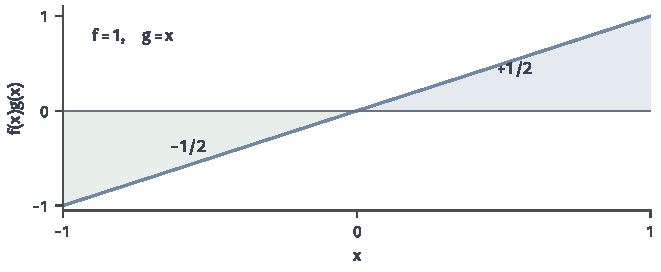
\includegraphics[width=112mm]{figures/00-shared/mathematical-preliminaries-upper/05-space-and-geometry/matplotlib/comprehension-additions/functional-integral-orthogonality.pdf}
  \caption{整函数的正交由内积决定。在$[-1,1]$上用Lebesgue积分内积，取$f(x)=1$、$g(x)=x$。图中曲线是乘积$f(x)g(x)=x$，右侧蓝色区域积分为$1/2$，左侧绿色区域积分为$-1/2$，相加为零。因此两函数正交，所画曲线的平面倾角不承担函数空间夹角的含义。}
  \label{fig:vol1-add-functional-integral-orthogonality}
\end{figure}

\subsection{函数范数的构造}
\label{subsec:constructing-function-norms}

固定一对函数后，按偏差的汇总规则可以分为最大偏差控制和积分累计两类。前者再区分处处控制与允许零测例外的控制，后者固定有限的$p$次累计。每种构造都要说清成员、零元素和极限归属，不把具体空间名称当成互斥类别。

\subsubsection{上确界范数}
\label{subsubsec:supremum-norm}

比较两条曲线时，最大偏差控制要求对允许的全部位置给出一个共同上界。普通函数逐点识别与几乎处处等价类的识别不同，因此一致范数和本质上确界范数要分别构造，不能用一个代表的普通上确界代替等价类的本质上界。

\paragraph{连续函数的一致范数}

固定紧区间$[a,b]$上的实连续函数空间$C([a,b])$。为了同时控制所有位置的偏差，定义
\[
  \|f\|_\infty=\sup_{x\in[a,b]}|f(x)|,\qquad d_\infty(f,g)=\|f-g\|_\infty.
\]
连续性与紧性保证这个上确界有限。范数公理逐条成立：$\|f\|_\infty=0$意味着连续函数$f$在每一点为零，即$f=0$；齐次性由逐点缩放后取上确界直接得到；三角不等式由$|f(x)+g(x)|\le|f(x)|+|g(x)|\le\|f\|_\infty+\|g\|_\infty$对每个$x$成立、再取上确界得到，整个函数便成为范数空间中的一个元素。

取一致范数下的一个柯西列$(f_n)$。固定$x$后，
\[
  |f_n(x)-f_m(x)|\le\|f_n-f_m\|_\infty,
\]
所以右边的标量序列是柯西列，由实数完备性逐点定义$f(x)=\lim_n f_n(x)$。这一步只是构造出候选极限，还没有证明一致收敛或连续性。

一致收敛由共同误差界取得：给定$\varepsilon>0$，取$N$使$n,m\ge N$时$\|f_n-f_m\|_\infty<\varepsilon$；对固定的$x$与$n\ge N$，令$m\to\infty$，由绝对值连续得
\[
  |f_n(x)-f(x)|\le\varepsilon,
\]
该界不依赖$x$，故$\sup_x|f_n(x)-f(x)|\to0$。这一步把逐点构造提升为统一误差控制，是证明极限留在空间内的中间环节。

再固定位置$x_0$，把$|f(x)-f(x_0)|$拆成两端的$f-f_N$误差与中间的$f_N(x)-f_N(x_0)$：先选$N$使两端统一地小于$\varepsilon/3$，再利用$f_N$的连续性选择邻域使中间一项也小于$\varepsilon/3$，三项相加得$|f(x)-f(x_0)|<\varepsilon$，便得到$f$连续。因此极限仍留在$C([a,b])$，与上一步合起来才完成Banach性质的证明。

若输入域不紧，连续函数可能无界，普通上确界便可能为无穷；这时要改选有界连续函数空间或另加增长条件。下一项保持最大偏差的汇总规则，只改变零测例外的约定，而不把输入域不紧的问题误当成本质上界的定义理由。

\paragraph{本质上确界范数}

在测度空间$(X,\mathcal A,\mu)$上，积分任务允许忽略零测集，因此从可测实函数的几乎处处等价类出发，定义
\[
  \|[f]_\mu\|_{L^\infty(\mu)}
  =\inf\{M\ge0:|f|\le M\text{ 在$\mu$下几乎处处成立}\},
\]
以该值有限者构成$L^\infty(\mu)$。\term{本质上确界}不随代表变化：若$g$与$f$几乎处处相等，每个使$|f|\le M$成立的零测例外集与$\{f\neq g\}$取并后仍为零测集，同一$M$也控制$g$；但同一等价类各代表的普通上确界可能差别很大。

范数公理逐项核对。正定性：若$\|f\|_\infty=0$，则对每个正整数$k$都有$|f|\le1/k$几乎处处；这些可测例外集的可数并为零测集，其外$|f|\le1/k$对所有$k$同时成立，故$f=0$几乎处处。齐次性由$|cf|=|c||f|$逐点成立直接得到。三角不等式：若$|f|\le C$在零集$N_f$外成立、$|g|\le D$在零集$N_g$外成立，则在$X\setminus(N_f\cup N_g)$上$|f+g|\le C+D$，例外集仍为零测集，故$\|f+g\|_\infty\le C+D$；对$C,D$各自取下确界，得到$\|f+g\|_\infty\le\|f\|_\infty+\|g\|_\infty$。

完备性证明要小心处理例外集。取$L^\infty$柯西列并选可测代表$f_n$。每项几乎处处有界给出可测零集$N_n^0$，使$|f_n|\le M_n$于$X\setminus N_n^0$；柯西性给出：对每个$n,m$与每个正整数$r$，
\[
  |f_n-f_m|\le\|f_n-f_m\|_\infty+\tfrac1r
\]
几乎处处成立，例外集记为$N_{nmr}$。前章已证明可数个零测集的并仍是零测集，故
\[
  N=\left(\bigcup_n N_n^0\right)\cup\left(\bigcup_{n,m,r\in\mathbb N}N_{nmr}\right)
\]
是单一可测零集。在$X\setminus N$上所有不等式对所有下标同时成立，令$r\to\infty$后，所有需要的差值界便同时成立。不能为每个位置各选一个例外集。

在这个共同补集上，范数柯西性给出了真正的一致柯西性。先固定一项$f_1$的有界控制；柯西列$\{\|f_n-f_1\|_\infty\}$有界，设其上界为$C$，则
\[
  |f_n(x)|\le|f_1(x)|+|f_n(x)-f_1(x)|\le M_1+C,\qquad x\in X\setminus N,
\]
故逐点极限$f(x)=\lim_n f_n(x)$在$X\setminus N$上存在且一致有界；在$N$上补零，并由逐点极限与可测零集改值的可测性，$f$是可测代表且$f\in L^\infty$。把共同柯西界的一端送到极限：对$x\in X\setminus N$，
\[
  |f_n(x)-f(x)|=\lim_{m\to\infty}|f_n(x)-f_m(x)|
  \le\limsup_{m\to\infty}\|f_n-f_m\|_\infty,
\]
这在零集$N$之外成立，故$\|f_n-f\|_\infty\le\limsup_m\|f_n-f_m\|_\infty\to0$。于是得到本质上确界范数收敛以及极限的有限本质上界，从而证明$L^\infty$完备。零测修改不改变元素，仍不回答某一指定点值是否确定——这项读取问题要交给后面的点值良定义性处理。

\subsubsection{积分范数}
\label{subsubsec:integral-norms}

若总体偏差按测度累计，就要先选定$p$次累计以及有限积分的成员，再证明范数性质和完备性。下列三个有标题的单元分别负责对象构造、误差公理和空间内极限，不把证明中的每个临时步骤另升成标题。

\paragraph{$L^p$空间及其范数}

固定测度空间与$1\le p<\infty$，从满足
\[
  \int_X|f|^p\,\mathrm d\mu<\infty
\]
的可测实函数出发，按几乎处处相等取等价类。以这些等价类组成$L^p(\mu)$；零积分差识别的是同一等价类，而不是每个位置的值都相同。为了使整体缩放$f\mapsto cf$对应误差乘$|c|$，定义
\[
  \|[f]\|_p=\left(\int_X|f|^p\,\mathrm d\mu\right)^{1/p},
\]
并核对换代表不改变数值：前章已证明零测集上的改动不改变勒贝格积分。$p=1$累计绝对偏差，$p=2$累计平方偏差后开方，一般的$p$改变对大偏差的计价，公式的用途先于不等式证明说明。下文常用代表元$f$代写等价类$[f]$，并简记范数为$\|f\|_p$。

在$[0,1]$的Lebesgue测度下取$f_n(x)=x^n$，可算得
\[
  \|f_n\|_p=\left(\int_0^1x^{np}\,\mathrm dx\right)^{1/p}
  =\left(\frac{1}{np+1}\right)^{1/p}.
\]
它的逐点极限在$x<1$时为零、在$x=1$时为一，仍代表零积分元素；而普通一致范数恒为一。这个例子同时区分了普通函数极限、积分等价类和最大偏差，后面比较各种收敛时只回用这里的计算结果。

现有公式还没有自动保证三角不等式与空间完备性。先用
\[
  |f+g|^p\le 2^{p-1}(|f|^p+|g|^p)
\]
说明成员对加法封闭：逐点有
\[
  (a+b)^p\le(2\max\{a,b\})^p=2^p\max\{a^p,b^p\}\le2^{p-1}(a^p+b^p),
\]
积分后即知$f,g\in L^p$时$f+g\in L^p$。有限$p$与前面的$L^\infty$构造始终保持各自条件。

\paragraph{Hölder不等式与范数性质}

对$1<p<\infty$固定共轭指数$q=p/(p-1)$，则$1/p+1/q=1$。先证明标量Young不等式：对$a,b\ge0$，
\[
  ab\le\frac{a^p}{p}+\frac{b^q}{q}.
\]
固定$b\ge0$，考虑关于$s\ge0$的函数$F(s)=s^p/p-bs$。其导数$s^{p-1}-b$在$s_*=b^{1/(p-1)}=b^{q/p}$处为零，且$F''(s)=(p-1)s^{p-2}>0$，故该处取最小值；代入得$F(s_*)=-b^q/q$，于是$F(s)\ge-b^q/q$对所有$s\ge0$成立，取$s=a$即得Young不等式。

对非零且有限范数的函数，在Young不等式中取
\[
  a=\frac{|f|}{\|f\|_p},\qquad b=\frac{|g|}{\|g\|_q},
\]
积分并复用前章积分的线性与单调性，得到
\[
  \frac{1}{\|f\|_p\|g\|_q}\int_X|fg|\,\mathrm d\mu
  \le\frac{1}{p\|f\|_p^p}\int_X|f|^p\,\mathrm d\mu
  +\frac{1}{q\|g\|_q^q}\int_X|g|^q\,\mathrm d\mu
  =\frac1p+\frac1q=1,
\]
再恢复尺度，得到Hölder不等式
\[
  \int_X|fg|\,\mathrm d\mu\le\|f\|_p\|g\|_q.
\]
若$\|f\|_p=0$，由前章零积分判别定理（$\int|f|=0$当且仅当$f=0$几乎处处）知$fg=0$几乎处处，不等式为平凡$0\le0$；端点$L^1$与$L^\infty$的配对直接由$|fg|\le|f|\|g\|_\infty$积分估计。

已知$f+g\in L^p$后，\term{Minkowski不等式}按如下推导。先由$|f+g|^p=|f+g|^{p-1}|f+g|\le|f+g|^{p-1}(|f|+|g|)$，把$\int|f+g|^p$写成
\[
  \int_X|f+g|^{p-1}|f|\,\mathrm d\mu
  +\int_X|f+g|^{p-1}|g|\,\mathrm d\mu.
\]
两项分别对$|f+g|^{p-1}$与$|f|$、$|g|$应用Hölder。由$(p-1)q=p$，
\[
\begin{aligned}
  \int_X|f+g|^{p-1}|f|\,\mathrm d\mu
  &\le\left(\int_X|f+g|^{(p-1)q}\,\mathrm d\mu\right)^{1/q}\|f\|_p\\
  &=\left(\int_X|f+g|^p\,\mathrm d\mu\right)^{1/q}\|f\|_p,
\end{aligned}
\]
第二项同理，合并得
\[
  \int_X|f+g|^p\,\mathrm d\mu
  \le\left(\int_X|f+g|^p\,\mathrm d\mu\right)^{1/q}
  \bigl(\|f\|_p+\|g\|_p\bigr).
\]
若$\|f+g\|_p>0$，两端同除$(\int|f+g|^p)^{1/q}$，利用$p-p/q=p(1-1/q)=p/p=1$，便得到\term{Minkowski不等式}
\[
  \|f+g\|_p\le\|f\|_p+\|g\|_p.
\]
若$\|f+g\|_p=0$，$f+g$为零等价类，不等式平凡成立。零值情形必须单独落下，不能略过约去项所需的条件。$p=1$时直接对绝对值的逐点三角不等式积分，与前两段合起来完成所有有限$1\le p<\infty$的范数性质。两点计数测度下取两个不相交的单位向量可以看出范围$p\ge1$的实际作用：当$0<p<1$时，两者之和的$p$次累计根为$2^{1/p}>2$，同一公式在该范围不满足范数\term{三角不等式}。

对$p=2$给出
\[
  \langle f,g\rangle=\int_Xfg\,\mathrm d\mu,
\]
由Hölder保证积分存在，逐项核对它是实内积并识别其诱导范数。此时只得到内积结构；等下一单元的完备性完成后，才能据此称$L^2$为Hilbert空间。

\paragraph{$L^p$空间的完备性}

对$L^p$柯西列$(f_n)$，依次选取子列$(f_{n_k})$使
\[
  \sum_k\|f_{n_{k+1}}-f_{n_k}\|_p<\infty.
\]
之所以能选出这样“快速缩小相邻差”的子列，是柯西条件的直接推论：递归取$n_k$，使$n,m\ge n_k$时$\|f_n-f_m\|_p<2^{-k}$。选好子列后再取可测代表，不能把整个原列的逐点收敛当成前提。

对有限部分和
\[
  S_m=|f_{n_1}|+\sum_{k=1}^{m}|f_{n_{k+1}}-f_{n_k}|
\]
使用Minkowski不等式，得到与$m$无关的有限范数上界：
\[
  \|S_m\|_p\le\|f_{n_1}\|_p+\sum_{k=1}^m\|f_{n_{k+1}}-f_{n_k}\|_p\le C.
\]
数列$S_m$逐点单调不减，故$S_m^p\uparrow S^p$。由前章的单调收敛定理，
\[
  \int_XS^p\,\mathrm d\mu=\lim_{m\to\infty}\int_XS_m^p\,\mathrm d\mu\le C^p<\infty,
\]
取得$S=\lim_mS_m\in L^p$，故$S<\infty$几乎处处。这一步补出了“无穷差分累计仍可被积分控制”的依据。

在$S$有限处，差分级数$\sum_k(f_{n_{k+1}}-f_{n_k})$被$S$控制而绝对收敛，定义
\[
  f=f_{n_1}+\sum_k(f_{n_{k+1}}-f_{n_k}),
\]
并在可测零例外集$\{S=\infty\}$上置零。由逐点极限的可测性以及$|f|\le S$，得到可测代表及有限的$p$次积分，确认候选极限属于原来的$L^p$空间。

再用同样的有限和估计控制尾和：对部分和$T_{j,m}=\sum_{k=j}^m(f_{n_{k+1}}-f_{n_k})$，Minkowski给$\|T_{j,m}\|_p\le\sum_{k=j}^m\|f_{n_{k+1}}-f_{n_k}\|_p$；$m\to\infty$时$T_{j,m}\to f-f_{n_j}$几乎处处，由前章Fatou引理，
\[
\begin{aligned}
  \|f-f_{n_j}\|_p^p
  &=\int\liminf_m|T_{j,m}|^p\,\mathrm d\mu\\
  &\le\liminf_m\int|T_{j,m}|^p\,\mathrm d\mu\\
  &\le\left(\sum_{k\ge j}\|f_{n_{k+1}}-f_{n_k}\|_p\right)^p,
\end{aligned}
\]
得到
\[
  \|f-f_{n_j}\|_p\le\sum_{k\ge j}\|f_{n_{k+1}}-f_{n_k}\|_p\to0.
\]
最后把$\|f_n-f\|_p$拆成“原列到某个固定子列项的柯西误差”与“该子列项到$f$的误差”：先取$j$足够小使第二项小，再用柯西性取$n,n_j$足够接近使第一项小，便取得整列收敛；只构造出子列极限尚不足以得到这一结论。汇合成员资格、范数收敛和前面的内积结构可知：所有$1\le p<\infty$的$L^p$都是Banach空间，$L^2$进一步是Hilbert空间。与本质上确界范数的单独证明相对照，这里明确没有把$p=\infty$混入有限$p$的累计公式。

\subsection{函数空间与误差的比较}
\label{subsec:comparing-spaces-errors}

具体空间建立以后，本节分别问三件事：成员能否转入另一空间，更换测度后是否仍识别相同元素，以及不同误差趋零能推出哪些结论。三个问题各有对象和条件，先处理成员与零集，再用定量不等式比较误差；包含关系本身不替代范数比较。

\subsubsection{函数空间的包含关系}
\label{subsubsec:inclusion-relations}

同一个普通函数满足较强条件时，可能合法地成为另一空间的元素；但进入等价类空间时，要说清这里的“包含”究竟是集合包含还是自然映射。

固定输入域与连续生成函数$\varphi_1,\ldots,\varphi_m$，由连续性对有限线性组合封闭，得到
\[
  \operatorname{span}\{\varphi_j\}\subset C(X).
\]
这是真正的普通函数集合包含，不需要先取几乎处处等价类。

对同一测度且$0<\mu(X)<\infty$、$1\le p<q<\infty$，把已证明的Hölder用于$|f|^p\cdot1$，使用共轭指数$q/p$与$q/(q-p)$，得到
\[
  \int_X|f|^p\,\mathrm d\mu
  \le\left(\int_X|f|^{q}\,\mathrm d\mu\right)^{p/q}
  \left(\int_X1^{q/(q-p)}\,\mathrm d\mu\right)^{(q-p)/q}
  =\|f\|_q^p\,\mu(X)^{(q-p)/q},
\]
两端开$p$次方，即
\begin{equation}
  \|f\|_p\le\mu(X)^{1/p-1/q}\|f\|_q.
  \label{eq:functional-lp-inclusion}
\end{equation}
右端有限才推出$L^q\subseteq L^p$；$q=\infty$时由本质上界积分另得相同形式的端点估计：$\int_X|f|^p\,\mathrm d\mu\le\|f\|_\infty^p\mu(X)$，开$p$次方得$\|f\|_p\le\mu(X)^{1/p}\|f\|_\infty$，不重复Hölder证明。

紧域上的连续函数有界，有限Borel测度由此保证其有限$p$次积分的成员资格。把普通函数送入积分空间时要明确写成$f\mapsto[f]_\mu$；若测度不是全支撑，不同的连续函数仍可能代表同一元素，因此这是自然映射，只有在核实单射条件后才能把它当作函数空间嵌入。

无限总测度下，式~\eqref{eq:functional-lp-inclusion}中的质量常数不再给出有限控制。例如无限Lebesgue测度上的常数一属于$L^\infty$，却不属于任何有限$p$的$L^p$。这就界定了包含结论的范围。同一测度下成员关系清楚以后，下一题保持函数不变，转向改变计价测度会发生什么。

\subsubsection{换测度后的元素与范数}
\label{subsubsec:change-of-measure}

在同一可测集合上改用另一测度，首先可能改变的是“哪些差异完全不计价”，随后才是误差大小的改变。测度间的零集关系在此本地固定：对两个测度$\mu,\nu$，若每个$\mu$零测集也是$\nu$零测集，称$\nu$关于$\mu$\term{绝对连续}，记作$\nu\ll\mu$；若$\mu\ll\nu$与$\nu\ll\mu$同时成立，两测度有完全相同的零集，称为相互绝对连续（等价测度）。下面把这些关系落实到函数元素和范数上。

\paragraph{零集关系与等价类识别}

固定共同可测空间上的$\mu,\nu$，回用$f\sim_\mu g$当且仅当$f=g$在$\mu$下几乎处处。若$\nu\ll\mu$，则$\mu$零测的差异也是$\nu$零测的，因而映射$[f]_\mu\mapsto[f]_\nu$在可测函数的等价类层面不依赖代表。这个结论并没有自动保证一个$L^p(\mu)$成员还具有有限的$\nu$积分。

如果两测度相互绝对连续，它们识别相同的零差异；若只在一个方向绝对连续，新测度可能把更多函数归为同一元素。以$[0,1]$上$\mathrm d\nu=w\,\mathrm d\mu$为例：这里$\nu(B)=\int_Bw\,\mathrm d\mu$是一个测度，其可数可加性由前章非负函数项级数的逐项积分定理保证，且它自动满足$\nu\ll\mu$。令$w$在一块原本正测度的区域上为零，那么两个只在该区域不同的函数，可由不同的$\mu$类合成同一个$\nu$类。这里要把相互绝对连续（等价测度）与“相等测度”区分开：$\mu$与$2\mu$有相同的零集，却是不同的测度。另外，“任意$\nu\ll\mu$都有形如$\mathrm d\nu=w\,\mathrm d\mu$的密度”这一反方向结论是Radon--Nikodym定理，其一般证明见教材\scite{math-folland1999real}，本节只使用直接给出的加权测度，不把该定理当作本地已证结论。

即使$w>0$几乎处处、零集识别相同，若$w$没有统一上界或正下界，也不能据此给出两个范数之间统一的比较常数。这里先把元素识别与定量大小分开，正说明下一单元增加密度界的必要性；指定点值的读取仍留到点值读取一节处理。

\paragraph{密度界与范数换算}

在$\mathrm d\nu=w\,\mathrm d\mu$及有限$1\le p<\infty$下，把差函数$h=f-g$代入相对密度的积分公式，先写
\[
  \|h\|_{L^p(\nu)}^p=\int_X|h|^pw\,\mathrm d\mu.
\]
若$w\le C<\infty$几乎处处，便由积分单调性逐步得到
\[
  \|h\|_{L^p(\nu)}^p\le C\int_X|h|^p\,\mathrm d\mu=C\|h\|_{L^p(\mu)}^p,
\qquad
  \|h\|_{L^p(\nu)}\le C^{1/p}\|h\|_{L^p(\mu)}.
\]
同一估计同时保证了从$L^p(\mu)$到$L^p(\nu)$的成员转换，这一点不能从绝对连续单独推出。

若再有$0<c\le w$几乎处处，反向得到
\[
  c^{1/p}\|h\|_{L^p(\mu)}\le\|h\|_{L^p(\nu)},
\]
从而两边成员资格一致，误差由双向常数控制。$L^\infty$另外依赖零集识别：等价测度给出相同的本质上确界，不能给它硬套有限$p$的$C^{1/p}$推导；只有单向绝对连续时，只能得到相应方向的本质上界控制。回头看例子可知，比较时必须同时注明测度、指数以及密度上下界。前两段处理的是同一差函数在两种计价规则中的大小，尚未涉及一列函数如何趋近；下一题就在这些量化控制上建立收敛蕴含。

\subsubsection{函数距离与收敛方式的比较}
\label{subsubsec:convergence-comparison}

固定候选、元素识别和误差以后，“误差趋零”才有具体含义。本单元共同定义范数收敛、逐点收敛和一致收敛，并用不同范数与同一序列检验蕴含关系；后面的计算迭代、截断和正则化解族只复用这些判断，不重新定义。

\paragraph{范数、逐点与一致收敛}

固定范数空间中的候选极限$f$，定义$f_n\to f$为$\|f_n-f\|\to0$，并写清这个范数及其测度。若空间元素是几乎处处等价类，所比较的是类的误差，不能不选代表就把它解释成每点函数值都收敛。

对同一输入集合上的普通函数，逐点收敛要求对每个固定的$x$都有$f_n(x)\to f(x)$，但允许所需序号随$x$而变。一致收敛则要求：对每个$\varepsilon>0$，存在一个统一的$N$，使所有$n\ge N$和所有$x$都满足
\[
  |f_n(x)-f(x)|<\varepsilon.
\]
共同阈值解释了为什么一致控制强于逐点控制。

用前面$x^n$的计算结果比较：它在$[0,1]$上逐点趋于一条“端点为一、其余为零”的函数，有限$p$范数趋零，却没有一致地趋于该逐点极限。三个陈述分别使用普通函数极限、积分零元素和统一偏差，并不相互矛盾。

\paragraph{范数比较与收敛蕴含}

对同一对函数的差$h=f-g$，若已经取得
\[
  \|h\|_A\le C\|h\|_B
\]
且$C$不随函数序号改变，那么$B$范数误差趋零才能传成$A$范数误差趋零。双向常数控制给出两种范数收敛等价；“同一函数集合”或各自范数有限都不能替代这项统一估计。

回用有限测度包含中的估计，得到$L^q$收敛推出$L^p$收敛；回用
\[
  \|h\|_p\le\mu(X)^{1/p}\|h\|_\infty,
\]
得到有限总测度下一致误差趋零推出$L^p$误差趋零。这里是从已建立的常数转为序列结论，不再重做Hölder证明。

改成实轴上的无限Lebesgue测度，取
\[
  h_n=\tfrac1n\,\mathbb I_{[0,n^2]}.
\]
直接算得普通上确界为$1/n\to0$，而
\[
  \|h_n\|_2^2=\frac{1}{n^2}\cdot n^2=1;
\]
支撑范围同时扩大使有限测度结论失效，不能只看函数高度判断积分误差。更换测度后的收敛蕴含同样使用上一题的密度界，并保留其方向和常数。无论更换$p$、测度还是最大偏差规则，都要先给定同一差函数的定量控制，再谈误差极限；由范数到具体读数还要检验相应读取的有界性，这项新增问题由点值读取的有界性展开，不在此复述连续尖峰证明。

\paragraph{逐点判断与积分误差的边界}

为检验$L^p$收敛能否自动控制整列的每点行为，在$[0,1)$上按层排列二进区间指示函数：第$k$层依次取
\[
  [j2^{-k},(j+1)2^{-k}),\qquad j=0,\ldots,2^k-1,
\]
再按层展开成一个序列。每项的$L^p$范数为
\[
  \|h_{k,j}\|_p=\left(\int_{j2^{-k}}^{(j+1)2^{-k}}1\,\mathrm dx\right)^{1/p}=2^{-k/p},
\]
随序号增长而趋零。但对每个固定的$x\in[0,1)$，每一层恰有一项在该点取一，而充分大的层里也有其他项取零。因此整列在该点反复出现零和一，不逐点收敛；这是真正的同一列代表函数行为，不是任意更改零测点造成的现象，也不排除另选子列的结论。

反方向固定$[0,1]$上的Lebesgue测度，取$g_n=n\,\mathbb I_{(0,1/n)}$。每个位置最终都落在支撑外，所以$g_n$处处趋零，而
\[
  \|g_n\|_2^2=n;
\]
逐点阈值随位置变化并允许窄区间上的峰值增长，不能单独控制积分误差。若要由逐点或几乎处处极限转移积分，必须另给支配等条件并回用前章的支配收敛定理。

\paragraph{系数距离与函数距离}

对$[-1,1]$及$\mathrm d\mu=\mathrm dt/2$，固定仿射表示$f(t)=a+bt$。把两个函数之差$\delta a+\delta bt$平方积分，交叉项因对称区间上$t$的积分为零，得到
\[
  \|\delta a+\delta bt\|_{L^2}^2=(\delta a)^2+\frac{(\delta b)^2}{3},
\]
而原系数的欧氏距离平方为$(\delta a)^2+(\delta b)^2$。这个差异来源于基函数在当前内积下的尺度，可概括为有限表示的函数误差二次型
\[
  \delta c^{\top}G\,\delta c,\qquad G_{ij}=\langle\varphi_i,\varphi_j\rangle.
\]
改变基必须连同系数和\term{Gram矩阵}一起变换；这里比较的是既定表示下的两种误差，记录转换与冗余方向的完整讨论由后面的系数与读数转换承接。

\section{弱导数与Sobolev空间}
\label{sec:weak-derivatives-sobolev}

绝对值函数在尖点没有经典导数，但把导数转移给光滑测试函数以后，积分恒等式仍然能够表达它的变化。本节先建立测试函数与分布的共同配对，再判断分布导数何时能由普通函数表示，最后把函数及规定阶弱导的积分控制组织成Sobolev空间。点值和边界迹属于随后读取任务的内容。

\subsection{测试函数与分布}
\label{subsec:test-functions-distributions}

把导数转移到测试函数之前，必须说明测试函数是什么、为什么能避开边界，以及什么对象可以与它配对。两个子题分别建立接收测试的空间和作用于测试的连续线性泛函，给出弱导定义的共同对象。

\subsubsection{紧支撑测试与局部可积函数}
\label{subsubsec:test-functions-local-integrable}

固定非空开域$\Omega\subset\mathbb R^d$，取光滑且支撑紧含于$\Omega$的函数$\varphi\in C_c^\infty(\Omega)$。可以先在内部一块区域上想象一个光滑凸起：函数在靠近域边界之前就已经恒为零，因此分部积分时不会留下边界项。把这样的光滑凸起归一化到积分为一，还能为后面的局部平滑做准备。

定义$f\in L^1_{\mathrm{loc}}(\Omega)$表示：在每个紧子集$K\Subset\Omega$上，$|f|$的积分都有限。测试函数有界且只占一块紧支撑，因此
\[
  \int_\Omega f\varphi\,\mathrm dx
\]
有限。这说明不需要先要求$f$在整个域上可积，也能合法地形成局部测试配对。

为了把“连续作用”与任意代数线性作用区分开，还要说明测试函数序列趋零的条件：它们的全部支撑落在同一个紧集内，并且每个阶数的导数都一致趋零。支撑共同受限和各阶控制这两条都不能省；下一题正是用这种收敛说明分布的连续性，而不把测试空间误当成只带一个上确界范数的空间。

\subsubsection{分布及普通函数的表示}
\label{subsubsec:distributions-regular}

\paragraph{分布的定义}

“给每个测试函数一个线性读数”自然引出分布：分布$T$就是测试函数空间上的连续线性泛函。连续性可以写成本地可核对的估计：对每个紧集$K\Subset\Omega$，存在常数$C_K$和有限整数$m_K$，使支撑在$K$内的测试满足
\[
  |T(\varphi)|\le C_K\max_{|\alpha|\le m_K}\sup|D^\alpha\varphi|.
\]
这里的多重指标$\alpha=(\alpha_1,\ldots,\alpha_d)$是一组非负整数，$|\alpha|=\alpha_1+\cdots+\alpha_d$是总阶数，$D^\alpha\varphi=\partial_1^{\alpha_1}\cdots\partial_d^{\alpha_d}\varphi$是对应偏导。

这个估计说明：上一题那种“共同紧支撑、各阶导数一致趋零”的测试序列趋零时，读数$T(\varphi)$也趋零。因此分布保留了对光滑测试变化的连续响应，而任意代数线性映射并不自动满足这一点。本节只使用这一本地连续性，不展开完整的局部凸拓扑理论。

\paragraph{局部可积函数与Dirac分布}

对$f\in L^1_{\mathrm{loc}}$定义
\[
  T_f(\varphi)=\int_\Omega f\varphi\,\mathrm dx,
\]
由
\[
  |T_f(\varphi)|\le\left(\int_K|f|\,\mathrm dx\right)\sup_K|\varphi|
\]
即可核对线性和连续性。称这类分布由普通函数表示；换成几乎处处相同的$f$不改变分布。要注意，它输出读数的对象是光滑测试，而不是任意函数在某一点的值。

另取$x_0\in\Omega$，以
\[
  \delta_{x_0}(\varphi)=\varphi(x_0)
\]
定义Dirac分布。上确界控制即可证明其连续性，因而它也是合法分布。这与上一段并列说明：分布接收测试的方式不必都是对某个局部可积密度做积分。这一区别为后面阶跃函数导数的输出预留了正确类型。

\subsection{分布导数与普通弱导数}
\label{subsec:distribution-weak-derivatives}

分布提供了统一配对以后，本小节先把经典分部积分改写成分布导数，再单独判断导数是否具有局部可积函数表示。普通弱导是“表示条件成立”的情形，不与分布导数列成互不相干的两套微分。

\subsubsection{将导数转移到测试函数}
\label{subsubsec:transfer-derivative}

对经典光滑$f$和$\varphi\in C_c^\infty(\Omega)$逐次分部积分，可写
\[
  \int_\Omega (D^\alpha f)\varphi\,\mathrm dx
  =(-1)^{|\alpha|}\int_\Omega fD^\alpha\varphi\,\mathrm dx.
\]
每转移一次导数产生一个负号，紧支撑消去了边界项。等式右边只要求$f$能与光滑测试的导数配对，这就为尖点情形提供了仍可使用的形式。

据此对任意分布$T$定义
\[
  D^\alpha T(\varphi)=(-1)^{|\alpha|}T(D^\alpha\varphi).
\]
导数保持测试函数的共同紧支撑，并把有限阶导数控制变成更高有限阶的控制，因此新作用仍是连续线性泛函；这才保证分布导数始终作为分布存在。

若输入本来是光滑函数所表示的$T_f$，第一段恒等式给出$D^\alpha T_f=T_{D^\alpha f}$，新定义因而与经典导数兼容。一般分布的输出尚未承诺有普通函数表示，下一题专门增加这一条件，而不从“分布导数存在”跳到“普通弱导一定存在”。

\subsubsection{普通弱导数的存在与唯一性}
\label{subsubsec:weak-derivative-existence-uniqueness}

\paragraph{局部可积表示与弱导数}

固定$f\in L^1_{\mathrm{loc}}(\Omega)$。若存在$g\in L^1_{\mathrm{loc}}(\Omega)$，使所有测试函数都满足
\begin{equation}
  \int_\Omega g\varphi\,\mathrm dx
  =(-1)^{|\alpha|}\int_\Omega fD^\alpha\varphi\,\mathrm dx,
  \label{eq:functional-weak-derivative}
\end{equation}
便称$g$为$f$的$\alpha$阶普通\term{弱导数}，记$D^\alpha f=g$。用分布语言说就是$D^\alpha T_f=T_g$；与上一题相比，“存在局部可积函数$g$表示这个分布导数”是新增条件。弱导恒等式必须对所有测试成立，不能只在少数几个探测函数上核对，也不能用“经典导数几乎处处存在”代替它。输入和输出都以几乎处处等价类识别，换代表不改变恒等式。

\paragraph{弱导数的几乎处处唯一性}

若$g_1,g_2$都满足同一个弱导恒等式，相减得到$h=g_1-g_2\in L^1_{\mathrm{loc}}(\Omega)$，对所有紧支撑光滑测试的积分为零。要从这组测试信息恢复$h$，先证明两个本地引理。

第一，卷积的$L^1$控制。取非负光滑凸起$\rho$支撑在单位球、积分为一，令
\[
  \rho_\varepsilon(x)=\varepsilon^{-d}\rho(x/\varepsilon),
\]
则$\rho_\varepsilon$仍非负、积分为一、支撑在$B(0,\varepsilon)$内。对任意$u\in L^1$，
\[
\begin{aligned}
  \|u*\rho_\varepsilon\|_1
  &=\int\left|\int u(y)\rho_\varepsilon(x-y)\,\mathrm dy\right|\mathrm dx\\
  &\le\int\int|u(y)|\rho_\varepsilon(x-y)\,\mathrm dx\mathrm dy\\
  &=\|u\|_1,
\end{aligned}
\]
最后一步对非负被积函数交换累次积分，依据前章单调收敛建立的非负积分交换次序结论，且内层积分$\int\rho_\varepsilon(x-y)\,\mathrm dx=1$。

第二，近似恒等的恢复。对紧集$K\Subset\Omega$，要证明$\|h*\rho_\varepsilon-h\|_{L^1(K)}\to0$。先看$h$为紧支撑连续函数的情形：一致连续性给出$\sup_{|z|<\varepsilon}\|h(\cdot-z)-h\|_1\to0$，而
\[
  (h*\rho_\varepsilon)(x)-h(x)=\int[h(x-z)-h(x)]\rho_\varepsilon(z)\,\mathrm dz,
\]
积分后用$\rho_\varepsilon$质量为一控制，即得上式趋零。对一般$h\in L^1$，先用紧支撑连续函数$g$在$L^1$中逼近（该稠密性是标准结论，见教材\scite{math-folland1999real}），再由三角不等式与第一条引理，
\[
\begin{aligned}
  \|h*\rho_\varepsilon-h\|_1
  &\le\|(h-g)*\rho_\varepsilon\|_1+\|g*\rho_\varepsilon-g\|_1+\|g-h\|_1\\
  &\le2\|h-g\|_1+\|g*\rho_\varepsilon-g\|_1,
\end{aligned}
\]
先把$\|h-g\|_1$取得任意小，再令$\varepsilon\to0$，恢复成立。这就是题目所说的“局部$L^1$平移连续性”：先对紧支撑连续函数用一致连续性证明，再经局部$L^1$逼近传给$h$，不能只把“平滑后恢复”当成名称。

回到$h$。对每个使$B(x,\varepsilon)\subset\Omega$的允许中心$x$，函数$y\mapsto\rho_\varepsilon(x-y)$是合法测试，故
\[
  h*\rho_\varepsilon(x)=0.
\]
在近似恒等恢复中令$\varepsilon\to0$，得$\|h\|_{L^1(K)}=0$对每个紧$K\Subset\Omega$成立；由前章零积分判别定理，$h=0$几乎处处于$K$。再取可数个紧集
\[
  K_j=\{x\in\Omega:|x|\le j,\ \operatorname{dist}(x,\partial\Omega)\ge1/j\}
\]
覆盖$\Omega$，把零例外集取可数并，便得到$h=0$几乎处处于$\Omega$的全域结论。因此弱导唯一的是等价类，某个零测点上的取值仍可不同。

\subsubsection{尖点与跳跃的不同输出}
\label{subsubsec:cusp-jump-outputs}

对实轴上的$f(x)=|x|$，在零点左右分别分部积分，零点处函数值为零使边界项相接，得到
\[
  \int_{\mathbb R}|x|\varphi'(x)\,\mathrm dx
  =-\int_{\mathbb R}\operatorname{sgn}(x)\,\varphi(x)\,\mathrm dx,
\]
即$Df=\operatorname{sgn}x$的弱导恒等式成立。原函数在零点不具经典导数，却仍有局部可积的一阶弱导；$\operatorname{sgn}0$如何约定不影响输出等价类。

改取阶跃$H(x)=\mathbb I_{(0,\infty)}(x)$，计算
\[
  -\int_{\mathbb R}H\varphi'\,\mathrm dx
  =-\int_0^\infty\varphi'\,\mathrm dx
  =\varphi(0),
\]
得到分布导数$DH=\delta_0$。这里跳跃留下的是测试在跳点的取值，输出类型已不同于前一例的普通函数。

事实上，假设$\delta_0=T_g$且$g\in L^1_{\mathrm{loc}}$，取一列零点值为一、绝对值至多一、支撑缩向零点的光滑测试$\varphi_\varepsilon$。由前章对小测度集合上积分的估计（积分的绝对连续性），$\int g\varphi_\varepsilon\,\mathrm dx\to0$，而$\delta_0(\varphi_\varepsilon)=1$，矛盾。因此阶跃的分布导数不能由局部可积函数表示。两例放在一起，正好标出“表示条件”成立与否的边界，接下来便把普通弱导的大小控制交给Sobolev空间。

图~\ref{fig:functional-weak-derivative}把这两条函数并列：弱导数允许用一个几乎处处确定的函数保存变化信息，而不要求补出尖点处不存在的经典导数。
\begin{fullwidth}
\begin{minipage}{\linewidth}
 \centering
 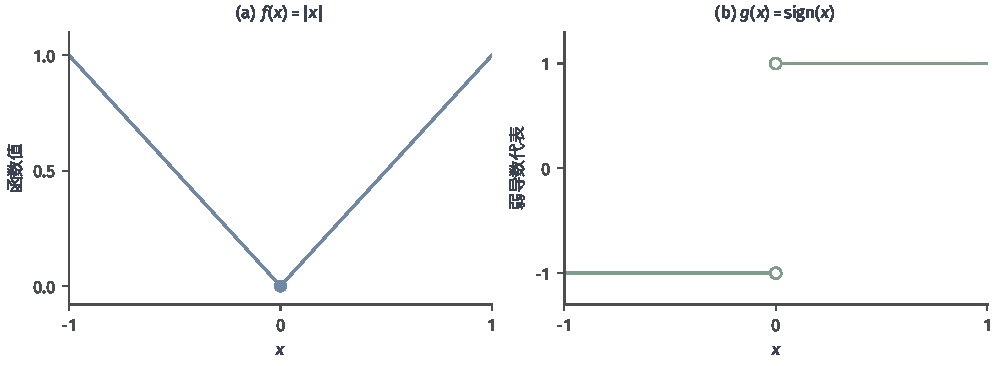
\includegraphics[width=169mm]{figures/00-shared/mathematical-preliminaries-upper/05-space-and-geometry/matplotlib/concepts-analysis-functional/weak-derivative.pdf}
 \functionalinlinefigurecaption{fig:functional-weak-derivative}
   {$f(x)=|x|$与其一阶弱导数$g(x)=\operatorname{sgn}(x)$。左图原点为连续尖点；右图两段分别为$-1$与$1$，空心端点表示经典导数在原点未定义。弱导数在原点的代表值可以任取，积分恒等式不受影响。}
\end{minipage}
\end{fullwidth}

\subsection{Sobolev空间}
\label{subsec:sobolev-spaces}

普通弱导存在还没有控制函数及导数的整体大小。本小节把规定阶弱导与原函数一起纳入范数，先确定成员与微分的定义域，再证明极限中的导数仍属于同一个函数；$p=2$的内积结构与$p=\infty$的补充范围分别标明。

\subsubsection{函数与弱导的共同积分控制}
\label{subsubsec:sobolev-members-norm}

\paragraph{$W^{k,p}$的成员与范数}

固定开域$\Omega\subset\mathbb R^d$、整数$k\ge0$及$1\le p<\infty$。为了同时控制函数偏差与规定阶的变化量，定义$W^{k,p}(\Omega)$由这样的$u$构成：
\[
  u\in L^p(\Omega),\qquad D^\alpha u\in L^p(\Omega)\quad(|\alpha|\le k),
\]
其中$D^0u=u$。局部可积性由$L^p$在紧集上的Hölder控制取得，因此这些弱导恒等式都有意义。

在这些等价类上定义
\begin{equation}
  \|u\|_{W^{k,p}}
  =\left(\sum_{|\alpha|\le k}\|D^\alpha u\|_p^p\right)^{1/p}.
  \label{eq:functional-sobolev-norm}
\end{equation}
零阶项控制函数本身，其余项控制各规定阶的变化量。有限个$L^p$分量的线性、正定与Minkowski不等式保证这是一个范数；只累计某一阶导数通常无法区分常数等零方向，不能不另作处理就替代当前全范数。

在有限区间$(-1,1)$上回用绝对值的弱导计算：函数和符号函数都属于每个有限$p$的$L^p$，故$|x|\in W^{1,p}(-1,1)$。阶跃虽属于该区间的$L^p$，但它的一阶分布导数是Dirac、没有普通局部可积表示，因此不属于$W^{1,p}$。这里用成员判定承接前例，不重复分部积分过程。

\paragraph{弱微分的定义域与误差控制}

对$|\alpha|\le k$，把弱微分看成映射
\[
  D^\alpha:W^{k,p}(\Omega)\to L^p(\Omega),
\]
由范数中包含该项直接得到
\[
  \|D^\alpha u\|_p\le\|u\|_{W^{k,p}}.
\]
相减后同样得到$\|D^\alpha(u-v)\|_p\le\|u-v\|_{W^{k,p}}$，因此这是在指定输入范数和定义域下的有界线性操作。

但这项控制不能被改写成“微分在任意$L^p\to L^p$上都有界”：普通$L^p$成员未必有该阶弱导，即使有导数，也没有这里的共同范数控制。输出仍是体内的弱导等价类，域内点值与整条边界记录要由后面的点值与边界读取按其输出类型另建条件。

\subsubsection{Sobolev空间的完备性}
\label{subsubsec:sobolev-completeness}

\paragraph{分量极限与弱导恒等式}

取$W^{k,p}$柯西列$(u_n)$。因为每一分量范数都不超过全范数，
\[
  \|D^\alpha u_n-D^\alpha u_m\|_p\le\|u_n-u_m\|_{W^{k,p}},
\]
故$(D^\alpha u_n)$对每个$|\alpha|\le k$都是$L^p$柯西列。回用已证明的$L^p$完备性，取得各分量极限
\[
  u_n\to v_0,\qquad D^\alpha u_n\to v_\alpha.
\]
此时它们还只是一组$L^p$元素，尚未证明彼此有导数关系。

固定$\varphi\in C_c^\infty(\Omega)$，对每个$n$写
\[
  \int_\Omega D^\alpha u_n\,\varphi\,\mathrm dx
  =(-1)^{|\alpha|}\int_\Omega u_nD^\alpha\varphi\,\mathrm dx.
\]
若$1<p<\infty$，用共轭指数$q$估计两侧差积分，分别不超过
\[
\begin{aligned}
  \left|\int(D^\alpha u_n-v_\alpha)\varphi\,\mathrm dx\right|
  &\le\|D^\alpha u_n-v_\alpha\|_p\,\|\varphi\|_q,\\
  \left|\int(u_n-v_0)D^\alpha\varphi\,\mathrm dx\right|
  &\le\|u_n-v_0\|_p\,\|D^\alpha\varphi\|_q;
\end{aligned}
\]
测试光滑且紧支撑，保证$\varphi$与$D^\alpha\varphi$在有限测度支撑上有界，两个$q$范数有限，两式右端随$n\to\infty$趋零。$p=1$时则分别以测试函数及其导数的上确界乘$L^1$误差，完成同样的极限传递。于是对所有测试都有
\[
  \int_\Omega v_\alpha\varphi\,\mathrm dx
  =(-1)^{|\alpha|}\int_\Omega v_0D^\alpha\varphi\,\mathrm dx.
\]
正是弱导定义把原本独立取得的各分量重新联系为同一个$v_0$的弱导$v_\alpha=D^\alpha v_0$，而不是仅凭记号称$v_\alpha$为导数。

各$v_\alpha$都属于$L^p$，因此$v_0\in W^{k,p}$；有限个分量的$L^p$误差都趋零，再相加开$p$次根，
\[
  \|u_n-v_0\|_{W^{k,p}}^p
  =\sum_{|\alpha|\le k}\|D^\alpha u_n-v_\alpha\|_p^p\longrightarrow0,
\]
便得到$u_n\to v_0$的Sobolev范数收敛。这样对有限$1\le p<\infty$完成了Banach性质；过程中没有要求边界光滑，也没有推出逐点或边界读取。

\paragraph{$H^k$的Hilbert结构}

固定$p=2$并记$H^k(\Omega)=W^{k,2}(\Omega)$，定义
\[
  \langle u,v\rangle_{H^k}
  =\sum_{|\alpha|\le k}\int D^\alpha u\,D^\alpha v.
\]
各项积分存在、双线性和对称性由$L^2$内积继承，零阶项保证正定，诱导范数正是上面选定的$W^{k,2}$范数。前一单元已经证明该范数下完备，现在才能称$H^k$为Hilbert空间；不能只把多个内积相加，就省略“极限中导数关系”的核验。后面的正交分解与函数目标可据此使用Hilbert工具，具体点值、边界迹和零边界闭包仍在位置读取一节处理。

\subsubsection{本质上界控制的补充范围}
\label{subsubsec:sobolev-infty-supplement}

若还要允许$p=\infty$，可另定义$W^{k,\infty}(\Omega)$，要求$u$及规定阶普通弱导都属于$L^\infty$，并采用
\[
  \max_{|\alpha|\le k}\|D^\alpha u\|_\infty.
\]
这是本质最大控制的共同范数，不把$\sum\|D^\alpha u\|_p^p$直接代入无穷指数，也不把这一补充推广写成正文已经完成的结论。其完备性若展开，仍可沿用“分量极限—测试恒等式—原空间极限”的同一路线，但改用$L^\infty$完备性，并以本质上界误差乘测试函数（或其导数）的$L^1$范数传递积分。这里只标清它与有限$p$论证相同的职责和不同的估计；正文后续主要使用$H^1$，不另行扩展一般嵌入定理或迹定理。
\section{函数的线性读取与正交表示}
\label{sec:linear-readouts-orthogonal}

前面把函数空间本身作为对象，建立了$L^2$范数、弱导与Sobolev空间。本节固定一个已经选定的实Hilbert函数空间$H$，研究两类具体读取：把函数映成标量的线性读数，以及把函数分解成一组正交方向上的记录。有限维线性代数中，最近分量、坐标变换和点值都是熟悉操作；无限维时，下确界是否达到、读数是否被范数控制、记录是否完备，都必须重新逐条检验。闭子空间投影与有界线性泛函表示是后面所有系数记录和位置记录的共同工具，先一并建立。

\subsection{有界线性泛函的表示}
\label{subsec:bounded-functional-representation}

先证明闭子空间确有最近分量，再把有界标量读数表示为内积中的一个固定方向。两者是工具与其应用的关系：投影先用来研究表示，随后又被正交展开反复调用。

\subsubsection{闭子空间的正交投影}
\label{subsubsec:orthogonal-projection}

\paragraph{最近分量的存在与正交性}

固定实Hilbert空间$H$、闭线性子空间$M\subset H$及$f\in H$，记
\[
d=\inf_{u\in M}\|f-u\|.
\]
距离是下确界，事先并不保证有$u\in M$达到它。下面的定理把存在性、正交特征和唯一性一次建立起来。

\begin{theorem}[正交投影]
\label{thm:orthogonal-projection}
设$H$为实Hilbert空间，$M\subset H$为闭线性子空间，$f\in H$。则存在唯一的$p\in M$使$\|f-p\|=d$，且该$p$满足$f-p\perp M$；反之，任何$p\in M$满足$f-p\perp M$都达到这一下确界。
\end{theorem}

\begin{proof}
取极小化列$u_n\in M$使$\|f-u_n\|\to d$。对任意$n,k$，因$(u_n+u_k)/2\in M$，由定义$\|f-(u_n+u_k)/2\|\ge d$。平行四边形恒等式给出
\[
\|(f-u_n)+(f-u_k)\|^2+\|(f-u_n)-(f-u_k)\|^2
=2\|f-u_n\|^2+2\|f-u_k\|^2.
\]
左端第一项等于$4\|f-(u_n+u_k)/2\|^2\ge 4d^2$，左端第二项正是$\|u_n-u_k\|^2$，故
\[
\|u_n-u_k\|^2\le 2\|f-u_n\|^2+2\|f-u_k\|^2-4d^2\longrightarrow0.
\]
$(u_n)$因而为Cauchy列。$H$完备，$u_n\to p\in H$；$M$闭，故$p\in M$；范数连续给出$\|f-p\|=d$，存在性成立。

再证正交性。任取$h\in M$和实数$t$，$p+th\in M$，故
\[
\|f-p-th\|^2\ge d^2=\|f-p\|^2.
\]
展开左端：$\|f-p\|^2-2t\langle f-p,h\rangle+t^2\|h\|^2$。这是关于$t$的二次函数，在$t=0$处取得最小值；因$M$是线性空间，$t$可正可负，两侧导数都允许，故一次项系数必须为零：$\langle f-p,h\rangle=0$。由$h$任意，$f-p\perp M$。

最后证唯一性与反向刻画。若$p\in M$且$f-p\perp M$，则对任意$u\in M$，$p-u\in M$，于是
\[
\|f-u\|^2=\|f-p\|^2+\|p-u\|^2\ge\|f-p\|^2,
\]
等号当且仅当$u=p$。既达到下确界的$p$唯一，又满足正交性；已证存在的$p$也满足同一分解，两个角色由同一元素担任。
\end{proof}

记$p=P_Mf$，称为$f$在$M$上的\term{正交投影}。由唯一分解$f=P_Mf+(f-P_Mf)$，其中$P_Mf\in M$而$f-P_Mf\in M^\perp$，可得$P_M$线性：对$af+bg$，$aP_Mf+bP_Mg\in M$，其余量$a(f-P_Mf)+b(g-P_Mg)\in M^\perp$，由分解唯一即等于$P_M(af+bg)$。又
\begin{equation}
\label{eq:functional-projection-error-decomposition}
\|f\|^2=\|P_Mf\|^2+\|f-P_Mf\|^2,
\end{equation}
故$\|P_Mf\|\le\|f\|$；投影作为线性算子的误差传播统一放在算子框架中讨论。

\paragraph{闭性与完备性各自保障哪一步}

上面证明的两步桥梁不能省去：极小化列成为Cauchy列靠平行四边形恒等式，极限留在$M$内靠$M$闭，极限存在靠$H$完备。三者缺一会出什么问题，用一个具体例子看清楚。

在$L^2([0,1],\mathrm dx)$中取阶跃$q=\mathbb I_{(1/2,1]}$，令连续函数
\[
u_n(t)=
\begin{cases}
0,&t\le1/2,\\
n(t-1/2),&1/2<t<1/2+1/n,\\
1,&t\ge1/2+1/n.
\end{cases}
\]
$u_n$连续，且与$q$只在$(1/2,1/2+1/n)$上相差$1-n(t-1/2)$，直接积分
\[
\|u_n-q\|_2^2=\int_{1/2}^{1/2+1/n}(1-n(t-1/2))^2\,\mathrm dt=\frac1{3n}\to0.
\]
但$q$的$L^2$等价类没有任何连续代表：连续函数在一点的值决定其在一个邻域上的值，而$q$在$1/2$两侧本质不同。于是连续函数构成的集合$C([0,1])$在$L^2$中不闭：极限$q$离开了该集合。反过来，若把环境取为$C([0,1])$并配$L^2$范数，该空间又不完备：$(u_n)$在$L^2$范数下是Cauchy列，却不在$C([0,1])$中有极限。闭性保障“极限留在可行集内”，完备性保障“环境中有极限可取”，两件事不能合并成一句“无限维中自然成立”。

\begin{figure}[h]
  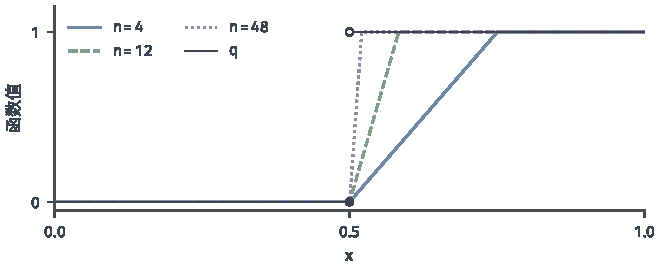
\includegraphics[width=112mm]{figures/00-shared/mathematical-preliminaries-upper/05-space-and-geometry/matplotlib/comprehension-additions/functional-incomplete-continuous.pdf}
  \caption{连续斜坡$u_n(t)=\operatorname{clip}(n(t-1/2),0,1)$取$n=4,12,48$（实、虚、点线），灰黑阶跃为$q=\mathbb I\{t>1/2\}$。黑实点与空心圈标明阶跃在$1/2$处的取值；斜坡逐点趋于阶跃，但$\|u_n-q\|_2^2=1/(3n)\to0$，$u_n$在一致范数下并不收敛到任何连续函数。图说明$C([0,1])$在$L^2$范数下不闭，不表示该阶跃有连续代表。}
  \label{fig:vol1-add-functional-incomplete-continuous}
\end{figure}

后面Riesz表示对闭零空间使用这条投影；正交系数对有限方向的张成使用这条投影。一般闭凸集合上的最近点涉及变分不等式，留给函数值拟合任务处理，因为那里改变的是可行集合，而非线性记录方向。

\subsubsection{有界线性泛函与Riesz表示}
\label{subsubsec:riesz-representation}

\paragraph{标量读取与有界性}

固定实Hilbert空间$H$，映射$L:H\to\mathbb R$称为\term{线性泛函}，若
\[
L(af+bg)=aL(f)+bL(g)\qquad(\forall f,g\in H,\ a,b\in\mathbb R).
\]
它把一个函数读成一个标量。若存在与$f$无关的常数$C$使
\[
|L(f)|\le C\|f\|\qquad(\forall f\in H),
\]
则称$L$有界，并定义最佳常数
\[
\|L\|=\sup_{\|f\|\le1}|L(f)|.
\]
有界性是“单位球上的输出有统一界”，与某个具体$f$的输出数值有限不是同一回事。

每个固定方向$h\in H$都给出一个有界读取$L_h(f)=\langle f,h\rangle_H$：由Cauchy–Schwarz，$|L_h(f)|\le\|h\|\|f\|$，故$\|L_h\|\le\|h\|$；取$f=h/\|h\|$（$h\ne0$）时$L_h(f)=\|h\|$，反向不等式成立，$\|L_h\|=\|h\|$。自然的反向问题是：每一个有界线性读取是否都来自某个固定方向？下面的Riesz表示给出肯定回答。

\paragraph{由零空间投影证明表示}

\begin{theorem}[Riesz表示]
\label{thm:riesz}
设$H$为实Hilbert空间，$L:H\to\mathbb R$为有界线性泛函。则存在唯一的$h_L\in H$，使
\begin{equation}
\label{eq:functional-riesz-representation}
L(f)=\langle f,h_L\rangle_H\qquad(\forall f\in H),
\end{equation}
且$\|L\|=\|h_L\|_H$。
\end{theorem}

\begin{proof}
若$L=0$，取$h_L=0$即可。下设$L\ne0$。

零空间$N=\{f\in H:L(f)=0\}$是$H$的线性子空间。它闭：若$f_n\in N$且$f_n\to f$，由有界性$|L(f)|=|L(f)-L(f_n)|\le\|L\|\|f-f_n\|\to0$，故$f\in N$。

取$v\in H$使$L(v)\ne0$。设$v=p+w$为$v$在$N$上的正交投影分解：$p=P_Nv\in N$，$w=v-p\perp N$。由$L(w)=L(v)-L(p)=L(v)\ne0$知$w\ne0$。

对任意$f\in H$，构造
\[
f-\frac{L(f)}{L(w)}\,w.
\]
它在$L$下的像为$L(f)-\frac{L(f)}{L(w)}L(w)=0$，故属于$N$；而$w\perp N$，与$w$取内积得零：
\[
\langle f,w\rangle-\frac{L(f)}{L(w)}\|w\|^2=0,
\qquad\text{即}\qquad
\langle f,w\rangle=\frac{L(f)}{L(w)}\|w\|^2.
\]
令
\begin{equation}
\label{eq:functional-riesz-direction}
h_L=\frac{L(w)}{\|w\|^2}\,w,
\end{equation}
则$L(f)=\langle f,w\rangle\,L(w)/\|w\|^2=\langle f,h_L\rangle$，表示成立。

唯一性：若$h,h'$都满足$L(f)=\langle f,h\rangle=\langle f,h'\rangle$，则$\langle f,h-h'\rangle=0$对一切$f$成立；取$f=h-h'$得$\|h-h'\|^2=0$。

范数等式：由$|L(f)|\le\|h_L\|\|f\|$得$\|L\|\le\|h_L\|$。反向，$L(h_L)=\langle h_L,h_L\rangle=\|h_L\|^2$，故$\|h_L\|=|L(h_L)|/\|h_L\|\le\|L\|$。两端相等。
\end{proof}

表示结论只适用于已经有界的标量泛函。它不能事先证明任意点读数有界——那要在点值一节单独检验；也不能把输出为整条边界函数的迹算子缩成单个内积方向，因为迹的输出不是标量。有界性、标量输出、Hilbert内积三者齐备，Riesz才给出一个方向。

\subsection{正交展开与系数记录}
\label{subsec:orthogonal-expansions-coefficients}

本小节固定表示方向，研究已知函数如何按正交方向分解、截断后丢失多少，以及不同有限记录之间如何转换。三个子题按同一记录任务的组成分工：建立方向记录、评估有限保留、转换记录坐标。

\subsubsection{正交系数与函数展开}
\label{subsubsec:orthogonal-records}

\paragraph{正交方向与完整记录}

设$H$为实Hilbert空间，序列$(e_j)_{j\ge1}\subset H$满足
\[
\langle e_j,e_k\rangle_H=\delta_{jk}.
\]
称$(e_j)$为正交归一序列；若所有有限线性组合在$H$中稠密，即$\overline{\operatorname{span}}\{e_j\}=H$，则称它为$H$的\term{完备正交系}（也叫正交归一基）。环境空间完备不等于所选正交系覆盖全部方向：在$\ell^2$中取仅偶数坐标非零的方向$e_2,e_4,\dots$，它们正交归一，其闭张成是$\ell^2$的真闭子空间，奇数方向整个缺失。

对前$m$个方向的张成$S_m=\operatorname{span}\{e_1,\dots,e_m\}$使用正交投影定理。$S_m$有限维因而闭。记$c_j=\langle f,e_j\rangle$，则
\begin{equation}
\label{eq:functional-orthogonal-partial-projection}
P_{S_m}f=\sum_{j=1}^m c_j e_j.
\end{equation}
验证：右端属于$S_m$，且对每个$k\le m$，$f-\sum_{j\le m}c_je_j$与$e_k$的内积为$c_k-c_k=0$，故与整个$S_m$正交。每个系数$c_j$正是前一小节$h_L=e_j$时的有界标量读取，$|c_j|\le\|f\|$。

正交性给出逐项相消的误差：
\begin{equation}
\label{eq:functional-bessel}
\|f-P_{S_m}f\|^2=\|f\|^2-\sum_{j=1}^m|c_j|^2,
\end{equation}
因而Bessel不等式$\sum_{j=1}^m|c_j|^2\le\|f\|^2$对一切$m$成立，正项级数$\sum_j|c_j|^2$收敛且不超过$\|f\|^2$。

\begin{theorem}[完备正交系与Parseval等式]
\label{thm:parseval}
设$(e_j)$为$H$的完备正交系，$c_j=\langle f,e_j\rangle$。则
\[
\begin{aligned}
\lim_{m\to\infty}\|f-\sum_{j=1}^m c_je_j\|=0,
\qquad
\|f\|^2=\sum_{j=1}^\infty|c_j|^2,\\
f=\sum_{j=1}^\infty c_je_j\quad(\text{依}H\text{范数}).
\end{aligned}
\]
\end{theorem}

\begin{proof}
记$s_m=\sum_{j\le m}c_je_j=P_{S_m}f$。由$S_m$张成在$H$中稠密，对$\varepsilon>0$存在有限组合$u=\sum_{j\le m_0}a_je_j$使$\|f-u\|<\varepsilon$。$s_{m_0}$是$f$在$S_{m_0}$上的最佳逼近，故$\|f-s_{m_0}\|\le\|f-u\|<\varepsilon$；而由Bessel误差公式，$\|f-s_m\|^2$随$m$增大单调不增（尾余项为正项级数尾和），故对一切$m\ge m_0$，$\|f-s_m\|<\varepsilon$。范数展开与Parseval等式随之成立。
\end{proof}

若正交系不完备，$P_{S_m}f$只收敛到$f$在其闭张成上的投影，正交余部$\overline{\operatorname{span}}\{e_j\}^\perp$中的分量永远保留。Bessel不等式与Parseval等式的差别正是覆盖条件的差别，不能混用。

\paragraph{傅里叶方向的计算与遗漏}

在$L^2([-\pi,\pi],\mathrm dx)$中取\term{傅里叶基}，即
\[
e_0=\frac1{\sqrt{2\pi}},\qquad
e_j^c=\frac{\cos(jx)}{\sqrt\pi},\qquad
e_j^s=\frac{\sin(jx)}{\sqrt\pi}\quad(j\ge1).
\]
直接积分给出
\[
\begin{aligned}
\int_{-\pi}^{\pi}\cos(jx)\cos(kx)\,\mathrm dx=\pi\delta_{jk},
\qquad
\int_{-\pi}^{\pi}\sin(jx)\sin(kx)\,\mathrm dx=\pi\delta_{jk},\\
\int_{-\pi}^{\pi}\cos(jx)\sin(kx)\,\mathrm dx=0.
\end{aligned}
\]
它们构成正交归一系；经典三角级数理论给出其完备性。正交评估的是函数内积：例如$1$与$x$的乘积在正负半区间相消，不等于“平面图像互相垂直”这种几何画面。

取$f(x)=x$。$f$是奇函数，故常数项与全部余弦系数为零。对第一个正弦方向分部积分：
\[
\begin{aligned}
\int_{-\pi}^{\pi}x\sin x\,\mathrm dx
&=\bigl[-x\cos x\bigr]_{-\pi}^{\pi}+\int_{-\pi}^{\pi}\cos x\,\mathrm dx\\
&=-\pi(-1)+\pi(-1)\cdot(-1)+0=2\pi,
\end{aligned}
\]
故第一个正弦系数为
\[
\frac1{\sqrt\pi}\int_{-\pi}^{\pi}x\sin x\,\mathrm dx=2\sqrt\pi.
\]
一般地，$\frac1{\sqrt\pi}\int_{-\pi}^{\pi}x\sin(jx)\,\mathrm dx=2\sqrt\pi\,(-1)^{j+1}/j$。Parseval等式此时成为可复算的检验：
\[
\sum_{j=1}^\infty\frac{4\pi}{j^2}=\frac{2\pi^3}{3}=\int_{-\pi}^{\pi}x^2\,\mathrm dx,
\]
其中$\sum_j1/j^2=\pi^2/6$。

保留常数及前$m$组正弦、余弦即得傅里叶截断。只取余弦方向时投影恒为零，增加再多同类方向也不能逼近$x$——方向选错时数量不补覆盖。完整三角系在上述$L^2$范数下完备，但范数收敛不自动承诺逐点收敛或一致收敛；截断误差在下一小节专门计算。

\subsubsection{正交截断与尾误差}
\label{subsubsec:truncation-tail}

固定同一$f$与同一完备正交系，只改变保留项数$m$，$s_m=\sum_{j\le m}c_je_j$是一个函数序列。由上节误差公式，
\begin{equation}
\label{eq:functional-truncation-tail}
\|f-s_m\|^2=\sum_{j>m}|c_j|^2\longrightarrow0,
\end{equation}
收敛来自可求和级数$\sum_j|c_j|^2$的尾部消失。每个$s_m$在当前前$m$个方向内最佳，但这并未与所有同规模非线性表示作比较——表示方向怎样选择由有限表示任务处理，这里固定方向后只回答截断是否收敛。

式\eqref{eq:functional-truncation-tail}只控制所选空间范数。点值误差要等点值读取建立相应有界常数后才能传递；一致误差还要求对所有位置有统一的读取界。不能从$L^2$尾项直接跳到逐点或一致收敛。另外，积分谱中的$L^2$归一方向与核RKHS中的归一方向尺度不同，相应的两种尾误差在Mercer展开处分别给出，此处不提前引入尚未定义的权重。

\subsubsection{系数与有限读数的转换}
\label{subsubsec:record-conversion}

\paragraph{换基与记录矩阵}

先限定$f=\sum_{j=1}^m a_j\varphi_j$属于已知有限维张成。线性无关的方向使系数由函数唯一确定；方向相关时，不同系数组可表示同一函数；一般非线性参数族则不能套用线性基的结论。

对$f(t)=a+bt$，把基$(1,t)$改为$(1,t-c)$，逐项展开
\[
f(t)=a+bt=(a+bc)+b(t-c),
\]
新系数为$(a+bc,b)$。这只改变记录坐标，目标函数及其取值完全相同。改读$f(0),f(1)$时，
\[
\begin{pmatrix}f(0)\\f(1)\end{pmatrix}
=\begin{pmatrix}1&0\\1&1\end{pmatrix}\begin{pmatrix}a\\b\end{pmatrix},
\]
由$f(0)=a$、$f(1)-f(0)=b$恢复系数。若只读$f(0)$，斜率方向不可见：可逆矩阵与缺失列分别意味着记录完整与方向丢失。

对一般线性读数$L_i$（$i=1,\dots,n$），记录矩阵$A\in\mathbb R^{n\times m}$的第$(i,j)$项为
\[
A_{ij}=L_i(\varphi_j).
\]
点值读数给出$A_{ij}=\varphi_j(x_i)$，积分读数给出$A_{ij}=\int\varphi_j w_i\,\mathrm d\mu$。代入前须核对定义域、积分存在与输出类型，再执行矩阵换算$L(f)=Aa$。

\paragraph{有限表示之外的边界}

矩阵可逆只说明：在指定的有限维候选张成内部，记录与系数的转换唯一。若候选扩大到任意函数，同样$n$条读数可能对应无穷多个函数——这是新增的单射性问题，交给有限读数的可识别性任务，不在已知表示的换算中提前宣告恢复成功。无限表示还须指定收敛范数、尾误差和极限归属；上面的正交截断提供了一种可核验情形，其他表示按各自条件判断，不能把有限求和矩阵原样当成无限展开的计算保证。

\subsection{点值与边界读取}
\label{subsubsec:point-boundary-readouts}

本小节按输出位置区分单点取值与整条边界记录。前者输出标量，后者通常输出边界函数等价类。共同要求是：先明确输入元素和合法代表，再判断读取是否存在并受范数控制。

\subsubsection{域内点值读取}
\label{subsubsec:point-evaluation}

\paragraph{等价类与合法代表}

在通常Lebesgue测度的$[0,1]$上，零函数与仅在$x=1/2$取$1$的函数是同一个$L^2$元素，却给出不同的点值。因此任取一个可测代表再读取该点，不能在商空间上定义同一个数：点值读取首先不是“是否有界”，而是“在等价类上是否良定义”。

该反例依赖单点的可测性与零测度。若$\mu(\{x\})>0$，两个几乎处处相等的代表在$x$处必相等，且有限$p$时
\[
|f(x)|\le\mu(\{x\})^{-1/p}\|f\|_p,
\]
正质量单点要另作判断，不能把零测点的结论推广到所有测度。

若某等价类存在连续代表，且测度在定义域上全支撑，则这样的代表唯一：两个连续代表若在一点不同，差异会延伸到一个正测度邻域，与几乎处处相等矛盾。这里解决的是唯一性；代表是否存在仍需额外正则性结论。若输入本来就是真实连续函数，或已由条件选出唯一连续代表，点读数有确定含义，但这个数是否被当前范数控制仍未解决。

\paragraph{点值的有界性与维数条件}

对已经良定义的线性点读数$L_x(f)=f(x)$，提出有界性要求
\[
|L_x(f)|\le C_x\|f\|,
\]
其中$C_x$可依赖位置$x$，但不能依赖$f$。在$[0,1]$上取连续尖峰
\[
f_n(t)=\max(1-nt,0),
\]
直接算得$\|f_n\|_2^2=\int_0^{1/n}(1-nt)^2\mathrm dt=1/(3n)$，而$f_n(0)=1$，比值$\sqrt{3n}$无界。故连续函数上的$L^2$范数不能控制原点读取；零点是闭区间中允许的输入位置，此例不替代一般区域的边界迹定理。

与积分读取对照：$L_w(f)=\int fw\,\mathrm d\mu$在$w\in L^2$时由Cauchy–Schwarz给出$|L_w(f)|\le\|w\|_2\|f\|_2$；正交系数也是这类内积读取。问题出在点读数与所选范数的组合，而非线性读取本身。

在一维有界区间$I=(a,b)$上，Sobolev范数确实控制点值，下面把这件事完整做完。设$u\in H^1(I)$，弱导$g\in L^2(I)$。令
\[
F(x)=\int_a^x g(t)\,\mathrm dt.
\]
积分基本定理给出$F$绝对连续；分部积分核对其弱导为$g$，故$u-F$的分布导数为零。要得到$u$的点值，还须说明零分布导数迫使$u-F$为常数。

设$T_{u-F}$为$u-F$诱导的分布。先取积分为零的紧支撑光滑测试$\psi$：其积分原函数$\varphi(x)=\int_a^x\psi$仍紧支撑且$\varphi'=\psi$，由$u-F$分布导数为零得
\[
0=\int(u-F)\varphi'=\int(u-F)\psi.
\]
固定一个积分为$1$的测试$\rho$。任意测试$\psi$可分解为$(\int\psi)\rho+\bigl(\psi-(\int\psi)\rho\bigr)$，第二项积分为零，被上式灭掉；于是
\[
T_{u-F}(\psi)=c\int\psi,\qquad c=T_{u-F}(\rho).
\]
即分布$T_{u-F}$等于常数$c$作为普通函数的分布。由普通函数表示分布的唯一性，$u-F=c$几乎处处。于是$c+F$是$u$的绝对连续代表，其每一点值合法且唯一。

记区间长度$L=b-a$。由平方积分平均，存在$y\in I$使
\[
|u(y)|\le L^{-1/2}\|u\|_2.
\]
对闭区间中任意$x$，$u(x)-u(y)=\int_y^x g$，再用Cauchy–Schwarz，
\begin{equation}
\label{eq:functional-point-evaluation-embed}
|u(x)|\le L^{-1/2}\|u\|_2+L^{1/2}\|g\|_2.
\end{equation}
该估计对闭区间中的$x$统一成立：一维$H^1$既解决单点有界，也给出全域控制。

一维结论不能跨维照搬。在三维域内部固定$x_0$，取光滑紧支撑$\varphi$且$\varphi(0)=1$，令$f_n(x)=\varphi(n(x-x_0))$，$n$足够大时支撑在域内。换元给出
\[
\|f_n\|_2^2=n^{-3}\|\varphi\|_2^2,\qquad
\|\nabla f_n\|_2^2=n^{-1}\|\nabla\varphi\|_2^2,\qquad
f_n(x_0)=1.
\]
于是$f_n(x_0)/\|f_n\|_{H^1}\asymp n^{1/2}\to\infty$：即使限制光滑函数，三维$H^1$范数也不能控制该点读数。一般逐点常数$C_x$可随位置增长，只有$\sup_xC_x<\infty$才给统一控制。取整条实轴上由$f(t)=bt$组成、范数为$|b|$的函数空间，点读数常数恰为$|x|$；真正把输入域限制为$[-3,3]$，才能取得统一常数$3$——图\ref{fig:vol1-add-functional-pointwise-bound-growth}同时画出两条单位范数函数与逐点常数，注意显示窗口不是定义域，$C_x$在实轴上无界。

\begin{figure}[h]
  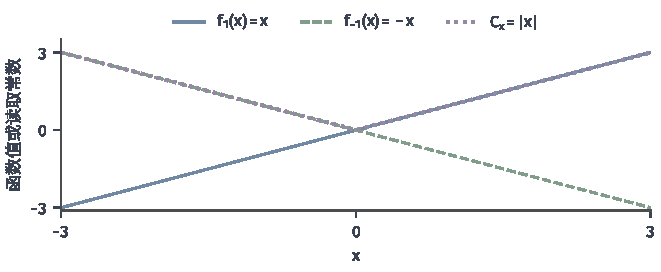
\includegraphics[width=112mm]{figures/00-shared/mathematical-preliminaries-upper/05-space-and-geometry/matplotlib/comprehension-additions/functional-pointwise-bound-growth.pdf}
  \caption{在$H=\{f(t)=bt\}$、$\|f\|_H=|b|$的空间中，单位范数函数$f_1(t)=t$与$f_{-1}(t)=-t$（实、虚线），点$x$处的最佳读取常数$C_x=|x|$（点线）。$x$离原点越远，同样范数函数在该点的值越大；在整条实轴上$C_x$无界，统一读取界不存在。显示窗口$[-3,3]$不是输入域。}
  \label{fig:vol1-add-functional-pointwise-bound-growth}
\end{figure}

\paragraph{再生核Hilbert空间与正向表示}

在真实函数组成的实Hilbert空间$H$中，把每个点读数$L_x:f\mapsto f(x)$都有界作为空间条件，称这样的空间为\term{再生核Hilbert空间}（RKHS）。先有点读数有界，才能调用Riesz表示取得唯一$K_x\in H$使
\begin{equation}
\label{eq:functional-reproducing-property}
f(x)=\langle f,K_x\rangle_H\qquad(\forall f\in H).
\end{equation}
定义$K(x,z)=K_z(x)=\langle K_z,K_x\rangle_H$，称它为$H$的\term{再生核}。由内积对称性，$K(x,z)=K(z,x)$；对任意有限点组与系数，
\[
0\le\Big\|\sum_i a_iK_{x_i}\Big\|_H^2
=\sum_{i,j}a_ia_jK(x_i,x_j),
\]
故核对称且Gram矩阵半正定；满足这条Gram半正定性的$K$称为\term{正定核}。$K:X\times X\to\mathbb R$是标量核。

由Riesz最佳常数，
\begin{equation}
\label{eq:functional-rkhs-pointwise-bound}
\|L_x\|=\|K_x\|_H=\sqrt{K(x,x)}.
\end{equation}
核对角上界$K(x,x)\le M^2$才使同一个$M$控制所有点：这解释了何种空间结构支持统一读取。

固定仿射核$K(x,z)=1+xz$，令
\[
H=\{f(t)=a+bt\},\qquad
\langle a+bt,a'+b't\rangle_H=aa'+bb'.
\]
取$K_x(t)=1+xt$，逐项核对：
\[
\langle a+bt,K_x\rangle_H=a\cdot1+b\cdot x=a+bx=f(x),
\]
$\|f\|_H^2=a^2+b^2$，$\|K_x\|_H^2=1+x^2$。抽象的再生关系在这里有完整坐标计算。

\paragraph{由半正定核反向构造空间}

正向构造从空间出发得到核；反过来，固定非空集合$X$与实对称半正定核$K$，也能唯一造出以$K$为再生核的RKHS。

先用有限核截面的形式线性组合建立双线性型
\[
\Big\langle\sum_i a_iK_{x_i},\sum_jb_jK_{z_j}\Big\rangle
=\sum_{i,j}a_ib_jK(x_i,z_j).
\]
Gram二次型半正定只给出半内积：存在非零组合长度为零。半内积的Cauchy–Schwarz$|\langle f,g\rangle|\le\|f\|\|g\|$表明，零长度方向在每点读数均为零，并有
\[
|f(x)|=|\langle f,K_x\rangle|\le\sqrt{K(x,x)}\,\|f\|.
\]
因此先商去零长度方向，读取在商空间上良定义，不能直接声称半内积空间已是Hilbert空间。

对该内积空间作完备化。逐点读取界使每条Cauchy列在每个$x$处取得确定极限（$|f_n(x)-f_m(x)|\le\sqrt{K(x,x)}\|f_n-f_m\|$），并使等价Cauchy列定义同一函数。若完成后的元素在所有点为零，它与每个$K_x$正交；核截面张成稠密，故该元素为零——完备化到函数空间的表示因此单射。核截面内积与再生关系在极限下保留，得到以$K$为再生核的RKHS。任何其他同核RKHS在核截面张成上内积相同，由稠密性唯一延拓，故空间由核唯一确定。半正定允许有限Gram矩阵奇异，不能把“正定核”的常用约定误读为所有Gram矩阵严格正定。

这条构造只需集合与半正定核，不需事先给测度。后面的积分谱还要另给测度及连续性、紧性条件；RKHS是具有稳定点读数的Hilbert函数空间，不是与Hilbert空间或Banach空间互斥的类别。

\paragraph{固定点的函数误差与位置误差}

先固定$x$和核空间，仅把$f$改为$f+h$。由再生关系，
\begin{equation}
\label{eq:functional-rkhs-error-fixedpoint}
|(f+h)(x)-f(x)|=|\langle h,K_x\rangle_H|
\le\sqrt{K(x,x)}\,\|h\|_H.
\end{equation}
这是有界读取在固定点的应用。再固定同一$f$，只把位置$x$改为$z$：
\[
f(x)-f(z)=\langle f,K_x-K_z\rangle_H,
\]
故
\[
\begin{aligned}
|f(x)-f(z)|\le\|f\|_H\|K_x-K_z\|_H,\\
\|K_x-K_z\|_H^2=K(x,x)+K(z,z)-2K(x,z).
\end{aligned}
\]
位置稳定取决于核截面在空间范数中的接近。若$X$有拓扑且$K$连续，上式给出核截面随位置连续，进而给出每个$f\in H$的连续性；若还要对一整类函数统一控制，则固定该类的范数半径。单点读取有界本身未包含位置连续性，两种扰动不能混成一项。

\subsubsection{边界迹与零边界空间}
\label{subsubsec:trace-zero-boundary}

弱导空间首先由体内几乎处处等价类组成；边界条件需要一条由体内元素到边界记录的合法映射，不能任取代表后逐点限制。

\paragraph{迹的输出与连续延拓}

固定有界Lipschitz区域$\Omega\subset\mathbb R^d$、边界表面测度$\mathrm dS$与输入空间$H^1(\Omega)$。所需输出是$L^2(\partial\Omega,\mathrm dS)$中的边界函数等价类，不是某个边界点上的标量，因而不是一个Riesz方向可以表示的对象。

在光滑函数上，限制$u\mapsto u|_{\partial\Omega}$就是熟悉的边界取值。把它延拓到整个$H^1(\Omega)$需要一个前提估计。标准迹定理指出：对上述Lipschitz区域，存在常数$C_\Omega$使
\begin{equation}
\label{eq:functional-trace-inequality}
\|u|_{\partial\Omega}\|_{L^2(\partial\Omega,\mathrm dS)}
\le C_\Omega\|u\|_{H^1(\Omega)}
\qquad(\forall u\in C^\infty(\overline\Omega)).
\end{equation}
其证明通过边界局部平直化，把问题化到半空间的一维论证（与本节端点估计同源），再用光滑逼近完成；一维区间上的端点估计式\eqref{eq:functional-point-evaluation-embed}是它最简单的特例，不能冒充一般区域的证明。

对任意$u\in H^1(\Omega)$，取光滑逼近列$u_n\in C^\infty(\overline\Omega)$在$H^1(\Omega)$中收敛于$u$。由式\eqref{eq:functional-trace-inequality}，
\[
\|u_n|_{\partial\Omega}-u_m|_{\partial\Omega}\|_{L^2(\partial\Omega)}
\le C_\Omega\|u_n-u_m\|_{H^1(\Omega)},
\]
故边界限制列在$L^2(\partial\Omega)$中为Cauchy列。$L^2$完备，取得极限；若另取逼近列$v_n\to u$，混合列$(u_1,v_1,u_2,v_2,\dots)$同样$H^1$收敛，其边界列极限唯一，故极限与逼近列选择无关。以此定义连续延拓
\[
\operatorname{Tr}:H^1(\Omega)\to L^2(\partial\Omega,\mathrm dS),
\]
并保留同一范数界$\|\operatorname{Tr}u\|_{L^2(\partial\Omega)}\le C_\Omega\|u\|_{H^1(\Omega)}$。迹算子是有界线性算子，其输出类型为边界函数等价类。

\paragraph{零迹与固定边界的可行集合}

用$H^1$范数闭包定义
\[
H_0^1(\Omega)=\overline{C_c^\infty(\Omega)}^{\,H^1(\Omega)},
\]
该定义不依赖任意代表的逐点边界值。由$\operatorname{Tr}$连续且$C_c^\infty(\Omega)$中函数在边界附近为零，$H_0^1\subseteq\ker\operatorname{Tr}$。标准零迹刻画定理给出反向包含：在上述Lipschitz区域条件下，$\ker\operatorname{Tr}$恰为$C_c^\infty(\Omega)$的$H^1$闭包，故
\[
H_0^1(\Omega)=\ker\operatorname{Tr}.
\]

迹的像不能直接当成全部$L^2$边界函数。若已知合法边界数据$g=\operatorname{Tr}G$，候选集合可写成$G+H_0^1(\Omega)$：允许扰动具有零迹。这为后面的梯度拟合提供不依赖点值代表的边界接口。自由边界则允许相应边界扰动；具体自然通量由变分任务及额外正则性推导，此处不提前给所有弱解定义普通法向导数。

\section{线性算子与积分方程}
\label{sec:linear-operators-integral-equations}

本节研究函数空间之间的线性运算及其方程：先建立各类运算共用的定义域、范数与算子性质，再对积分算子检查作用是否合法、怎样改变方向，最后求解该积分运算进入的方程。共用准备与两个主体任务分别标明，不能把一般算子性质藏在积分核的例子里，也不能把求解方程与已知函数的正向积分混成同一种输出。

\subsection{线性算子的共同框架}
\label{subsec:operator-framework}

本小节只建立后面确实使用的输入输出、误差范数、伴随与紧性语言。点读数和投影是已经见过的实例，微分与迹说明定义域和目标空间也可能改变。

\subsubsection{定义域、有界性与输入误差}
\label{subsubsec:operator-domain-boundedness}

\paragraph{线性算子及所用范数}

固定赋范空间$V,W$，映射$A:V\to W$称为线性算子，若
\[
A(af+bg)=aAf+bAg.
\]
若实际只允许定义域$D(A)\subset V$中的输入，应在一开始写清该线性定义域；函数、导数或积分存在的成员条件不能省略成一个形式公式。有界算子框架先取$A$在整个$V$上定义；若只取受限定义域，须另写其所赋范数，不自动调用全空间结论。

定义算子范数
\[
\|A\|_{\mathrm{op}}=\sup_{\|f\|_V\le1}\|Af\|_W.
\]
其有限等价于存在统一常数$C$使$\|Af\|_W\le C\|f\|_V$，最佳常数就是$\|A\|_{\mathrm{op}}$。这里的有界是单位球输出有统一界，与某个输入的输出数值有限不同；对线性算子，这一条件也等价于连续性。

用同一求导公式比较定义域和范数：$D:H^1(I)\to L^2(I)$在Sobolev范数下有界，因为$\|u'\|_2\le\|u\|_{H^1}$。仅用$L^2$输入范数时，在$I=(0,2\pi)$取$f_n(x)=\sin(nx)$，则
\[
\|f_n\|_2=\sqrt\pi,\qquad \|f_n'\|_2=n\sqrt\pi,
\]
比值$n$无界，不存在统一的导数控制常数。因此不能不核对空间，就给微分运算套用后面有界紧算子的结论。

\paragraph{固定算子的输入误差传播}

固定$A$及两空间范数，输入由$f$变为$f+h$。线性先把输出差化为$Ah$，再由算子范数，
\begin{equation}
\label{eq:functional-operator-error-propagation}
\|A(f+h)-Af\|_W=\|Ah\|_W\le\|A\|_{\mathrm{op}}\|h\|_V.
\end{equation}
没有线性时，不能从“输出有界”直接写出这一差分界。正交系数、固定点值、边界迹和后面的积分算子分别在自己的输入输出范数下代入常数；位置变化由核截面差处理，数据变化后重新优化则是解映射稳定性，二者均不是这条固定算子界自动包办的结论。

\subsubsection{伴随、自伴、正与紧}
\label{subsubsec:adjoint-selfadjoint-compact}

\paragraph{伴随与二次型}

在实Hilbert空间$V,W$中固定有界线性$A:V\to W$。对每个$w\in W$，映射$f\mapsto\langle Af,w\rangle_W$是$V$上的有界标量泛函：
\[
|\langle Af,w\rangle_W|\le\|Af\|_W\|w\|_W\le\|A\|_{\mathrm{op}}\|f\|_V\|w\|_W.
\]
由Riesz表示，存在唯一$A^*w\in V$使
\[
\langle Af,w\rangle_W=\langle f,A^*w\rangle_V.
\]
$A^*$的线性：对$w_1,w_2$，$\langle f,A^*(w_1+w_2)\rangle=\langle Af,w_1+w_2\rangle=\langle f,A^*w_1+A^*w_2\rangle$对一切$f$成立，故$A^*(w_1+w_2)=A^*w_1+A^*w_2$；齐次性同理。由$|\langle Af,w\rangle|\le\|A\|\|f\|\|w\|$取得$\|A^*w\|\le\|A\|\|w\|$，故$A^*$有界且$\|A^*\|\le\|A\|$。反过来，
\[
\|Af\|_W=\sup_{\|w\|\le1}|\langle Af,w\rangle_W|
=\sup_{\|w\|\le1}|\langle f,A^*w\rangle_V|
\le\|A^*\|\|f\|_V,
\]
故$\|A\|\le\|A^*\|$，两端相等$\|A^*\|=\|A\|$。

仅当输入输出为同一Hilbert空间时定义自伴$A=A^*$。本节的正算子约定为自伴且$\langle Af,f\rangle\ge0$：自伴允许负二次型，正性另加非负要求，二者不能只凭核对称一并得到。

\paragraph{紧性及其与有界性的区别}

线性算子$A:V\to W$称为紧算子，若它把$V$中有界集合映为$W$中相对紧集合；等价地，每个有界输入列$(f_n)$的输出列$(Af_n)$有范数收敛子列。有限秩有界算子的输出落在有限维空间的有界集中，故紧。

在无限维Hilbert空间用正交归一序列检验恒等算子$I$：各$\|e_n\|=1$，$\|e_n-e_m\|=\sqrt2\ (n\ne m)$，输出列没有收敛子列，故$I$不紧。$I$有界、自伴且正，却不紧——前三种条件不替代紧性。

紧算子的算子范数极限仍紧，这是后面核逼近的桥梁。设$A_n\to A$（$\|A_n-A\|\to0$），$A_n$紧。对单位球输出$A(B)$：取$n$使$\|A_n-A\|<\varepsilon$，$A_n(B)$相对紧故有有限$\varepsilon$-网$\{y_i\}$。任取$Af$，选$y_i$使$\|A_nf-y_i\|<\varepsilon$，则
\[
\|Af-y_i\|\le\|(A-A_n)f\|+\|A_nf-y_i\|<\varepsilon+\varepsilon=2\varepsilon,
\]
故$\{y_i\}$是$A(B)$的$2\varepsilon$-网。$W$完备使闭包紧，故$A(B)$相对紧。

\subsubsection{群平均与不变方向}
\label{subsubsec:group-average}

这项沿用已建立的投影和有界算子语言，给出已知函数运算如何主动消去方向的实例。

\paragraph{群平均与不可见方向}

固定有限群$G$在函数定义域上的作用，定义
\[
Pf(x)=\frac1{|G|}\sum_{g\in G}f(gx).
\]
若放在$L^2(\mu)$中，还要求作用可测且保测度，使输入等价类上的复合与范数控制合法。群乘法是双射重排求和，故
\[
P f(hx)=\frac1{|G|}\sum_g f(ghx)=\frac1{|G|}\sum_{g'}f(g'x)=Pf(x),
\]
输出不变。重复平均给出$P^2=P$。再证自伴：对任意$h\in L^2(\mu)$，作变量替换$y=gx$并用保测度与取逆重排，
\[
\begin{aligned}
\langle Pf,h\rangle
&=\frac1{|G|}\sum_{g\in G}\int f(gx)h(x)\,\mathrm d\mu(x)\\
&=\frac1{|G|}\sum_{g\in G}\int f(y)h(g^{-1}y)\,\mathrm d\mu(y)\\
&=\int f(y)\Bigl(\frac1{|G|}\sum_{g'\in G}h(g'y)\Bigr)\,\mathrm d\mu(y)\\
&=\langle f,Ph\rangle.
\end{aligned}
\]
$P$幂等且自伴，故它是到不变函数闭子空间的正交投影。

在对称区间及对称测度上取$G=\{I,-I\}$，得$Pf(x)=[f(x)+f(-x)]/2$：偶方向保留、奇方向消去，特别是$f(x)=x$输出零。同样在中心对称的二维区域上，横坐标$f(x_1,x_2)=x_1$也被平均为零。被主动移除的信息可能正是任务需要的方向，故这种不变性不单独给出预测或泛化保证。

\subsection{积分算子的作用与方向}
\label{subsubsec:integral-operator-directions}

固定标量核和测度后，积分算子把已知函数送成另一个函数（积分结果函数）。点值核表示可在附加条件下提供同一核，但一般可积核允许正负：它既不必正定，也不是输出非负测度的测度核。

\subsubsection{平方可积核的有界性与紧性}
\label{subsubsec:hilbert-schmidt}

\paragraph{从核截面取得整函数输出}

这里讨论的是由各位置的积分值组成的整个输出函数，不涉及复分析中的整函数概念。
固定$\sigma$有限测度空间$(X,\mu)$、$(Y,\nu)$以及
\[
K\in L^2(Y\times X,\nu\otimes\mu).
\]
对$f\in L^2(X,\mu)$写
\begin{equation}
\label{eq:functional-kernel-integral-operator}
(T_Kf)(y)=\int_X K(y,x)f(x)\,\mathrm d\mu(x).
\end{equation}
先说明这次作用合法。由Fubini定理，对$\nu$几乎处处的$y$，核截面$K(y,\cdot)\in L^2(X,\mu)$；由Cauchy–Schwarz，
\[
|(T_Kf)(y)|\le\|K(y,\cdot)\|_{L^2(\mu)}\|f\|_{L^2(\mu)},
\]
故积分对这样的$y$存在有限，输出按$\nu$几乎处处等价类理解。对$y$积分：
\begin{equation}
\label{eq:functional-hilbert-schmidt-bound}
\|T_Kf\|_{L^2(\nu)}
\le\left(\int_Y\|K(y,\cdot)\|_{L^2(\mu)}^2\,\mathrm d\nu(y)\right)^{1/2}\|f\|_{L^2(\mu)}
=\|K\|_{L^2(\nu\otimes\mu)}\|f\|_{L^2(\mu)}.
\end{equation}
$T_K:L^2(\mu)\to L^2(\nu)$有界；平方可积核产生的这类运算称为Hilbert–Schmidt积分算子。前述输入误差传播界可使用这里的上界；测度及其归一化都是算子定义的一部分。

\paragraph{由有限秩逼近得到紧性}

有限矩形指示函数的线性组合在乘积$L^2(\nu\otimes\mu)$中稠密（$\sigma$有限性支持先在有限测度块上完成逼近），故可取$K_n\to K$于$L^2(Y\times X)$。每个矩形核$K_n(y,x)=\sum_{i=1}^r\varphi_i(y)\psi_i(x)$把$f$送成
\[
T_{K_n}f=\sum_{i=1}^r\Big(\int_X\psi_i f\,\mathrm d\mu\Big)\varphi_i,
\]
输出落在固定的有限维$\operatorname{span}\{\varphi_i\}$中，故对应有限秩有界算子。对核差重复式\eqref{eq:functional-hilbert-schmidt-bound}的估计：
\[
\|T_{K_n}-T_K\|_{\mathrm{op}}\le\|K_n-K\|_{L^2(\nu\otimes\mu)}\to0.
\]
紧算子的算子范数极限仍紧，故$T_K$紧。由核平方可积到紧性的中间依据是有限秩逼近，不能从有界性直接跳到紧性。

若输入输出是同一测度空间，实核几乎处处对称（$K(y,x)=K(x,y)$ a.e.）使$T_K$自伴，因为
\[
\langle T_Kf,g\rangle=\iint K(y,x)f(x)g(y)\,\mathrm d\mu(x)\mathrm d\mu(y)
\]
关于$f,g$对称；正性仍须另查$\langle T_Kf,f\rangle\ge0$。对一般$L^2$核，任意点的核值甚至不由等价类决定，不能把算子二次型非负与逐点Gram矩阵半正定直接当成同一条件。

\subsubsection{紧自伴谱、零空间与Mercer展开}
\label{subsubsec:compact-spectrum-mercer}

\paragraph{积分作用保留和消去的方向}

先给出紧自伴算子的谱结构。设$T$为实Hilbert空间$H$上的紧自伴算子。

\begin{theorem}[紧自伴算子谱定理]
\label{thm:compact-selfadjoint}
设$T$为实Hilbert空间$H$上的紧自伴算子。则：
\begin{enumerate}
\item 非零特征值$\mu_j$为实数，两两正交归一的特征方向$\psi_j$可取为$H$中的正交归一系；每个非零特征空间有限维；
\item 非零特征值至多可数，按$|\mu_1|\ge|\mu_2|\ge\cdots$排列，唯一可能的聚点为$0$；
\item 非零特征方向的闭张成等于$(\ker T)^\perp$，故
\[
\begin{aligned}
H=\ker T\oplus\overline{\operatorname{span}}\{\psi_j\},\\
f=f_0+\sum_j b_j\psi_j,\quad b_j=\langle f,\psi_j\rangle,\quad f_0\in\ker T,
\end{aligned}
\]
且$Tf=\sum_j\mu_jb_j\psi_j$。
\end{enumerate}
\end{theorem}

\begin{proof}
第一步，证明$\|T\|_{\mathrm{op}}=\sup_{\|f\|=1}|\langle Tf,f\rangle|$。上界由Cauchy–Schwarz直接得到。反向：记$M=\sup_{\|f\|=1}|\langle Tf,f\rangle|$。由自伴，
\[
4\langle Tx,y\rangle=\langle T(x+y),x+y\rangle-\langle T(x-y),x-y\rangle,
\]
故
\[
|\langle Tx,y\rangle|\le\frac M4\bigl(\|x+y\|^2+\|x-y\|^2\bigr)
=\frac M2(\|x\|^2+\|y\|^2).
\]
对单位$x$取$y=Tx/\|Tx\|$，得$\|Tx\|\le M$，即$\|T\|_{\mathrm{op}}\le M$。

第二步，若$\|T\|_{\mathrm{op}}>0$，取单位列$f_n$使$|\langle Tf_n,f_n\rangle|\to\|T\|_{\mathrm{op}}$。该列的符号未必一致，故再抽子列（仍记为$f_n$）使$\langle Tf_n,f_n\rangle$的符号稳定为某个$\varepsilon\in\{+1,-1\}$；沿此子列记$\lambda=\varepsilon\|T\|_{\mathrm{op}}$，则$\langle Tf_n,f_n\rangle\to\lambda$（$T=0$时结论显然）。于是
\[
\begin{aligned}
\|Tf_n-\lambda f_n\|^2
&=\|Tf_n\|^2-2\lambda\langle Tf_n,f_n\rangle+\lambda^2\\
&\le\|T\|^2-2\lambda\langle Tf_n,f_n\rangle+\lambda^2\longrightarrow0.
\end{aligned}
\]
$T$紧，$(Tf_n)$有收敛子列；由$f_n=(Tf_n-(Tf_n-\lambda f_n))/\lambda$，$(f_n)$随之收敛到单位向量$f_*$，连续性给出$Tf_*=\lambda f_*$。$\lambda\ne0$为特征值。

第三步，非零特征空间有限维：若$\ker(T-\mu I)$（$\mu\ne0$）无限维，可取其中正交归一序列$(\varphi_n)$，则$\|T\varphi_n-T\varphi_m\|=|\mu|\|\varphi_n-\varphi_m\|=|\mu|\sqrt2$无收敛子列，与紧性矛盾。

第四步，不同特征值的特征方向正交：$T\psi=\mu\psi$，$T\varphi=\nu\varphi$，$\mu\ne\nu$，则
\[
\mu\langle\psi,\varphi\rangle=\langle T\psi,\varphi\rangle=\langle\psi,T\varphi\rangle=\nu\langle\psi,\varphi\rangle,
\]
故$\langle\psi,\varphi\rangle=0$。

第五步，归纳分裂。$T$在$E_\lambda=\ker(T-\lambda I)$的正交补上仍紧自伴；重复上述取得下一个模最大非零特征值，取得一列$|\mu_1|\ge|\mu_2|\ge\cdots$。对任意$\delta>0$，集合$\{|\mu|\ge\delta\}$中至多有有限个特征值：否则可取该集合中两两正交归一的特征方向列$\psi_j$，$T\psi_j=\mu_j\psi_j$，则$\|T\psi_j-T\psi_k\|\ge\delta$无收敛子列，与紧性矛盾。于是非零特征值至多可数（每个环带$\{1/(n+1)<|\mu|\le1/n\}$中有限个），且唯一可能的聚点为$0$。

第六步，闭张成与零空间互补。设$M=\overline{\operatorname{span}}\{\psi_j\}$。$M^\perp$上$T$的限制仍紧自伴且没有非零特征值；第二步的极值论证说明，任何非零紧自伴算子必有非零特征值，故该限制恒为零，即$M^\perp\subseteq\ker T$。反之，若$f\in\ker T$，
\[
\langle f,\psi_j\rangle=\frac1{\mu_j}\langle f,T\psi_j\rangle=\frac1{\mu_j}\langle Tf,\psi_j\rangle=0,
\]
故$\ker T\subseteq M^\perp$。两端相等，展开式成立。
\end{proof}

于是积分作用把非零方向各自按$\mu_j$缩放，把零空间完全消去。展开首先在$H$范数意义下成立，不等于核的逐点级数。

\paragraph{Mercer条件与两种空间尺度}

从一般紧自伴谱走向核的逐点表示，需要附加条件。标准Mercer定理指出：固定紧度量集合$X$、连续实对称半正定核$K$，以及$X$上有限正、全支撑Borel测度$\mu$，则$T_K$为$L^2(X,\mu)$上的紧自伴正算子（正特征值之和有限，即\term{迹类算子}），其非零特征值$\mu_j>0$对应可取连续代表的$L^2$归一特征函数$\psi_j$，且核本身有一致绝对收敛的展开
\begin{equation}
\label{eq:functional-mercer-expansion}
K(x,z)=\sum_{j=1}^\infty\mu_j\psi_j(x)\psi_j(z).
\end{equation}
核的连续性把$L^2$等价类意义下的特征函数提升为可作点值的连续代表；一般紧自伴结论没有这些逐点保证。零特征值方向不参与以上展开，不能对$\mu_j=0$使用除以$\mu_j$的公式。

与前面的RKHS构造衔接：$H_K$中函数由核连续性而连续，全支撑测度又保证它们作为$L^2$等价类的表示单射。在这些条件下，$\sqrt{\mu_j}\psi_j$构成$H_K$中的完备正交系（再生关系给出$\langle\psi_j,\psi_k\rangle_{H_K}=\delta_{jk}/\mu_j$），故$f=\sum_jb_j\psi_j$的连续代表属于$H_K$，当且仅当没有零谱分量且
\[
\sum_j\frac{b_j^2}{\mu_j}<\infty,
\]
且其核范数平方恰为该和。$L^2$归一坐标与$H_K$归一坐标相差$\sqrt{\mu_j}$因子：后续拟合与尾误差的权重由此而来。

\paragraph{正谱截断的两种尾误差}

对正谱闭张成中的$f=\sum_jb_j\psi_j$，固定截断$f_m=\sum_{j\le m}b_j\psi_j$。由$L^2$正交性，
\[
\|f-f_m\|_{L^2(\mu)}^2=\sum_{j>m}b_j^2.
\]
只要$f\in L^2$，该尾和随$m\to\infty$趋零；若原目标另有零谱分量$f_0$，误差还须保留$\|f_0\|_2^2$，不能声称截断趋向完整目标。

若进一步$f\in H_K$，改用核空间正交系得
\[
\|f-f_m\|_{H_K}^2=\sum_{j>m}\frac{b_j^2}{\mu_j}.
\]
若加权级数发散，核范数结论不适用；小$L^2$尾项不能替代小核范数尾项。对核范数收敛的截断，用固定点误差界取得每点控制
\[
|f(x)-f_m(x)|\le\sqrt{K(x,x)}\,\|f-f_m\|_{H_K};
\]
紧集上连续核的对角线$K(x,x)$有统一上界，因而还取得一致收敛。这是额外读取条件给出的结果，不是任意$L^2$正交展开自带的结论。

\paragraph{仿射核的完整谱计算}

固定$X=[-1,1]$、$K(x,z)=1+xz$与$\mathrm d\mu(z)=\mathrm dz/2$。直接积分
\[
(T_Kf)(x)=\int_{-1}^1(1+xz)f(z)\frac{\mathrm dz}{2}
=\int f\,\mathrm d\mu+x\int zf(z)\,\mathrm d\mu(z).
\]
对$f(z)=1+z$，$\int f\,\mathrm d\mu=1$、$\int zf(z)\,\mathrm d\mu=1/3$，输出为$1+x/3$（图\ref{fig:vol1-add-functional-integral-operator-action}）；若把测度改成$\mathrm dz$，两个积分加倍，输出变为$2+2x/3$——核公式相同不保证积分算子相同。

\begin{figure}[h]
  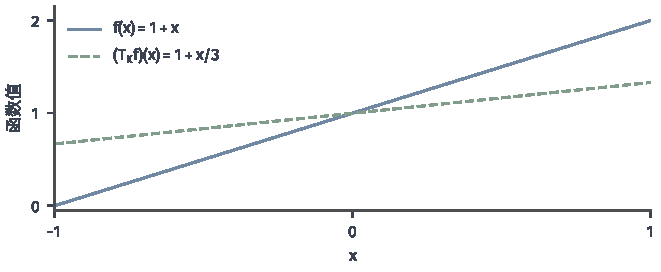
\includegraphics[width=112mm]{figures/00-shared/mathematical-preliminaries-upper/05-space-and-geometry/matplotlib/comprehension-additions/functional-integral-operator-action.pdf}
  \caption{$K(x,z)=1+xz$、$\mathrm d\mu=\mathrm dz/2$下，$f(x)=1+x$（实线）与其积分像$(T_Kf)(x)=1+x/3$（虚线）。积分把斜率压到原来的$1/3$，常数分量不动：正特征值$1$与$1/3$分别作用在常数与线性方向上。}
  \label{fig:vol1-add-functional-integral-operator-action}
\end{figure}

在归一测度下算谱。$T_K1=\int1\,\mathrm d\mu=1$，故$\psi_1=1$、$\mu_1=1$；$T_Kx=\int z\,\mathrm d\mu+x\int z^2\,\mathrm d\mu=x/3$，故$\psi_2=\sqrt3\,x$（归一：$\int 3x^2\,\mathrm d\mu=1$）、$\mu_2=1/3$。其余与$1,x$正交的方向属于零空间；两个正谱方向只覆盖仿射子空间，不能说整个$L^2[-1,1]$只有两个方向。

对$f=a+bx$，谱系数$b_1=\langle f,\psi_1\rangle=a$、$b_2=\langle f,\psi_2\rangle=b/\sqrt3$，故
\begin{equation}
\label{eq:functional-affine-two-norms}
\|f\|_{L^2(\mu)}^2=a^2+\frac{b^2}{3},\qquad
\|f\|_{H_K}^2=\frac{b_1^2}{\mu_1}+\frac{b_2^2}{\mu_2}=a^2+b^2.
\end{equation}
取$f=1+x$时两者分别为$4/3$和$2$；截到常数方向的尾误差平方分别为$1/3$和$1$，可与上面两种尾误差逐项核对。该谱例沿用前面同一仿射核空间，但额外加入测度后才取得积分特征值；改变测度会改变积分谱与$L^2$归一方向，不会自动改变原核通过再生关系定义的内积。

\subsection{积分方程的迭代求解}
\label{subsec:integral-equation-iteration}

前面给定函数计算积分输出；这里改为给定积分规则和外部项，寻找满足方程的未知函数。两项围绕同一名义方程，仅改变更新是否精确执行；表示截断与惩罚参数极限归入各自任务，不在这里混用。

\subsubsection{自映射与压缩条件}
\label{subsubsec:self-map-contraction}

固定$g\in C([a,b])$、紧矩形$[a,b]\times[a,b]$上连续的实核$K$与参数$\lambda$，要求未知函数$f\in C([a,b])$满足第二类Fredholm积分方程
\begin{equation}
\label{eq:functional-fredholm-equation}
f(x)=g(x)+\lambda\int_a^b K(x,t)f(t)\,\mathrm dt.
\end{equation}
把右端记为$Tf$：积分部分是线性算子，加入固定$g$后$T$是仿射映射。目标是求解该方程，即找$T$的不动点，而不只是生成一条没有解释对象的函数序列。

先核对$T$确实把$C([a,b])$映回自身。$K$在紧矩形上联合连续，故有界且一致连续。对固定连续$f$，
\[
|Tf(x)-Tf(z)|\le|g(x)-g(z)|+|\lambda|\|f\|_\infty\int_a^b|K(x,t)-K(z,t)|\,\mathrm dt;
\]
右端两项随$|x-z|\to0$一致趋于零，故$Tf$连续。$C([a,b])$在一致范数$\|\cdot\|_\infty$下完备。

接下来需要一个不动点存在定理，即\term{压缩映射}定理。它在本章本地完整建立，而不是引用别处结论。

\begin{theorem}[压缩映射定理（Banach不动点）]
\label{thm:banach-fixed-point}
设$(X,d)$为完备度量空间，$T:X\to X$满足压缩条件：存在$0\le q<1$使
\[
d(Tu,Tv)\le q\,d(u,v)\qquad(\forall u,v\in X).
\]
则$T$存在唯一不动点$x_*$。任取初值$x_0$，迭代$x_{k+1}=Tx_k$收敛于$x_*$，且
\begin{equation}
\label{eq:functional-iteration-apriori}
d(x_k,x_*)\le\frac{q^k}{1-q}\,d(x_1,x_0),
\end{equation}
\begin{equation}
\label{eq:functional-iteration-aposteriori}
d(x_k,x_*)\le\frac{q}{1-q}\,d(x_k,x_{k-1})\qquad(k\ge1).
\end{equation}
\end{theorem}

\begin{proof}
压缩映射连续：$d(Tx,Ty)\le q\,d(x,y)\to0$。逐步递推给出相邻步误差
\[
d(x_{n+1},x_n)\le q\,d(x_n,x_{n-1})\le\cdots\le q^n d(x_1,x_0).
\]
对$m>n$用三角不等式与几何级数，
\[
d(x_m,x_n)\le\sum_{j=n}^{m-1}d(x_{j+1},x_j)
\le d(x_1,x_0)\sum_{j=n}^{m-1}q^j
\le\frac{q^n}{1-q}d(x_1,x_0)\to0.
\]
$(x_n)$是Cauchy列；$X$完备，$x_n\to x_*$。由$T$连续，$Tx_*=\lim Tx_n=\lim x_{n+1}=x_*$，不动点存在。

唯一性：若$x_*,y_*$均为不动点，$d(x_*,y_*)=d(Tx_*,Ty_*)\le q\,d(x_*,y_*)$，$q<1$迫使$d(x_*,y_*)=0$。

先验界：在上面的逐步递推中令$m\to\infty$，
\[
d(x_*,x_n)\le\frac{q^n}{1-q}d(x_1,x_0).
\]
后验界：$d(x_n,x_*)\le q\,d(x_{n-1},x_*)$，故
\[
d(x_{n-1},x_*)\le d(x_{n-1},x_n)+d(x_n,x_*)\le d(x_{n-1},x_n)+q\,d(x_{n-1},x_*),
\]
整理得$(1-q)d(x_{n-1},x_*)\le d(x_{n-1},x_n)$，即$d(x_n,x_*)\le\frac{q}{1-q}d(x_n,x_{n-1})$。
\end{proof}

回到积分方程。对任意$f,h\in C([a,b])$，先在积分内作差再取绝对值，
\[
|Tf(x)-Th(x)|\le|\lambda|\|f-h\|_\infty\int_a^b|K(x,t)|\,\mathrm dt,
\]
故
\[
\|Tf-Th\|_\infty\le q\|f-h\|_\infty,\qquad
q=|\lambda|\sup_{x\in[a,b]}\int_a^b|K(x,t)|\,\mathrm dt.
\]
$q$必须对所有输入函数统一且满足$q<1$，不能用某次更新恰好变小代替严格压缩条件。自映射、完备与统一$q<1$齐备，定理\ref{thm:banach-fixed-point}给出唯一不动点$f_*$；由$T$的定义式，$f_*$正是方程\eqref{eq:functional-fredholm-equation}的解。

\subsubsection{精确更新与执行误差}
\label{subsubsec:exact-inexact-updates}

\paragraph{精确迭代的收敛与停止误差}

固定同一$g,K,\lambda$及初值$f^{(0)}\in C([a,b])$，令$f^{(k+1)}=Tf^{(k)}$。由刚核对的条件，精确迭代在一致范数中趋向唯一解$f_*$；方程与名义更新映射不变，变化的只是迭代中的近似函数。

先验界\eqref{eq:functional-iteration-apriori}说明误差只需初始更新差$\|f^{(1)}-f^{(0)}\|_\infty$与预先取得的$q$估计；后验界\eqref{eq:functional-iteration-aposteriori}说明已算出的相邻差$\|f^{(k)}-f^{(k-1)}\|_\infty$可直接用于停止判断。$q$接近一时必须保留$1/(1-q)$的放大因子：相邻变化小不直接等于误差同样小。$q\ge1$只使压缩论证失去保证，并不推出积分方程无解或多解；若要继续，须用别的条件另证。

\paragraph{同一方程下的扰动迭代}

保持同一名义$T$，实际更新未必精确执行：设
\[
\|f^{(k+1)}-Tf^{(k)}\|_\infty\le\eta_k,
\]
记$e_k=\|f^{(k)}-f_*\|_\infty$。先以三角不等式分离执行误差与名义输出差，再用压缩条件，
\begin{equation}
\label{eq:functional-perturbed-iteration}
e_{k+1}
\le\|f^{(k+1)}-Tf^{(k)}\|_\infty+\|Tf^{(k)}-Tf_*\|_\infty
\le\eta_k+q\,e_k.
\end{equation}
$\eta_k$可表示数值积分与更新造成的、对更新后整个函数的一致偏差，但不能把未经比较的模型差异也塞入其中。

反复展开递推：
\begin{equation}
\label{eq:functional-perturbed-unrolling}
e_k\le q^k e_0+\sum_{j=0}^{k-1}q^{\,k-1-j}\eta_j.
\end{equation}
初值影响随迭代按$q^k$衰减；历次执行误差按剩余更新次数加权。若$\eta_j\le\eta$一致，几何级数给出
\[
\limsup_{k\to\infty}e_k\le\frac{\eta}{1-q}.
\]
这是持续执行误差造成的误差地板上界，不保证每条轨迹收敛，更不保证误差恰好达到该边界。

若$\eta_j\to0$，把误差和分为有限早期项与尾部：对固定$J$，$j\le J$的有限项因几何权重$q^{k-1-j}\to0$而消失；$j>J$的尾部由$\sup_{j>J}\eta_j$乘$1/(1-q)$控制。取$J$足够大使尾部界任意小，再令$k\to\infty$，即得$e_k\to0$。更一般的可求和条件可作为同一分解的充分情形。比较持续与衰减执行误差时始终固定方程、初值和名义$q$，改变的仅是执行精度。若实际近似函数不在所定连续空间中，或自映射、完备、严格压缩任一项缺失，都须重建适用框架；这些限制与$q\ge1$的边界共同保留。
\section{泛函变分与函数拟合}
\label{sec:variational-functional-fitting}

前面各节把函数作为已知对象，研究怎样合法地读取它、用它构造算子或把它分解成正交方向。本节把函数改为未知量：候选函数本身是优化变量，我们要在给定候选空间、给定观测数据和给定偏差计量下，判断最优函数是否存在、是什么形状、对数据扰动有多敏感。三个任务分别规定不同的观测类型：有限个线性读数、整个定义域上的目标函数值，以及希望逼近的梯度向量场。变分提供这些任务共用的扰动语言——用$f+th$代替整条函数并考察目标的一阶变化；观测类型不同，可行扰动和残差计价就不同。不同任务也可以组合，例如同时拟合函数值和梯度场，但组合时必须写出共同候选空间、完整目标和各项权重，不能仅凭惩罚名称判断任务。

本节把每个拟合任务的识别、计算、数据扰动和参数极限放在相应问题内分别回答。一次最优化是否达到下确界、最优函数是否唯一、系数是否唯一、迭代算法是否收敛，是四个不同的判断；改变数据、改变惩罚参数与增加计算次数也不是同一个极限，后面凡涉及“收敛”或“稳定”都指明固定了什么、改变了什么。

\subsection{泛函微分与最优条件}
\label{subsec:functional-differential-optimality}

先在给定函数空间中说明怎样改变整条函数并计量目标的一阶响应，随后把同一扰动语言用于抽象目标和积分目标。微分只给出一阶变化的线性读数；最优条件还要考虑哪些扰动在当前候选下可行；这些条件本身是驻点刻画，不保证最小值达到，也不替代存在性证明。

\subsubsection{方向导数、Fréchet微分与梯度}
\label{subsubsec:frechet-gradient}

\paragraph{从函数扰动到有界线性微分}

固定实Hilbert空间$H$，其内积与范数分别记作$\langle\cdot,\cdot\rangle_H$与$\|\cdot\|_H$，令$J:H\to\mathbb R$在$f$的某个开邻域内取有限实值。先把“对函数求导”与熟悉的“对输入位置求导”分开：$f'(x)$描述函数值随位置$x$的变化，这里固定整条函数$f$不动，让它作为一个整体沿某个方向$h\in H$移动，考察目标值的响应。取实数$t$，用$f+th$改变整条函数，在固定$h$时定义
\[
  \mathrm d_hJ(f)
  =\lim_{t\to0}\frac{J(f+th)-J(f)}{t};
\]
这个极限称为$J$在$f$沿方向$h$的\term{方向导数}。它回答“目标对函数沿$h$的微小整体变化有多敏感”，与$f'(x)$是两类不同的微分。

逐个方向固定$h$取极限，只能核对“每条射线方向上目标都有线性响应”，不能控制许多方向同时变化时小扰动的合力。这正如有限维中各方向偏导数存在不保证可微：方向导数沿离散方向都存在，仍可能在斜向上突然失效。为此要求一个统一的一阶近似：存在一个有界线性泛函$DJ(f):H\to\mathbb R$，使$h$足够小时
\begin{equation}
  J(f+h)=J(f)+DJ(f)[h]+r_f(h),\qquad
  \frac{|r_f(h)|}{\|h\|_H}\to0\quad(\|h\|_H\to0).
  \label{eq:functional-frechet-differential}
\end{equation}
\begin{definition}[方向导数与Fréchet微分]\label{def:functional-frechet}
设$H$为实Hilbert空间，$J$在$f$附近有限。若对一切$h\in H$方向导数存在，则称$J$在$f$处有方向导数；若还存在有界线性泛函$DJ(f)$使式~\eqref{eq:functional-frechet-differential}的余项满足$|r_f(h)|/\|h\|_H\to0$，则称$J$在$f$处Fréchet微分可微，$DJ(f)$为其Fréchet微分（亦称\term{Fréchet导数}）。
\end{definition}
余项条件是对所有趋零扰动同时提出的：它要求余项比任意一阶位移都更小，而不是逐方向分别趋零。因此，每个方向导数存在并不直接推出Fréchet可微；要拿到统一估计，还须另行证明。

Fréchet微分$DJ(f)$是有界线性泛函，输出只是一个数。第~\ref{subsubsec:riesz-representation}节已经证明，实Hilbert空间中每个有界线性泛函$L$都唯一对应一个方向$h_L$使$L(h)=\langle h,h_L\rangle_H$。把这个结论用于$DJ(f)$，存在唯一的$\nabla_HJ(f)\in H$使
\[
  DJ(f)[h]=\langle\nabla_HJ(f),h\rangle_H,
\]
称$\nabla_HJ(f)$为$J$在$f$处关于内积$\langle\cdot,\cdot\rangle_H$的\term{梯度}。微分与梯度由此分开：微分对扰动输出标量读数，梯度是在当前内积下表示这个读数的那个空间方向；更换内积会更换代表方向，却不更换微分本身。不能把这两个对象当成同一个公式名称，也不能脱离内积谈“梯度就是微分”。

\paragraph{改变内积时的梯度}

下面用一个可逐项复算的例子核对微分、余项与梯度的关系，并直接观察“微分不变、梯度随内积改变”。取仿射函数空间
\[
  H=\{f:x\mapsto a+bx:a,b\in\mathbb R\},
\]
它是维数为二的实Hilbert空间。在这个空间上定义目标
\[
  J(f)=\frac{a^2+b^2}{2}.
\]
对任意扰动$h(x)=u+vx$，展开
\[
\begin{aligned}
  J(f+th)
  &=\frac{(a+tu)^2+(b+tv)^2}{2}\\
  &=J(f)+t(au+bv)+\frac{t^2(u^2+v^2)}{2}.
\end{aligned}
\]
因此沿$h$的方向导数为$au+bv$，且余项$r_f(th)=t^2(u^2+v^2)/2$满足
\[
  \frac{|r_f(th)|}{\|th\|_H}\to0
\]
只要所选范数等价于系数欧氏范数。线性部分$DJ(f)[h]=au+bv$与所选内积无关；它是否Fréchet可微，由余项比一阶位移更小这一条件核对，上式同时给出了线性部分和余项的量级。

第一种内积取系数内积
\[
  \langle a+bx,u+vx\rangle_1=au+bv.
\]
此时直接看出$\nabla_{H,1}J(f)=a+bx$，因为$\langle a+bx,u+vx\rangle_1=au+bv=DJ(f)[h]$。

第二种内积改用$[-1,1]$上$\mathrm d\mu=\mathrm dx/2$的$L^2$内积。逐项积分：
\[
\begin{aligned}
  \langle a+bx,u+vx\rangle_2
  &=\int_{-1}^1(a+bx)(u+vx)\,\frac{\mathrm dx}{2}\\
  &=au\int\frac{\mathrm dx}{2}
  +(av+bu)\int x\,\frac{\mathrm dx}{2}
  +bv\int x^2\,\frac{\mathrm dx}{2}\\
  &=au+\frac{bv}{3},
\end{aligned}
\]
其中奇函数项在对称区间上积分为零，$\int x^2\,\mathrm dx/2=1/3$。要求梯度$g(x)=\alpha+\beta x$满足
\[
  \langle g,u+vx\rangle_2=\alpha u+\frac{\beta v}{3}=au+bv
  \]
对所有$u,v$成立，解得$\alpha=a$、$\beta=3b$，即
\[
  \nabla_{H,2}J(f)=a+3bx.
\]
两种内积在这个有限维空间里拓扑等价，目标$J$和微分$DJ(f)[h]=au+bv$都没有改变，改变的只是表示该读数的空间方向。这个例子为后面区分“目标变化”与“优化几何变化”提供可复算的依据：同一个$J$，在系数内积下沿$(1,0)$走一步最陡，在$L^2$内积下最陡方向的系数变成$(1,3)$。

\subsubsection{可行扰动、最优条件与梯度流}
\label{subsubsec:feasible-optimality-flow}

\paragraph{凸约束下的一阶条件}

无约束时可以沿$+h$和$-h$两个方向试走；候选集$C$为凸集但不含内点时，边界上的候选可能只允许向一侧移动，因此一阶条件必须按“哪些扰动可行”来表述。

给定非空\term{凸集}$C\subset H$：对任意$f_1,f_2\in C$，线段$(1-t)f_1+tf_2$（$0\le t\le1$）也在$C$中。设$f_*\in C$是$J$在$C$上的最小点，对任意$g\in C$，凸性保证
\[
  f_*+t(g-f_*)\in C,\qquad 0\le t\le1.
\]
因为$f_*$最小，对$t>0$有$J(f_*+t(g-f_*))\ge J(f_*)$。若$J$在$f_*$Fréchet可微，令$t\downarrow0$，由方向导数的定义得到
\begin{equation}
  DJ(f_*)[g-f_*]\ge0,\qquad\forall g\in C.
  \label{eq:functional-convex-optimality}
\end{equation}
这就是最小点必须满足的一阶条件。注意这里$g-f_*$只能沿从$f_*$指向$C$内部的方向取；在边界附近不能任取正负扰动，否则会跑出候选集。

在这个必要条件之上加凸性，可以取得充分性。

\begin{theorem}[凸候选集上的一阶最优条件]\label{thm:functional-convex-optimality}
设$C\subset H$非空凸，$J$在$C$上凸，且在$f_*\in C$的开邻域内Fréchet可微。则$f_*$是$J$在$C$上的最小点，当且仅当
\[
  DJ(f_*)[g-f_*]\ge0,\qquad\forall g\in C.
\]
\end{theorem}

\begin{proof}
必要性已在上面给出：最小点向任意可行方向的一阶响应不能为负。

充分性使用\term{凸函数}的一阶下界：对凸且Fréchet可微的$J$，有
\[
  J(g)\ge J(f_*)+DJ(f_*)[g-f_*],\qquad\forall g\in C.
\]
（这是一维凸函数切线不等式$\varphi(t)\ge\varphi(0)+\varphi'(0)t$在Hilbert空间中的版本，由$J(f_*+t(g-f_*))$关于$t$的凸性对$t\ge0$展开取得。）再由条件$DJ(f_*)[g-f_*]\ge0$，右端不小于$J(f_*)$，即$J(g)\ge J(f_*)$对所有$g\in C$成立。
\end{proof}

定理先说明“最小点必有此不等式”（必要性），再增加凸性取得“满足此不等式即全局最优”（充分性）。存在性、严格凸时的至多唯一性、以及最小者实际是否达到，仍是另外的问题：本定理不证明下确界被取得，也不把驻点条件推广到非凸目标。

\paragraph{梯度流的能量变化及边界}

在无约束$H$上，沿梯度方向下降是最熟悉的一阶迭代语言。设曲线$f(t)$对$t$可微，且$J$可用链式法则求复合导，定义梯度流
\[
  \dot f(t)=-\nabla_HJ(f(t)).
\]
把链式法则写成一阶响应的形式：
\[
  \frac{\mathrm d}{\mathrm dt}J(f(t))
  =DJ(f(t))[\dot f(t)].
\]
代入$\dot f=-\nabla_HJ(f)$，由Riesz表示$DJ(f)[\nabla_HJ(f)]=\langle\nabla_HJ(f),\nabla_HJ(f)\rangle_H=\|\nabla_HJ(f)\|_H^2$，得到能量恒等式
\[
  \frac{\mathrm d}{\mathrm dt}J(f(t))
  =-\|\nabla_HJ(f(t))\|_H^2\le0.
\]
这说明了为什么该方向使目标下降：每一步的一阶响应恰好是梯度范数的平方。但这个恒等式只是在一条已经存在的解曲线上核算能量变化，并不是解曲线存在的证明；仅有下降还不足以推出全局存在性、轨迹收敛到某个函数、或收敛到全局最小者。此外，有约束候选$C$上不能直接套用这个无约束方程，须另给投影或可行保持机制；目标不可微时，须另用\term{次梯度}等适当条件。具体热演化方程的全局存在、收敛和长时间行为由后续微分方程章建立，本节只保留目标、梯度和能量变化的共同接口。

\subsubsection{积分泛函的内部条件与边界条件}
\label{subsubsec:integral-functional-variation}

\paragraph{局部密度的一阶变化}

前面的扰动语言不依赖$J$的具体形式。下面把它用于一类最重要的目标——逐点积分密度。设$\Omega\subset\mathbb R^d$为有界光滑域，$u:\Omega\to\mathbb R^r$可以有多个分量，$F:\Omega\times\mathbb R^r\times\mathbb R^{r\times d}\to\mathbb R$可以耦合各分量，考虑
\[
  J(u)=\int_\Omega F(x,u,\nabla u)\,\mathrm dx.
\]
先在$u,h,F$都足够光滑、且允许把导数移入积分的支配条件下计算一阶变化。对每个分量$u_a$及其梯度$\nabla u_a$作一阶展开：
\[
  F(x,u+h,\nabla u+\nabla h)
  =F(x,u,\nabla u)
  +\sum_a\left(F_{u_a}h_a+F_{\nabla u_a}\cdot\nabla h_a\right)+o(\|h\|_{C^1}),
\]
其中$F_{u_a}$是$F$对$u_a$的偏导，$F_{\nabla u_a}$是对该分量梯度的偏导向量。除以$t$并令$t\to0$（余项由支配条件一致地趋于零），得到
\begin{equation}
  \delta J(u)[h]
  =\int_\Omega\sum_a
  \left(F_{u_a}h_a+F_{\nabla u_a}\cdot\nabla h_a\right)\mathrm dx.
  \label{eq:functional-general-euler-lagrange-variation}
\end{equation}
光滑性和可移项条件不足时，不能把这个经典计算自动推广到任意Sobolev目标；那时应保留积分形式本身，而不把它点态化。

一阶变化由两部分组成。对梯度项作分部积分（高维用散度定理）：对每个分量$a$，把向量场$F_{\nabla u_a}h_a$的散度展开为$\operatorname{div}(F_{\nabla u_a}h_a)=(\operatorname{div}F_{\nabla u_a})h_a+F_{\nabla u_a}\cdot\nabla h_a$，
\[
  \int_\Omega F_{\nabla u_a}\cdot\nabla h_a\,\mathrm dx
  =\int_{\partial\Omega}(F_{\nabla u_a}\cdot n)h_a\,\mathrm dS
  -\int_\Omega \operatorname{div}(F_{\nabla u_a})h_a\,\mathrm dx,
\]
其中$n$是$\partial\Omega$的单位外法向量；左边是被积分进去的梯度项，导数$\partial_i$全部落在$h_a$上。代入式~\eqref{eq:functional-general-euler-lagrange-variation}，一阶变化被分成内部项与边界项两部分：
\[
  \delta J(u)[h]
  =\int_\Omega\sum_a
  \left(F_{u_a}-\operatorname{div}F_{\nabla u_a}\right)h_a\,\mathrm dx
  +\int_{\partial\Omega}\sum_a
  \left(F_{\nabla u_a}\cdot n\right)h_a\,\mathrm dS.
\]
内部项只含扰动$h_a$本身，边界项只含$h_a$在边界上的迹。这一步说清了一阶变化的两个不同来源；后面判断驻点条件时，正是可行扰动的边界值决定两项各自由谁负责。

\paragraph{可行边界如何决定条件}

驻点要求$\delta J(u)[h]=0$对所有合法扰动$h$成立，而“合法”由候选集合规定。

若候选固定迹：$u$与$u+h$有相同的边界值$g=\operatorname{Tr}u$，则允许扰动的边界迹为零，边界项恒为零。此时内部项必须对所有$h$成立，由变分法基本引理（测试函数任意时积分恒为零迫使被积函数为零）取得内部条件
\[
  F_{u_a}-\operatorname{div}F_{\nabla u_a}=0,\qquad a=1,\ldots,r,
\]
即各分量的Euler--Lagrange方程。

若某个分量在边界上自由，该分量扰动的边界迹可以独立变化，则边界项独立地要求
\[
  F_{\nabla u_a}\cdot n=0\quad\text{在$\partial\Omega$上},
\]
这就是该分量的自然边界条件（自然通量为零）。混合边界要逐部分核对：固定迹处不重复要求自然通量，自由迹处才要求通量为零；把固定迹处也写上零通量是错误的，因为那里根本没有边界项负责。

当经典二阶导数或点态通量尚无意义时（候选只是Sobolev函数），应保留原来对所有合法测试扰动成立的一阶积分式~\eqref{eq:functional-general-euler-lagrange-variation}，而不是先点态化再谈散度。凸密度$F$在相应可积范围内使积分目标凸，配合仿射可行集（如固定迹的$G+H_0^1$），可以把上面的驻点条件用于充分性判断；非凸情形的唯一性与达到性仍需另证。下文梯度场拟合把各自密度代入这套运算，不再重复建立多分量框架。

\subsection{有限线性观测下的函数拟合}
\label{subsubsec:finite-observation-fitting}

现在进入具体的拟合任务。给定$n$个有界线性读取$L_i:H\to\mathbb R$及目标数值$y_i$，数据只约束$n$个读数。先检查这组数据是否相容、是否唯一确定候选；再说明单调不减的范数惩罚怎样消去数据看不见的方向；最后把函数目标化为有限参数问题。点值拟合只有在相应空间中点读数合法且有界时才属于这个范围——第~\ref{subsubsec:point-evaluation}节已经说明，在$L^2$等空间里点读数甚至不被范数控制。

\subsubsection{读数的相容性与可识别性}
\label{subsubsec:identifiability}

\paragraph{候选范围与不可见方向}

固定候选$C\subseteq H$和读数映射
\[
  L:f\mapsto(L_1f,\ldots,L_nf)\in\mathbb R^n.
\]
给定观测$y=(y_1,\ldots,y_n)^{\top}$，与之相容的候选集合为
\[
  \{f\in C:Lf=y\}.
\]
这个集合的非空性回答相容性：数据能否被某个候选达到。它恰有一个元素，回答的是“在这一组特定数据下候选是否唯一确定”。而$L$在整个$C$上的单射性要求更强：对所有可能的$y$，相容集合都至多有一个元素。这一单射性的准确表述是：任意两个相容候选之差不能落在零读数空间里，即$(C-C)\cap\ker L=\{0\}$；当$C$本身是线性子空间时，它才简化为$\ker L\cap C=\{0\}$。三者量词不同：相容性是“存在$f$使$Lf=y$”，数据下唯一是“恰有一个$f$”，映射单射是“一切$y$都至多一个$f$”；不能把针对一个$y$的判断替换成整个映射的单射性。

即使候选是有限维线性空间，也会因读取矩阵秩亏而不可识别。取$C=\{f(x)=a+bx\}$只读$f(0)$，数据$f(0)=a_0$确定系数$a$却不限制$b$，整条直线斜率任意。再看无限维例子：取两个函数
\[
  f(x)=0,\qquad g(x)=x(x^2-1),
\]
它们在$-1,0,1$三个位置都给出零读数，却是不同的函数；一般地，任何“在所有观测点为零”的多项式加到$g$上都不改变读数。图~\ref{fig:vol1-add-functional-unseen-observation-direction}画出了这种不可见方向。

\begin{figure}[!htb]
  \centering
  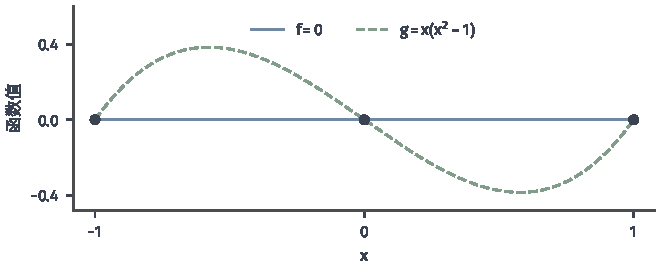
\includegraphics[width=112mm]{figures/00-shared/mathematical-preliminaries-upper/05-space-and-geometry/matplotlib/comprehension-additions/functional-unseen-observation-direction.pdf}
  \caption{有限点值留下不可见方向。定义域为$[-1,1]$，黑点为$x=-1,0,1$处的零读数。蓝线$f=0$与绿虚线$g(x)=x(x^2-1)$在三个位置完全一致，在其余位置可以不同。此处候选范围包含这些多项式；若另行限制次数或范数，仍须重新判断读取是否单射及候选是否可行。}
  \label{fig:vol1-add-functional-unseen-observation-direction}
\end{figure}

增加多项式次数、范数球或其他约束后，应在新的实际候选中重新检查哪些差函数仍可行：$g$不在新候选里，不可见方向就消失了。惩罚的作用是从同读数的多个函数中选定一个，它没有让原始数据获得额外识别能力——数据本身仍然看不见惩罚选定的方向。下一项用正交分解解释这种选择为什么能把搜索范围有限化。

\subsubsection{范数惩罚下的表示定理}
\label{subsubsec:representer-theorem}

\paragraph{用正交分解消去数据看不见的余项}

在实Hilbert空间$H$中取$n$个有界线性读取$L_i$。由第~\ref{subsubsec:riesz-representation}节的Riesz表示定理，每个$L_i$对应唯一方向$h_i\in H$使
\[
  L_i(f)=\langle f,h_i\rangle_H,\qquad i=1,\ldots,n.
\]
令
\[
  M=\operatorname{span}\{h_1,\ldots,h_n\}.
\]
$M$是有限维子空间；有限维子空间在Hilbert空间中闭（有限维空间上所有范数等价，柯西列必在该维数内收敛）。由第~\ref{subsubsec:orthogonal-projection}节的闭子空间投影结论，每个$f\in H$都有唯一正交分解
\[
  f=P_Mf+r,\qquad r\perp M,
\]
且$\|P_Mf\|_H\le\|f\|_H$。由$r\perp h_i$直接得到
\[
  L_i(r)=\langle r,h_i\rangle_H=0,\qquad i=1,\ldots,n,
\]
即余项$r$对全部读数不可见。这一步说明为什么去掉余项不改变数据项：不是“余项很小”，而是读数在$r$上恒为零。

现在考虑目标
\[
  J(f)=\Phi(Lf)+\Omega(\|f\|_H),
\]
其中$\Phi:\mathbb R^n\to\mathbb R$是读数代价，$\Omega:[0,\infty)\to\mathbb R$单调不减。因为$L_i(r)=0$，有$L(P_Mf)=Lf$，故$\Phi$两项相同；由$\|P_Mf\|_H\le\|f\|_H$及$\Omega$单调不减，得
\[
  J(P_Mf)=\Phi(Lf)+\Omega(\|P_Mf\|_H)
  \le\Phi(Lf)+\Omega(\|f\|_H)=J(f).
\]
于是在$M$中搜索与在全空间$H$中搜索取得相同下确界：任何$f$都被它的投影$P_Mf$（属于$M$）以不更差的目标取代。

\begin{theorem}[有限读取下的表示定理]\label{thm:functional-representer}
设$H$为实Hilbert空间，$L_1,\ldots,L_n$为有界线性读取，$h_i$为其Riesz方向，$M=\operatorname{span}\{h_i\}$。设
\[
  J(f)=\Phi(Lf)+\Omega(\|f\|_H),
\]
其中$\Phi$任意，$\Omega:[0,\infty)\to\mathbb R$单调不减。则：
\begin{enumerate}
  \item $\inf_{f\in H}J(f)=\inf_{f\in M}J(f)$；若$J$在$H$上达到最小值，则至少存在一个最小点属于$M$。
  \item 若$\Omega$还严格递增，且$J$达到最小值，则每个最小点都属于$M$。
  \item 若另有限制$C\subseteq H$代替全空间，上述结论在$P_M(C)\subseteq C$时成立；否则删除余项可能破坏可行性。
\end{enumerate}
\end{theorem}

\begin{proof}
对任意$f\in H$，上面已证$J(P_Mf)\le J(f)$且$P_Mf\in M$，故$\inf_{f\in M}J\ge\inf_{f\in H}J$，反向不等式由$M\subset H$直接得到，两端相等。若$f_*$是$H$上的最小点，则$J(P_Mf_*)\le J(f_*)$；又因$f_*$最小，$J(P_Mf_*)\ge J(f_*)$，故$P_Mf_*$也是最小点且属于$M$，本定理第一点成立。

若$\Omega$严格递增，且$f_*$的余项$r=f_*-P_Mf_*\ne0$，则$\|P_Mf_*\|<\|f_*\|$，由严格递增得$\Omega(\|P_Mf_*\|)<\Omega(\|f_*\|)$，从而$J(P_Mf_*)<J(f_*)$，与$f_*$最小矛盾；故$r=0$，即$f_*\in M$，本定理第二点成立。

有$C$限制时，$P_Mf$必须仍落在$C$中，上述投影取代才合法；第~3点的投影保持条件由此而来。
\end{proof}

注意定理没有说：下确界一定达到、最小函数唯一、或系数唯一。表示形式只是把搜索空间降到$M$，存在性与唯一性仍要由具体$\Phi,\Omega$另行判断。

\paragraph{惩罚含义与附加约束}

同为范数惩罚，$\Omega$所控制的对象由空间和范数的定义决定：$L^2$范数只累计函数值整体大小，整数阶Sobolev范数还累计规定阶弱导的整体大小，RKHS范数通过核截面同时控制点值稳定性和两点差，Lipschitz约束则直接限制函数随输入的变化幅度。不能笼统地把所有范数惩罚称为“让函数每点、每阶导数都同样平滑”。

点读取对应$h_i=K_{x_i}$（再生核截面，见第~\ref{subsubsec:point-evaluation}节），一般线性读取仍用各自的Riesz方向$h_i$；两者共用上面的证明，只是$h_i$的具体来源不同。附加约束方面，核范数球和仅依赖这组读数的约束可以逐项检查投影保持性$P_M(C)\subseteq C$，任意约束不可默认满足。完成这些条件后，才进入实际的有限参数目标。图~\ref{fig:representer-finite-readings-to-solver}把整个流程串起来。

\begin{figure*}[htbp]
  \centering
  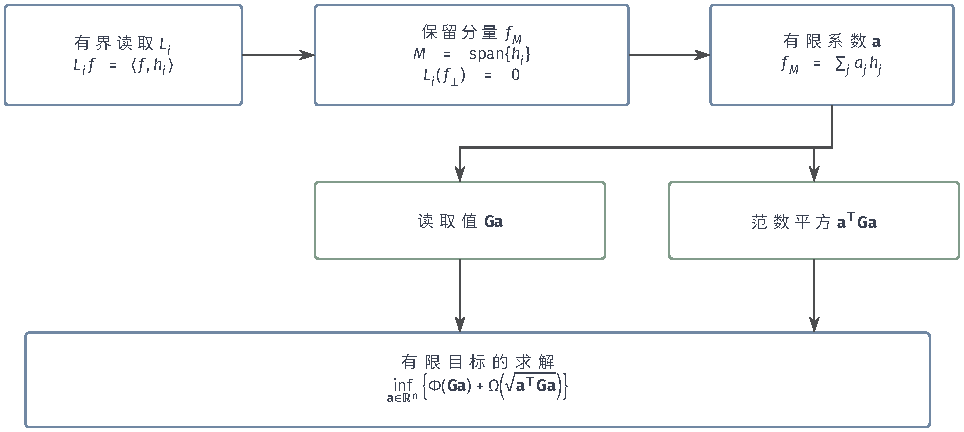
\includegraphics[width=163.258mm]{figures/00-shared/mathematical-preliminaries-upper/05-space-and-geometry/tikz/representer-finite-readings-to-solver/source.pdf}
  \caption{有限读取下的表示与求解。有界线性泛函$L_i$在Hilbert空间中有Riesz表示元$h_i$。所有读取只依赖$M=\operatorname{span}\{h_i\}$中的分量$f_M$，单调不减的范数惩罚允许删去$f_\perp$而不增大目标。写$f_M=\sum_j a_jh_j$后，读数与范数平方分别为$\bm G\bm a$与$\bm a^{\top}\bm G\bm a$。将这两个有限表达式代入目标后即可求解系数；最优解存在与系数唯一仍需另行判断。}
  \label{fig:representer-finite-readings-to-solver}
\end{figure*}

\subsubsection{Gram矩阵与平方拟合}
\label{subsubsec:gram-least-squares}

\paragraph{从函数目标到参数目标}

把$M$中的函数写成$f=\sum_{j=1}^n a_jh_j$，定义\term{Gram矩阵}
\[
  G_{ij}=\langle h_j,h_i\rangle_H=L_i(h_j),\qquad i,j=1,\ldots,n.
\]
逐项计算读数与范数：
\[
  (Lf)_i=L_i(f)=\sum_j a_jL_i(h_j)=\sum_jG_{ij}a_j,
\]
即$Lf=Ga$；以及
\begin{equation}
  \|f\|_H^2
  =\left\langle\sum_ja_jh_j,\sum_k a_kh_k\right\rangle_H
  =\sum_{i,j}a_iG_{ij}a_j=a^{\top}Ga.
  \label{eq:functional-finite-gram-objective}
\end{equation}
于是表示定理把目标化为有限变量$a\in\mathbb R^n$的问题：
\[
  \inf_{a\in\mathbb R^n}\left\{\Phi(Ga)+\Omega\!\left(\sqrt{a^{\top}Ga}\right)\right\}.
\]
只有读取恰好是点值$L_i(f)=f(x_i)$时，$G_{ij}=\langle K_{x_j},K_{x_i}\rangle_H=K(x_i,x_j)$才把$G$写成核矩阵；一般线性读取的Gram矩阵仍由$G_{ij}=\langle h_j,h_i\rangle$定义，不能省去“一般读数到核矩阵”这层条件。

取平方数据代价与二次范数惩罚，固定$\lambda>0$，考虑
\begin{equation}
  J_y(f)=\frac1n\sum_{i=1}^n(L_if-y_i)^2+\lambda\|f\|_H^2.
  \label{eq:functional-regularized-least-squares}
\end{equation}
代入有限表示$J_y(a)=\frac1n\|Ga-y\|_2^2+\lambda a^{\top}Ga$，对$a_j$求导：
\[
  \frac{\partial J_y}{\partial a_j}
  =\frac{2}{n}\sum_iG_{ij}(Ga-y)_i+2\lambda(Ga)_j.
\]
写成矩阵形式，驻点要求
\[
  \frac2nG(Ga-y)+2\lambda Ga=0,
\]
即
\[
  G\bigl[(G+n\lambda I)a-y\bigr]=0.
\]
注意$G$半正定：$a^{\top}Ga=\|\sum_ja_jh_j\|_H^2\ge0$。因此$G+n\lambda I$严格正定（其特征值为$t+n\lambda\ge n\lambda>0$），可逆。选取使括号内直接为零的规范代表
\begin{equation}
  a=(G+n\lambda I)^{-1}y.
  \label{eq:functional-tikhonov-representer}
\end{equation}
这里特意保留前一个驻点方程$G[(G+n\lambda I)a-y]=0$：后一个可逆方程只是选定代表，它要求括号向量本身为零；而驻点条件只要求该向量落在$\ker G$中，并未要求每组冗余系数都满足可逆方程。

为什么这个规范代表给出唯一的最优函数？先用前面已证的表示定理（定理~\ref{thm:functional-representer}）把搜索压到有限维。本问题的数据项$\Phi(z)=\frac1n\|z-y\|^2$凸，惩罚$\Omega(t)=\lambda t^2$随$t$严格递增；该定理已给出$\inf_{f\in H}J_y(f)=\inf_{f\in M}J_y(f)$，并且任何在$M$内达到下确界的点自动是$H$上的全局最小点。于是只需在$M$上证明最小值达到且唯一。

在$M$内写$f=\sum_ja_jh_j$，目标是系数$a\in\mathbb R^n$的二次函数$J_y(a)=\frac1n\|Ga-y\|^2+\lambda a^{\top}Ga$。把系数空间拆成$\ker G$与它的正交补：若$\delta a\in\ker G$，则$G\delta a=0$且$\delta a^{\top}G\delta a=0$，沿这个方向数据项与惩罚项都不变——系数冗余不改变函数，目标真正依赖的是$a$在$(\ker G)^\perp$上的投影$a_\perp$。退化情形先单独处理：若$\operatorname{rank}G=0$，则$G=0$；由$a^{\top}Ga=\|\sum_ja_jh_j\|_H^2$对一切$a$为零，迫使每个$h_i=0$，从而所有读数$L_if=\langle f,h_i\rangle\equiv0$恒为零，$M=\{0\}$。此时式~\eqref{eq:functional-regularized-least-squares}化为$J_y(f)=\frac1n\|y\|_2^2+\lambda\|f\|_H^2$，它随$\|f\|_H$严格增大，唯一最小点为$f_*=0$，最小代价为$\frac1n\|y\|_2^2$。以下设$\operatorname{rank}G\ge1$。在这个补空间上$G$严格正定：它是有限维对称矩阵，正特征值$t_i>0$全部出现，故有正的最小特征值$t_{\min}>0$。于是
\[
  J_y(a)\ge \lambda a_\perp^{\top}G a_\perp\ge \lambda t_{\min}\|a_\perp\|^2,
\]
右端随$\|a_\perp\|$增大而无界，目标在$(\ker G)^\perp$上强制。任取$c$，次水平集$\{a_\perp:J_y(a)\le c\}$一方面被$\|a_\perp\|\le\sqrt{c/(\lambda t_{\min})}$有界，另一方面是连续函数$J_y$的闭集；有限维闭且有界的集合必紧，由连续函数在紧集上达到极值的Weierstrass定理，$J_y$在$(\ker G)^\perp$上达到最小；$\ker G$方向任取零点，即得$M$上达到下确界的系数代表。

最后唯一性：数据项$\frac1n\|Lf-y\|^2$关于$f$凸，惩罚项$\lambda\|f\|_H^2$在$\lambda>0$时严格凸，故$J_y$在$H$上严格凸；严格凸函数至多有一个最小点，而最小点已在$M$内达到，故最小函数唯一。

\begin{theorem}[平方读取加二次惩罚的解]\label{thm:functional-tikhonov-solution}
设$H$为实Hilbert空间，$\lambda>0$，并给定$n$个有界线性读取
\[
  L_i:H\to\mathbb R,\qquad i=1,\ldots,n.
\]
则式~\eqref{eq:functional-regularized-least-squares}存在唯一的全局最小函数$f_*\in H$，且$f_*\in M=\operatorname{span}\{h_i\}$。其规范系数代表由式~\eqref{eq:functional-tikhonov-representer}给出：该代表在所有$h_i$方向满足一阶条件
\[
  DJ_y(f_*)[h_i]=0,
\]
在$M^\perp$方向上读数不变且$f_*$与扰动正交，一阶条件同样成立。
\end{theorem}

这里用具体二次目标完成了存在与唯一的证明，不能把这个结论反推给表示定理中任意的$\Phi,\Omega$。

\paragraph{函数唯一与系数冗余}

$G$奇异与最优函数唯一可以同时成立。若$\delta a\in\ker G$，则
\[
  \left\|\sum_j\delta a_jh_j\right\|_H^2
  =\delta a^{\top}G\,\delta a=0,
\]
由范数正定性，这个线性组合就是零函数；所有读数也都不变。因此问题不在函数层——最优函数唯一——而在坐标层：同一个函数$f_*=\sum_ja_j^*h_j$可以写成许多组系数，差向量都沿$\ker G$。

有附加约束时，先重查投影保持性$P_M(C)\subseteq C$，再把约束写成实际参数可行集。有限化只给出一个有限变量问题，不指定任何具体迭代算法都能收敛；下一项把“改变数据”和“增加计算次数”两种误差分别比较。

\subsubsection{数据扰动与计算误差}
\label{subsubsec:finite-fit-stability-computation}

\paragraph{固定惩罚参数时的数据稳定性}

固定$L_i,G,\lambda$，把观测数据从$y$改为$y+\delta y$，其余一切不动。规范代表的差为
\[
  \delta a=(G+n\lambda I)^{-1}\delta y.
\]
函数误差不能直接用系数欧氏距离$\|\delta a\|_2$计量——同一函数可有多组系数；正确的函数范数差是
\[
  \|\delta f\|_H^2=\delta a^{\top}G\,\delta a.
\]

把$G$正交对角化：$G=Q\operatorname{diag}(t_1,\ldots,t_n)Q^{\top}$，$t_i\ge0$。记$\tilde y=Q^{\top}\delta y$，则
\[
  \|\delta f\|_H^2
  =\sum_i\frac{t_i}{(t_i+n\lambda)^2}\,\tilde y_i^{\,2}.
\]
对每个$t\ge0$，由$(t+n\lambda)^2\ge4tn\lambda$（展开$t^2+2tn\lambda+n^2\lambda^2\ge4tn\lambda$即$(t-n\lambda)^2\ge0$）得
\[
  \frac{t}{(t+n\lambda)^2}\le\frac{1}{4n\lambda}.
\]
零特征方向$t=0$的权重为零，不贡献函数误差。合并得到
\begin{equation}
  \|\delta f\|_H\le\frac{\|\delta y\|_2}{2\sqrt{n\lambda}}.
  \label{eq:functional-data-stability-bound}
\end{equation}
这个界说明当前归一化$1/n$与固定的$\lambda$如何进入稳定常数。它比较的是两个不同数据任务的精确最优函数之差：没有研究任何求解算法，也没有让$\lambda$趋零。若随数据改变读取位置$x_i$或更换核，$G$本身也改变，就不能继续使用同一个矩阵逆的差分式~\eqref{eq:functional-tikhonov-representer}。

\paragraph{固定任务中的参数迭代}

现在固定同一数据目标$y$，只增加计算次数$k$。设迭代得到
\[
  f^{(k)}=\sum_i a_i^{(k)}h_i,
\]
最优规范代表为$a_*$。函数差的范数平方为
\[
  \|f^{(k)}-f_*\|_H^2
  =(a^{(k)}-a_*)^{\top}G(a^{(k)}-a_*).
\]
因此系数在$G$-内积意义下收敛足以推出函数收敛；有界读取再把函数收敛翻译成预测收敛。反向推断要小心：若$G$有零特征方向，系数沿$\ker G$改变时函数完全不变，所以“系数没怎么变”不保证函数没怎么变，“函数收敛”也不对应任何唯一的系数极限。因此停止条件必须说明检测的是参数、函数还是目标值。具体迭代算法的收敛仍需其光滑性、凸性和步长等条件，本节的表示定理不提供算法保证。

\subsection{整体函数值拟合}
\label{subsubsec:integral-error-fitting}

这里的数据不再是几个离散读数，而是整个定义域上的目标函数$y$：误差直接按积分范数在全体位置上累计。先处理Hilbert几何中“离目标最近的可行函数”这一纯几何问题，再处理RKHS候选与$L^2$观测之间的平方拟合；后者的解族极限和数据扰动放在同一任务内继续讨论，避免把不同范数、不同任务的结论分散使用。

\subsubsection{闭凸集合中的最近函数}
\label{subsubsec:nearest-closed-convex}

固定$f\in H$和非空闭凸集合$C\subset H$，研究
\[
  \inf_{g\in C}\|f-g\|_H.
\]
第~\ref{subsubsec:orthogonal-projection}节在闭子空间上证明过最近分量的存在唯一，那里$M$对线性组合封闭。现在$C$只是凸集，不再要求对线性组合封闭，但同一套估计仍然成立。

\paragraph{闭凸投影及其变分不等式}

\begin{theorem}[闭凸集上的最近点]\label{thm:functional-closed-convex-projection}
设$H$为实Hilbert空间，$C\subset H$非空闭凸。则存在唯一$g_*\in C$使$\|f-g_*\|_H=\inf_{g\in C}\|f-g\|_H$。
\end{theorem}

\begin{proof}
令$d=\inf_{g\in C}\|f-g\|_H$，取近似最小列$g_n\in C$使$\|f-g_n\|_H\to d$。凸性保证中点$(g_n+g_k)/2\in C$，故$\|f-(g_n+g_k)/2\|\ge d$。代入平行四边形恒等式
\[
  \begin{aligned}
    \|g_n-g_k\|^2
    &=2\|f-g_n\|^2+2\|f-g_k\|^2
      -4\left\|f-\frac{g_n+g_k}{2}\right\|^2\\
    &\le2\|f-g_n\|^2+2\|f-g_k\|^2-4d^2\to0,
  \end{aligned}
\]
$(g_n)$是柯西列。$H$完备给出极限$g_*$，$C$闭保留$g_*\in C$，范数连续性给出$\|f-g_*\|=d$。

若另有$g_{**}\in C$达到$d$，对它与$g_*$再用同一估计：
\[
  \|g_*-g_{**}\|^2
  \le2d^2+2d^2-4\left\|f-\frac{g_*+g_{**}}2\right\|^2
  \le4d^2-4d^2=0,
\]
故$g_*=g_{**}$。
\end{proof}

最近点$g_*$还可以用变分不等式刻画。沿可行方向$g_*+t(g-g_*)$（$0\le t\le1$，$g\in C$）展开：
\[
  \|f-g_*-t(g-g_*)\|^2
  =\|f-g_*\|^2-2t\langle f-g_*,g-g_*\rangle+t^2\|g-g_*\|^2.
\]
$t=0$是$t\ge0$上的最小，故一阶项非正：
\begin{equation}
  \langle f-g_*,g-g_*\rangle_H\le0,\qquad\forall g\in C.
  \label{eq:functional-convex-projection-characterization}
\end{equation}
反过来，若某个$g_*\in C$满足此不等式，则
\[
  \|f-g\|^2=\|f-g_*\|^2+\|g_*-g\|^2+2\langle f-g_*,g-g_*\rangle
  \ge\|f-g_*\|^2,
\]
故$g_*$确是最近点，条件充分。只有当$C$是闭线性子空间时，正负方向$g-g_*$都可行，不等式才加强为正交余项$\langle f-g_*,g\rangle=0$；一般凸集上只有单向变分不等式。

被最小化的整体误差由内积决定。若用Legendre、Chebyshev等方向作有限表示，区间变换的Jacobian及权重必须随内积重算；不能把换坐标后同一组系数的欧氏距离，当成原函数在$H$中的误差。

\subsubsection{RKHS平方拟合与谱收缩}
\label{subsubsec:rkhs-spectral-shrinkage}

\paragraph{明确两个空间并逐方向求解}

前面的最近点问题在单个Hilbert空间内进行。这里有两个空间：观测$y$在$L^2(\mu)$中累计，候选$f$在核Hilbert空间$H$中。沿用第~\ref{subsubsec:compact-spectrum-mercer}节给出的Mercer充分范围：紧度量输入域$X$、连续实对称半正定核$K$、有限正且全支撑的Borel测度$\mu$。在这些条件下，积分算子$T_K$在$L^2(\mu)$上紧自伴半正定，其归一特征方向$\psi_j$满足
\[
  T_K\psi_j=\mu_j\psi_j,\qquad \mu_j>0,
\]
且$\sqrt{\mu_j}\psi_j$构成$H$的完备正交系；$f=\sum_jb_j\psi_j\in H$当且仅当$\sum_jb_j^2/\mu_j<\infty$，且$\|f\|_H^2=\sum_jb_j^2/\mu_j$。固定该核的RKHS $H$与目标$y\in L^2(\mu)$，考虑
\begin{equation}
  J_\lambda(f)=\|f-y\|_{L^2(\mu)}^2+\lambda\|f\|_H^2,
  \qquad\lambda>0.
  \label{eq:functional-tikhonov-spectral-objective}
\end{equation}
$H\to L^2(\mu)$的有界性由再生关系和核对角上界$\sup_xK(x,x)<\infty$保证（紧集上连续核有界），两项积分因此都合法。只有当$\mu$总质量为一且相应观测解释成立时，才另外作统计解释；本节只作确定性拟合。

把$y$在$L^2(\mu)$中按$T_K$的谱分解：
\[
  y=y_0+\sum_jc_j\psi_j,\qquad y_0\in\ker T_K.
\]
对候选$f=\sum_jb_j\psi_j\in H$，$L^2$正交性把目标拆成互不耦合的方向：
\[
  J_\lambda(f)
  =\|y_0\|_{L^2}^2+\sum_j\left[(b_j-c_j)^2+\lambda\frac{b_j^2}{\mu_j}\right].
\]
零谱部分$y_0$没有可表示方向（$H$的元素只有正谱分量），它只贡献常数残差$\|y_0\|^2$；正谱部分则同时付出数据残差$(b_j-c_j)^2$与核范数代价$\lambda b_j^2/\mu_j$。

对每个正谱方向把括号配方：
\[
  (b_j-c_j)^2+\lambda\frac{b_j^2}{\mu_j}
  =\left(1+\frac{\lambda}{\mu_j}\right)
  \left(b_j-\frac{\mu_jc_j}{\mu_j+\lambda}\right)^2
  +\frac{\lambda c_j^2}{\mu_j+\lambda}.
\]
第一项系数$1+\lambda/\mu_j>0$，故逐方向唯一最小点为
\begin{equation}
  b_j^*=\frac{\mu_jc_j}{\mu_j+\lambda}.
  \label{eq:functional-spectral-shrinkage}
\end{equation}

这个式子目前只是形式候选：还要确认它确实给出$H$中的函数。由$\mu_j/(\mu_j+\lambda)^2\le1/(4\lambda)$（同一维均值不等式），
\[
  \sum_j\frac{(b_j^*)^2}{\mu_j}
  =\sum_j\frac{\mu_jc_j^2}{(\mu_j+\lambda)^2}
  \le\frac{1}{4\lambda}\sum_jc_j^2
  =\frac{\|y\|_{L^2}^2}{4\lambda}<\infty,
\]
故$f_*=\sum_jb_j^*\psi_j\in H$。目标值$\|y_0\|^2+\sum_j\lambda c_j^2/(\mu_j+\lambda)$是各项最小值之和，每个方向的配方都是严格凸二次，因此该候选达到唯一最小值。

\begin{theorem}[谱基下的正则化解]\label{thm:functional-spectral-shrinkage}
在上述Mercer范围与式~\eqref{eq:functional-tikhonov-spectral-objective}下，唯一最小函数为$f_*=\sum_j\frac{\mu_jc_j}{\mu_j+\lambda}\psi_j$，且$f_*\in H$。其$L^2$残差包含不可消除的零谱部分$\|y_0\|^2$。
\end{theorem}

\paragraph{表示误差与惩罚收缩}

回到仿射核算例核对方向。固定$X=[-1,1]$、$\mathrm d\mu=\mathrm dx/2$与$K(x,z)=1+xz$。第~\ref{subsubsec:compact-spectrum-mercer}节已算得归一方向$\psi_1=1$、$\psi_2=\sqrt3\,x$，正谱值$\mu_1=1$、$\mu_2=1/3$。收缩因子分别为
\[
  \frac{\mu_1}{\mu_1+\lambda}=\frac1{1+\lambda},
  \qquad
  \frac{\mu_2}{\mu_2+\lambda}=\frac{1/3}{1/3+\lambda}=\frac1{1+3\lambda},
\]
说明同一惩罚尺度$\lambda$对不同谱方向有不同收缩：小特征值方向被压得更狠。

取目标$y(x)=x^2$。它的正谱投影系数为
\[
  c_1=\langle x^2,\psi_1\rangle_{L^2(\mu)}=\int x^2\,\mathrm d\mu=\frac13,
  \qquad
  c_2=\langle x^2,\psi_2\rangle=\sqrt3\int x^3\,\mathrm d\mu=0,
\]
（$x^3$在对称区间积分为零），故$y=y_0+\frac13\psi_1$，$y_0=x^2-\frac13$。最优函数为
\[
  f_*=\frac{\mu_1c_1}{\mu_1+\lambda}\psi_1=\frac{1}{3(1+\lambda)}.
\]
零谱残差不可由任何$H$中函数表示：
\[
  \|y_0\|_{L^2}^2
  =\int\left(x^2-\frac13\right)^2\mathrm d\mu
  =\int x^4\,\mathrm d\mu-\frac23\int x^2\,\mathrm d\mu+\frac19
  =\frac15-\frac29+\frac19=\frac4{45}.
\]
另一类误差来自惩罚本身：$f_*$相对正谱投影$\frac13\psi_1$的收缩偏差为
\[
  \|f_*-\tfrac13\psi_1\|_{L^2}^2
  =\left(\frac{\lambda}{1+\lambda}\right)^2\frac19.
\]
表示残差$4/45$与收缩偏差不能合称为同一种拟合误差：前者由候选空间的谱覆盖不足造成，后者由惩罚选择造成。

令$\lambda=0$时，收缩消失，但$\sum_jc_j^2/\mu_j$可能发散，即正谱投影$P_+y$可能不属于$H$；此时下确界在$H$的闭包方向上达到，却没有$H$内最小函数。若另加范数球或额外点值约束，各方向系数将被新约束耦合，不能先逐方向收缩再默认它满足所有新约束。下一项在保持原任务条件时研究$\lambda$的解族。

\subsubsection{正则化参数的极限与有效维度}
\label{subsubsec:regularization-effective-dimension}

\paragraph{同一数据下的解族极限}

固定$y,K,\mu$，只改变$\lambda$，比较每个$\lambda$对应的精确解$f_\lambda$。由式~\eqref{eq:functional-spectral-shrinkage}，解相对正谱投影$P_+y=\sum_jc_j\psi_j$的$L^2$误差为
\[
  \|f_\lambda-P_+y\|_{L^2}^2
  =\sum_j\left(\frac{\lambda}{\mu_j+\lambda}\right)^2c_j^2.
\]
每一项随$\lambda\downarrow0$趋零，且被可求和的$\sum_jc_j^2=\|y\|^2_{L^2}$控制。按段取极限：先控制有限个前段（有限个数列逐项趋零），再用公共控制量$c_j^2$估计共同小的尾部（每一项$\le c_j^2$，尾和随$j$截断一致地小），取得
\[
  f_\lambda\to P_+y\quad\text{于 }L^2(\mu),\qquad\lambda\downarrow0.
\]
注意零谱残差$y_0$始终存在：$f_\lambda\to P_+y$而不是$y$，差$\|y_0\|$不可消除。

若正谱目标本身属于$H$，即$\sum_jc_j^2/\mu_j<\infty$，则在加权和中重复前段及尾部论证，可得$f_\lambda\to P_+y$于$H$范数。若该加权和发散，则
\[
  \|f_\lambda\|_H^2
  =\sum_j\frac{\mu_jc_j^2}{(\mu_j+\lambda)^2}
\]
随$\lambda\downarrow0$单调增至无穷（每项随$\lambda$减小而增大，由单调收敛定理取极限即$\sum_jc_j^2/\mu_j=\infty$）。此时只能在$L^2$范数下说$f_\lambda$收敛，不能写成$H$内收敛；这解释了“数据拟合越来越好”与“解的核范数爆炸”为何同时发生。

当$\lambda\to\infty$，各收缩系数$\mu_j/(\mu_j+\lambda)\to0$，且被原$c_j$一致控制，同样的级数估计给出$f_\lambda\to0$于$L^2$。这两端的参数极限比较的是“不同$\lambda$下各自的精确解”，与固定任务上的计算迭代无关。

\paragraph{给定惩罚尺度下的谱有效维度}

对固定$\lambda>0$，用
\begin{equation}
  d_{\mathrm{eff}}(\lambda)=\sum_j\frac{\mu_j}{\mu_j+\lambda}
  \label{eq:functional-effective-dimension}
\end{equation}
软计数被惩罚保留的方向：$\mu_j\gg\lambda$的方向贡献接近一，$\mu_j\ll\lambda$的方向贡献接近零。先检查这个级数是否有限：迹类条件$\sum_j\mu_j<\infty$给出上界
\[
  d_{\mathrm{eff}}(\lambda)\le\frac1\lambda\sum_j\mu_j.
\]
当前Mercer范围（连续核在紧集上）提供该条件：
\[
  \sum_j\mu_j=\int K(x,x)\,\mathrm d\mu(x)<\infty.
\]
仅有紧正算子还不够：例如特征值$\mu_j=1/j$的紧算子，$\sum_j\mu_j=\infty$，软计数级数同样发散。

仿射核在$\lambda=1$时给出
\[
  d_{\mathrm{eff}}(1)=\frac1{1+1}+\frac{1/3}{1/3+1}=\frac12+\frac14=\frac34,
\]
而其代数维数仍为二。\term{有效维度}是给定尺度$\lambda$下的谱量，不是函数类的覆盖规模：函数类覆盖还需另给函数类、半径和距离，二者都不独自提供统计或优化保证。图~\ref{fig:vol1-add-functional-effective-dimension}给出这个软计数的直观图像。

\begin{figure}[!htb]
  \centering
  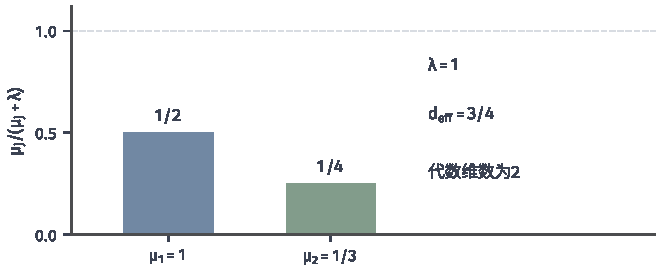
\includegraphics[width=112mm]{figures/00-shared/mathematical-preliminaries-upper/05-space-and-geometry/matplotlib/comprehension-additions/functional-effective-dimension-soft-count.pdf}
  \caption{有效维度按收缩比例计数。仿射核的两个正特征值为$1$和$1/3$，固定$\lambda=1$时，两个柱高分别为$1/(1+1)=1/2$与$(1/3)/(1/3+1)=1/4$，总和为$d_{\mathrm{eff}}=3/4$。灰虚线标记单一方向的完整贡献$1$，不表示另一项估计结果。}
  \label{fig:vol1-add-functional-effective-dimension}
\end{figure}

\subsubsection{固定参数下的数据稳定性}
\label{subsubsec:whole-fit-data-stability}

固定核、测度和$\lambda>0$，比较两个不同目标$y,\tilde y$对应的精确解$f_\lambda,\tilde f_\lambda$。对目标之差作相同的$L^2$谱分解：$y-\tilde y=\sum_j\delta c_j\psi_j$（零谱部分被消去），则解之差为
\[
  f_\lambda-\tilde f_\lambda=\sum_j\frac{\mu_j\delta c_j}{\mu_j+\lambda}\psi_j.
\]
按$L^2$范数计量，正谱系数乘上$\mu_j/(\mu_j+\lambda)\le1$，故
\[
  \|f_\lambda-\tilde f_\lambda\|_{L^2}
  \le\|y-\tilde y\|_{L^2}.
\]
这个结论比较同一算子的两项输入，$\lambda$全程固定，不让参数同时变化。

若按$H$范数计量输出，系数另带$1/\mu_j$权重：
\[
  \|f_\lambda-\tilde f_\lambda\|_H^2
  =\sum_j\frac{\mu_j\,\delta c_j^2}{(\mu_j+\lambda)^2}
  \le\frac{1}{4\lambda}\sum_j\delta c_j^2
  =\frac{\|y-\tilde y\|_{L^2}^2}{4\lambda},
\]
最后一步用$\mu_j/(\mu_j+\lambda)^2\le1/(4\lambda)$。于是
\begin{equation}
  \|f_\lambda-\tilde f_\lambda\|_H
  \le\frac{\|y-\tilde y\|_{L^2}}{2\sqrt\lambda}.
  \label{eq:functional-whole-fit-h-stability}
\end{equation}
换范数后常数从一变成$1/(2\sqrt\lambda)$，说明计量空间改变后实际改变了什么，而不是直接搬用前一段的系数一。

这里的数据稳定性、上一项的参数极限、以及有限任务中的算法误差各有各自的固定量与变化量：数据稳定性固定$K,\mu,\lambda$而改变$y$；参数极限固定$y,K,\mu$而改变$\lambda$；算法误差固定$y,K,\mu,\lambda$而增加迭代次数。一个任务既可能数据稳定又难以计算，也可能在$\lambda\downarrow0$时失去统一稳定常数，不能以其中一项代替另外两项。

\subsection{梯度场拟合与边界条件}
\label{subsubsec:gradient-field-fitting}

这里把观测从函数值改为向量场$v$：希望未知$u$的梯度接近$v$。固定有界连通Lipschitz域$\Omega\subset\mathbb R^d$，观测向量场$v\in L^2(\Omega;\mathbb R^d)$，已给提升$G\in H^1(\Omega)$与边界数据$g=\operatorname{Tr}G$（迹算子见第~\ref{subsubsec:trace-zero-boundary}节）。候选为
\[
  C=G+H_0^1(\Omega).
\]
残差是$\nabla u-v$；$v$未必是某个标量函数的精确梯度（例如环流场），因此不先假定残差可消为零，目标只能是“尽量小”。

\subsubsection{残差密度与可行扰动}
\label{subsubsec:residual-density-feasible}

在同一$v,g,C$上写残差密度的一般形式
\[
  J_\rho(u)=\int_\Omega\rho(\nabla u-v)\,\mathrm dx.
\]
二次密度$\rho_2(r)=\|r\|^2/2$与幅度型密度
\[
  \rho_\varepsilon(r)=\sqrt{\|r\|^2+\varepsilon^2}
\]
只改变残差的计价方式，不改变观测类型。它们可以与函数值项或有限读数项组合，但组合后必须重新写出完整目标、各项权重和共同候选，不能仅凭惩罚名称判断任务。

固定迹意味着允许扰动$h\in H_0^1(\Omega)$（边界迹为零）；若改为自由边界或均值约束，要先改变可行扰动集合，再使用共用的积分变分公式。$v=0$时上述两个密度才分别退化为纯梯度平方平滑与TV型平滑；没有其他观测或约束时，纯梯度平滑允许任意常量平移，不能说它自动保留信号。

\subsubsection{梯度残差的二次代价}
\label{subsubsec:quadratic-gradient-cost}

\paragraph{从二次目标到弱条件}

先取一维、$v=0$、固定端点的简单情形建立直觉：
\[
  J(f)=\frac12\int_0^1|f'|^2\,\mathrm dx.
\]
对光滑$f$和满足零端点条件的扰动$h$，展开
\[
  J(f+th)=\frac12\int|f'+th'|^2
  =J(f)+t\int f'h'\,\mathrm dx+\frac{t^2}{2}\int|h'|^2,
\]
故$DJ(f)[h]=\int f'h'\,\mathrm dx$。分部积分（$h$在端点为零，边界项消失）得$\int f'h'=-\int f''h$；由测试函数任意，驻点经典条件为$f''=0$，即仿射函数，再由固定端点值确定两个系数。一般$H^1$候选没有经典二阶导数时，先保留“对所有合法$h$成立”的积分条件$\int f'h'=0$，不强行点态化。注意这里是导数平方能量，要与二阶导数平方的弯曲能$\frac12\int|f''|^2$区别开：后者惩罚弯曲，前者惩罚斜率大小。

回到给定场$v\in L^2(\Omega;\mathbb R^d)$，取二次密度$\rho_2$（$v=0$时为$\frac12\int_\Omega\|\nabla u\|^2\,\mathrm dx$，即\term{Dirichlet能量}）：
\[
  J_2(u)=\frac12\int_\Omega\|\nabla u-v\|^2\,\mathrm dx.
\]
展开$J_2(u+th)-J_2(u)$的一次项（$h\in H_0^1$）：
\[
  t\int_\Omega(\nabla u-v)\cdot\nabla h\,\mathrm dx+o(t).
\]
故驻点弱式为
\begin{equation}
  \int_\Omega\nabla u\cdot\nabla h\,\mathrm dx
  =\int_\Omega v\cdot\nabla h\,\mathrm dx,
  \qquad\forall h\in H_0^1(\Omega).
  \label{eq:functional-guided-poisson-weak}
\end{equation}
当前$v\in L^2$和$u,h\in H^1$保证两边积分合法（Cauchy--Schwarz：$L^2$内$L^2$函数乘积可积）；即使$u$没有经典二阶导数，这个弱式仍保留。

在额外光滑条件下对左边分部积分，内部式解释为
\[
  \operatorname{div}(\nabla u-v)=0.
\]
自由边界处的自然通量是$(\nabla u-v)\cdot n$，一般不是齐次法向导数$\partial_nu=0$。若恰好$v=\nabla s$且$s\in H^1(\Omega)$，则$u-s$满足弱调和内部条件$\int\nabla(u-s)\cdot\nabla h=0$，边界差由修正项承担；任意$v$不必有这样的势$s$。

\paragraph{方程接口与求解边界}

这里的推导完成的是“候选与二次目标—可行一阶变化—弱方程”这条链路。带源Poisson方程、Poincaré不等式与Riesz表示下的存在唯一论证、自由边界的常量自由度以及源与通量相容条件，由后续微分方程章的Poisson弱解理论继续建立；本节不把当前驻点推导写成已经完成这些证明。连续弱问题存在唯一，也不能直接推出算法收敛或网格解逼近；具体五点系统及固定边界条件由五点差分承接，本章后面的连续能量离散节只检查已知函数的能量值和权重尺度，不替代解的数值分析。

\subsubsection{梯度残差的幅度代价}
\label{subsubsec:amplitude-gradient-cost}

\paragraph{正平滑参数下的一阶条件}

保留同一$v,g,C$，取$\varepsilon>0$及幅度型目标
\[
  J_\varepsilon(u)=\int_\Omega\sqrt{\|\nabla u-v\|^2+\varepsilon^2}\,\mathrm dx.
\]
先对残差向量$r=\nabla u-v$求密度导数：
\[
  \frac{\partial\rho_\varepsilon}{\partial r}
  =\frac{r}{\sqrt{\|r\|^2+\varepsilon^2}},
\]
再沿$\nabla h$用链式法则，得到一阶变化
\[
  \delta J_\varepsilon(u)[h]
  =\int_\Omega
  \frac{\nabla u-v}{\sqrt{\|\nabla u-v\|^2+\varepsilon^2}}
  \cdot\nabla h\,\mathrm dx.
\]
系数向量长度$\|\nabla u-v\|/\sqrt{\|\nabla u-v\|^2+\varepsilon^2}\le1$，被$|\nabla h|$一致支配，由控制收敛定理说明导数可以移入积分。令该一阶积分对全部合法$h\in H_0^1$为零，即得当前驻点弱条件；经典内部散度$\operatorname{div}\big((\nabla u-v)/\sqrt{\|\nabla u-v\|^2+\varepsilon^2}\big)=0$和自然边界通量，只在额外正则性或适用弱迹条件下解释。密度$\rho_\varepsilon$凸，故目标凸，但凸性不推出当前$H^1$候选中最小值达到或唯一，更不能沿用二次问题的Poisson线性形式。

\paragraph{零平滑参数、集中变化与BV边界}

当$\varepsilon=0$，残差为零处不能直接相除，应改用次梯度或变分不等式；$v=0$时密度退化为$\rho_0(r)=\|r\|$，即通常的\term{全变差}（TV）型平滑目标。用一个一维过渡比较两种密度对“集中变化”的响应：设$u$在宽度$\delta$内从高度$0$线性过渡到高度$a$，其余处斜率为零，则
\[
  \begin{aligned}
    \text{幅度积分}&=\int|u'|\,\mathrm dx=\frac{|a|}{\delta}\cdot\delta=|a|,\\
    \text{二次能量}&=\frac12\int|u'|^2\,\mathrm dx
      =\frac12\left(\frac a\delta\right)^2\delta=\frac{a^2}{2\delta}.
  \end{aligned}
\]
过渡收窄（$\delta\to0$）时幅度积分保持$|a|$不变，二次能量按$1/\delta$发散。二者对同一过渡的不同响应完全来自密度本身：幅度密度对“总变化量”计价，二次密度对“变化速率平方”计价。

一维中具有非零高度的跳跃不属于当前$H^1$候选（$H^1$函数在一维有绝对连续代表，不允许跳）。若要允许跳跃，必须以分布导数的测度表示进入BV空间并重新规定目标；本节只指出这条范围边界，不把BV存在理论混写成当前$H^1$结论。多维中逐坐标绝对值之和与逐点欧氏长度是不同密度，前者对方向的计价不同。即便密度逐点积分，共享的未知函数和边界约束仍耦合各位置，优化不能逐点独立；与其他观测项组合时，还须重新核对可微性、次梯度和可行保持条件。
\section{有限表示与函数逼近}
\label{sec:finite-representation-approximation}

本节固定目标函数、允许的定义域和误差尺度，研究怎样用有限个生成单元及其组合得到一个函数。前文的有限观测表示定理是在给定目标和惩罚下删除不可见方向；这里则主动选择近似族，并比较表示规模、局部修改和可达到的误差。“存在一个近似表示”只回答这个族是否足够丰富，不替代由有限读数识别目标、寻找参数的算法或学习保证。

下面固定一个共同目标
\[
  f_*(x)=\left|x-\frac12\right|,\qquad x\in[0,1],
\]
贯穿全节：多项式可以随次数增加而一致逼近它，含$1/2$结点的线性样条可以精确表示它，两个ReLU单元也可以精确表示它。这个对照比较的是同一个函数所需的构造条件，不从三个例子推断某种方案对所有目标都更省规模。生成单元的选择与多变量的组合方式是两个可以叠加的设计问题，下面分别讨论，不把它们写成互斥的函数类型。

\subsection{生成单元的选择}
\label{subsubsec:choice-of-generating-units}

下面固定同一个定义域与误差口径，分别考察全局多项式、局部分段直线、固定宽度的高斯核截面和神经单元怎样生成近似函数。四种方案各有自己的固定对象与可变规模：多项式的次数、样条的结点、高斯核的中心与项数、神经单元的宽度，分别随目标和精度变化，误差结论依赖的条件也随之不同。它们是几种有明确构造的方案，彼此可能存在表示联系；例如高斯核稠密性的证明借助多项式，却并不使高斯核截面成为多项式的一类。

\subsubsection{多项式逼近}
\label{subsubsec:polynomial-approximation}

对$[0,1]$上的连续目标$f$，先给一个可直接由网格读数形成的多项式，再证明它怎样控制全区间误差。结论中的次数可以随目标和精度增加，不固定一个有限维多项式空间后就宣称它能逼近所有连续函数。

在展开估计之前，先固定两个全程使用的对象。

\begin{definition}[连续模]
设$f$在区间$I$上有界。对$\delta>0$，定义
\[
  \omega_f(\delta)=\sup_{\substack{s,t\in I\\|s-t|\le\delta}}|f(s)-f(t)|.
\]
它是$f$在长度$\delta$的尺度上的最大振幅。$f$在紧区间上一致连续，等价于$\omega_f(\delta)\to0$（$\delta\downarrow0$）；若$f$还满足$|f(s)-f(t)|\le L|s-t|$，则有$\omega_f(\delta)\le L\delta$。
\label{def:functional-continuity-modulus}
\end{definition}

\paragraph{Bernstein多项式的构造}

固定整数$m\ge1$，在结点$j/m$读取$f$，定义
\begin{equation}
  B_mf(x)=\sum_{j=0}^{m}f\!\left(\frac jm\right)w_{m,j}(x),
  \qquad
  w_{m,j}(x)=\binom mjx^j(1-x)^{m-j}.
  \label{eq:functional-bernstein-polynomial}
\end{equation}
结点值是已知输入，$x$是求近似值的位置；每个权重都是$x$的多项式，因此结果仍是次数至多$m$的多项式。

把$m$个$x+(1-x)$的有限乘积按“选中$x$的次数”分组，得到
\[
  \sum_jw_{m,j}(x)=\bigl(x+(1-x)\bigr)^m=1;
\]
在$0\le x\le1$上各权重非负，因此$B_mf(x)$是结点值的凸组合。这一步只用有限乘积和二项式展开，不预先调用概率论。凸组合说明了取值范围，却还没有说明主要权重是否集中在靠近$x$的结点；下面把这个位置问题算成一组有限和恒等式。

\begin{lemma}[Bernstein权重的矩]
对$0\le x\le1$，上述权重满足
\[
  \sum_{j=0}^m w_{m,j}(x)=1,\qquad
  \sum_{j=0}^m j\,w_{m,j}(x)=mx,
\]
以及
\[
  \sum_{j=0}^m j(j-1)w_{m,j}(x)=m(m-1)x^2.
\]
进而有二阶中心矩恒等式
\begin{equation}
  \sum_{j=0}^m\left(\frac jm-x\right)^2w_{m,j}(x)
  =\frac{x(1-x)}m\le\frac1{4m}.
  \label{eq:functional-bernstein-second-moment}
\end{equation}
\end{lemma}

\begin{proof}
第一式已由二项式定理给出。对第二式，利用$j\binom mj=m\binom{m-1}{j-1}$，把求和下标改为$k=j-1$：
\[
  \sum_{j=0}^m j\,w_{m,j}(x)
  =mx\sum_{k=0}^{m-1}\binom{m-1}{k}x^k(1-x)^{m-1-k}
  =mx.
\]
对第三式，再用$j(j-1)\binom mj=m(m-1)\binom{m-2}{j-2}$（$m=1$时左边直接为零），类似地把下标改为$k=j-2$，得到
\[
  \begin{aligned}
  \sum_{j=0}^m j(j-1)w_{m,j}(x)
  &=m(m-1)x^2
    \sum_{k=0}^{m-2}\binom{m-2}{k}x^k(1-x)^{m-2-k}\\
  &=m(m-1)x^2.
  \end{aligned}
\]
最后用$j^2=j(j-1)+j$展开二阶中心矩：
\[
  \sum_j(j/m-x)^2w_{m,j}
  =\frac1{m^2}\sum_jj^2w_{m,j}-\frac{2x}{m}\sum_jj\,w_{m,j}+x^2\sum_jw_{m,j}.
\]
代入前两式，即得$(m(m-1)x^2+mx)/m^2-2x^2+x^2=x(1-x)/m$；再由$x(1-x)\le1/4$（$0\le x\le1$）得到右端上界$1/(4m)$。
\end{proof}

这个有限和恒等式的意义是：权重虽然散布在全部结点上，但离$x$较远的结点所占的总权重受$1/(4m)$控制，因而随$m$增大而衰减。

\paragraph{一致误差的估计}

\begin{theorem}[Bernstein--Weierstrass逼近]
设$f\in C([0,1])$，$B_mf$为式~\eqref{eq:functional-bernstein-polynomial}的Bernstein多项式。对任意$\delta>0$，
\begin{equation}
  \|B_mf-f\|_\infty
  \le\omega_f(\delta)+\frac{\|f\|_\infty}{2m\delta^2}.
  \label{eq:functional-bernstein-error}
\end{equation}
因而$\|B_mf-f\|_\infty\to0$（$m\to\infty$）。
\end{theorem}

\begin{proof}
固定$\delta>0$，用权重和为一把差写成
\[
  B_mf(x)-f(x)
  =\sum_{j=0}^m\left[f\!\left(\frac jm\right)-f(x)\right]w_{m,j}(x).
\]
把结点分成近处$|j/m-x|\le\delta$与远处$|j/m-x|>\delta$两组，这是同一个误差的两部分，并未另换目标或误差范数。

近处每个差值至多为连续模$\omega_f(\delta)$，而近处权重之和不超过$1$，故近处贡献不超过$\omega_f(\delta)$。

远处对每个$j$用$1\le(j/m-x)^2/\delta^2$放大权重，再由上面的矩恒等式控制总权重：
\[
  \sum_{|j/m-x|>\delta}w_{m,j}(x)
  \le\frac1{\delta^2}\sum_{j=0}^m\left(\frac jm-x\right)^2w_{m,j}(x)
  \le\frac1{4m\delta^2}.
\]
远处再用$|f(j/m)-f(x)|\le|f(j/m)|+|f(x)|\le2\|f\|_\infty$，得到远处贡献不超过$\|f\|_\infty/(2m\delta^2)$。两部分相加即得式~\eqref{eq:functional-bernstein-error}。

最后，$f$在紧区间$[0,1]$上一致连续，故任给$\varepsilon>0$可先选$\delta$使$\omega_f(\delta)<\varepsilon/2$；保持这个$\delta$，再取足够大的$m$使$\|f\|_\infty/(2m\delta^2)<\varepsilon/2$。两步缺一不可：仅知道某个固定$x$处误差趋零，不足以得出全区间共用的结论。
\end{proof}

回到折点目标$f_*$，本定理保证任意精度的一致多项式逼近，但任意一个多项式在$1/2$处都可微，不能与$f_*$在整个区间上完全相同。一般连续性也没有给出所有连续目标共用的快速速率；上面的速率$\omega_f(\delta)+C/(m\delta^2)$只说明收敛，常数随$\delta$的选择而变。下一个方案利用分段结构，在特定结点条件下直接表示这个折点。

\subsubsection{样条逼近}
\label{subsubsec:spline-approximation}

样条以分段多项式和指定结点衔接条件定义。这里先取最简单的连续分段直线，研究结点值怎样生成局部插值，以及结点变密怎样控制同一个连续目标的误差。

\paragraph{线性样条的构造与误差}

固定
\[
  0=t_0<t_1<\cdots<t_N=1,
\]
结点值$f(t_i)$及最大间距$h=\max_i(t_{i+1}-t_i)$。对$x\in[t_i,t_{i+1}]$写
\begin{equation}
  S_hf(x)=(1-s)f(t_i)+sf(t_{i+1}),
  \qquad s=\frac{x-t_i}{t_{i+1}-t_i}.
  \label{eq:functional-linear-spline}
\end{equation}
相邻区间在公共结点使用同一个读数，所以这个构造给出连续分段直线。要先区分“由全部样条组成的候选空间”与“由结点数据产生当前插值函数的操作”。

\begin{theorem}[线性样条的插值误差]
在上述记号下，若$f$在$[0,1]$上连续，则
\begin{equation}
  \|f-S_hf\|_\infty\le\omega_f(h).
  \label{eq:functional-spline-modulus-error}
\end{equation}
若再有$f\in C^2([0,1])$，则
\begin{equation}
  \|f-S_hf\|_\infty\le\frac{h^2}{8}\|f''\|_\infty.
  \label{eq:functional-spline-quadratic-error}
\end{equation}
\end{theorem}

\begin{proof}
在单元$[t_i,t_{i+1}]$上，由$(1-s)+s=1$把$f(x)-S_hf(x)$拆成
\[
  f(x)-S_hf(x)=(1-s)\bigl(f(x)-f(t_i)\bigr)+s\bigl(f(x)-f(t_{i+1})\bigr).
\]
两个端点离$x$都不超过$h$：$|x-t_i|=s(t_{i+1}-t_i)\le h$，$|x-t_{i+1}|=(1-s)(t_{i+1}-t_i)\le h$。故
\[
  |f(x)-S_hf(x)|\le(1-s)\omega_f(h)+s\omega_f(h)=\omega_f(h).
\]
对全部区间取上确界即得式~\eqref{eq:functional-spline-modulus-error}。若一列网格的最大间距$h\to0$，一致连续性使$\omega_f(h)\to0$，这些插值函数便一致趋于$f$；这个结论不要求网格等距。

为得到二阶速率，固定一个单元并考虑$g(x)=f(x)-S_hf(x)$。它在两端$t_i,t_{i+1}$处为零。对任意$x\in(t_i,t_{i+1})$，令
\[
  \lambda=\frac{g(x)}{(x-t_i)(x-t_{i+1})},
  \qquad
  G(u)=g(u)-\lambda(u-t_i)(u-t_{i+1}).
\]
函数$G$在$t_i,t_{i+1},x$三点处都为零。由Rolle定理，$G'$在这三点两两之间各有一个零点，共两个零点；再用一次Rolle定理，$G''$在单元内某点$\xi$处为零。注意$S_hf$在单元内是一次多项式，$S_h''=0$，而$((u-t_i)(u-t_{i+1}))''=2$，故
\[
  0=G''(\xi)=f''(\xi)-2\lambda,
  \qquad
  \lambda=\frac{f''(\xi)}2.
\]
代回$\lambda$的定义，得余项表示
\[
  f(x)-S_hf(x)=\frac{f''(\xi)}2(x-t_i)(x-t_{i+1}).
\]
在单元上$|(x-t_i)(x-t_{i+1})|\le\bigl((t_{i+1}-t_i)/2\bigr)^2\le h^2/4$，因而$|f(x)-S_hf(x)|\le h^2\|f''\|_\infty/8$。对单元取上确界即得式~\eqref{eq:functional-spline-quadratic-error}。新增的二阶导数条件支持更具体的速率，不能由一般连续性直接取得。
\end{proof}

\paragraph{样条的示例与局部修改}

\begin{example}[二次函数的两段插值]
对$f(x)=x^2$只取结点$0,1$，由端点值$0,1$得到$S_hf(x)=x$。函数$x-x^2$在$x=1/2$处取最大值$1/4$，故误差恰为$1/4$。此时$h=1$、$\|f''\|_\infty=2$，上一界$h^2\|f''\|_\infty/8=2/8=1/4$，二者吻合，可供核对余项估计中的常数。
\end{example}

对折点目标$f_*$，若结点包含$0,1/2,1$，则$[0,1/2]$上的直线斜率为$-1$、$[1/2,1]$上的斜率为$+1$，与$f_*$两侧斜率相同，因此已能精确表示。它与多项式方案比较的是同一目标在不同生成规则下的表示条件，并不说明某个固定结点集合能精确表示任意连续目标。

固定其他结点值、只改变一个内部结点的值时，当前线性插值公式只在相邻两段改变，这种局部性来自帽形生成函数的支撑；误差界则来自端点凸组合，两种结论使用不同依据。图~\ref{fig:functional-basis-locality}把三类生成单元在同一结点$1/2$处取单位系数放在一起比较，可见局部支撑与全局基的差别。提高样条次数或改成多变量张量积后，要重新检查衔接、插值与系数依赖，不能把“局部分段”直接当成全部性质的保证。

\begin{center}
\begin{minipage}{\linewidth}
 \centering
 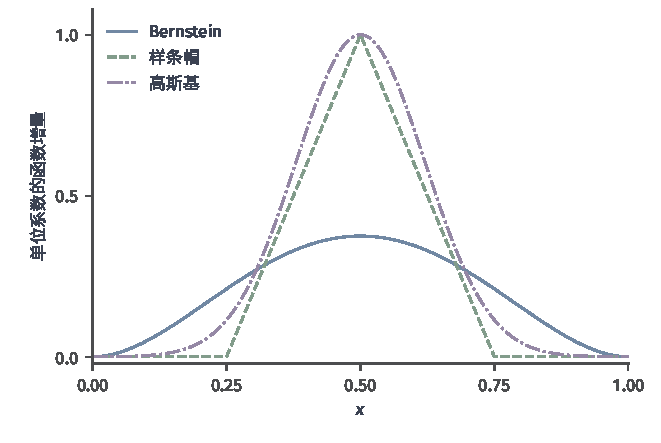
\includegraphics[width=112mm]{figures/00-shared/mathematical-preliminaries-upper/05-space-and-geometry/matplotlib/teaching-analysis/functional-basis-locality.pdf}
 \functionalinlinefigurecaption{fig:functional-basis-locality}
   {同一结点$1/2$处取单位系数的三类生成单元。Bernstein权重（实线）在整个$(0,1)$上非零，峰值远小于$1$；线性样条帽形函数（虚线）只在相邻两段$[1/4,3/4]$上非零，即局部支撑；高斯核截面（点划线）光滑衰减但处处非零。改变一个内部结点值只影响帽形基所在两段插值，这种局部性来自生成函数的支撑，与插值误差的凸组合界依据不同；全局基的系数依赖范围也随之更宽。}
\end{minipage}
\end{center}

\subsubsection{固定宽度高斯核截面的逼近}
\label{subsubsec:gaussian-section-approximation}

现在保持每个生成单元的宽度不变，只允许中心、线性系数和项数变化。要证明这套单元也能逼近连续目标，需要把核截面的有限和与前面的多项式逼近联系起来；证明中借助多项式，但所得近似器仍是高斯核截面的有限和。

\paragraph{固定宽度的核截面与中心差分}

在$[0,1]$固定$\sigma>0$，取
\[
  K_\sigma(x,c)=\exp\left(-\frac{(x-c)^2}{2\sigma^2}\right),
\]
并允许所有中心$c\in[0,1]$。候选近似器为
\[
  \sum_{\ell=1}^{M}a_\ell K_\sigma(\cdot,c_\ell),
\]
其中$M$和实系数可以变化；这里的稠密性采用一致范数，不对系数大小或核空间范数预设统一预算。

固定内部中心$c_0=1/2$，令$w(x)=K_\sigma(x,c_0)$。对中心连续求导：一阶导数为$\partial_cK_\sigma(x,c)=(x-c)K_\sigma(x,c)/\sigma^2$，它仍含因子$w(x)$；逐次求导便归纳地得到
\begin{equation}
  \partial_c^jK_\sigma(x,c_0)=w(x)P_j(x),
  \label{eq:functional-gaussian-derivative-polynomial}
\end{equation}
其中$P_j$是次数$j$的多项式，最高次项系数为$\sigma^{-2j}$。归纳步骤是：对$w(x)P_j(x)$再关于$c$求一次导，新增项$(x-c)wP_j/\sigma^2$只把最高次数提高一次，且首项系数乘$\sigma^{-2}$。

对每个固定$j$，取足够小的$h>0$，使$c_0,c_0+h,\ldots,c_0+jh$都在合法中心域内，写中心$j$阶前向差分
\begin{equation}
  h^{-j}\sum_{\ell=0}^{j}(-1)^{j-\ell}\binom j\ell
  K_\sigma(x,c_0+\ell h).
  \label{eq:functional-center-forward-difference}
\end{equation}
这是$j$个核截面的有限线性组合。由$\partial_c^jK_\sigma$在紧矩形$[0,1]\times[c_0-\varepsilon,c_0+j\varepsilon]$上连续，有限差分对全部$x$一致收敛到导数~\eqref{eq:functional-gaussian-derivative-polynomial}。因此每个$wP_j$都属于核截面有限和的一致闭包；不能只从逐点求导就直接宣称一致逼近，一致性来自差分在$x$上的一致收敛。

\paragraph{从加权多项式到一致稠密性}

\begin{theorem}[固定宽度高斯核截面的一致稠密性]
设$\sigma>0$固定，则全体有限和$\sum_{\ell=1}^{M}a_\ell K_\sigma(\cdot,c_\ell)$（$M$、$a_\ell$、$c_\ell$均可随目标变化）在$C([0,1])$的一致范数下稠密。
\end{theorem}

\begin{proof}
分三步。

第一步，把多项式方向并入闭包。$P_j$的最高次项非零（系数$\sigma^{-2j}\ne0$），故$P_0,P_1,\ldots,P_m$与单项式$1,x,\ldots,x^m$之间的系数变换是对角元非零的上三角变换。逐次消去最高次数，就能把任意次数至多$m$的多项式$P$写成$P_0,\ldots,P_m$的有限线性组合。于是每个加权多项式$wP$也属于核截面有限和的一致闭包。

第二步，把目标折成加权多项式。$w$在紧区间$[0,1]$上连续且严格为正，故有正下界；$f$连续时$f/w$仍连续。对$f/w$用已证明的Bernstein--Weierstrass定理，可找多项式$P$使$\|f/w-P\|_\infty$任意小，即$\|f-wP\|_\infty$任意小。

第三步，把$wP$换成真正的有限核和。把$P=\sum_j c_jP_j$写成有限组合；对每个固定$j$，由中心差分~\eqref{eq:functional-center-forward-difference}选足够小的步长，使该$wP_j$的一致逼近误差任意小。最后用三角不等式合并“$f$到$wP$”与“$wP$到有限核和”两类误差，便得到一个项数有限的高斯核截面和，其一致误差小于任意给定精度。
\end{proof}

项数和中心可以随目标及精度变化，是上述结论的条件。若只允许一个预先固定的有限中心集合，所得有限维张成在$C([0,1])$中是闭的且不等于整个空间，便不具有这种稠密性；差分中的小步长还可能带来大系数，证明不提供统一的规模、数值稳定或寻参保证。固定宽度高斯核在紧集上的通用性可与Steinwart的原论文核对\scite{steinwart2001kernel}；这里展开的是一维区间上的具体证明路线。

\subsubsection{神经网络逼近}
\label{subsubsec:neural-network-approximation}

神经单元把输入的仿射变换送入激活函数，再由有限线性组合形成输出。先对共同折点目标直接计算，再区分这个小构造与“对所有连续目标”的存在定理。

\paragraph{折点函数的两单元表示}

\begin{example}[折点函数的两ReLU表示]
定义$\operatorname{ReLU}(s)=\max(s,0)$。对$f_*(x)=|x-1/2|$，直接写
\[
  \operatorname{ReLU}\!\left(x-\frac12\right)
  +\operatorname{ReLU}\!\left(\frac12-x\right).
\]
当$x\ge1/2$时第一项为$x-1/2$、第二项为零；当$x\le1/2$时第一项为零、第二项为$1/2-x$；两端合并恰为$|x-1/2|$。分两侧核对后可见：两个输入权重取正负号、偏置都放在折点$1/2$、输出相加，各自的作用都不可省略。
\end{example}

这个单隐藏层构造使用两个ReLU单元，不要求训练过程就能验证其表示。它与线性样条共用同一折点目标是为了比较生成规则；一个简单函数有小网络，并不推出任意目标都有同样规模，也不由两侧计算推出通用逼近定理。

\paragraph{通用逼近的条件与边界}

\begin{theorem}[单隐藏层通用逼近]
固定非空紧集$X\subset\mathbb R^d$、$f\in C(X)$和连续且不是多项式的激活函数$\sigma$。采用含偏置的单隐藏层形式
\begin{equation}
  c+\sum_{j=1}^{M}a_j\sigma(w_j^{\top}x+b_j).
  \label{eq:functional-universal-approximation}
\end{equation}
则对每个$\varepsilon>0$，可以选择有限的$M$与实参数$c,a_j,w_j,b_j$，使式~\eqref{eq:functional-universal-approximation}在$X$上与$f$的一致误差小于$\varepsilon$。
\end{theorem}

这一连续激活版本由Leshno等人的结果支持\scite{leshno1993approximation}；这里陈述的是存在定理，不伪装成已经给出针对一般目标的构造算法。

用Sigmoid、Tanh和ReLU核对“连续且非多项式”的条件，可知定理不要求激活处处可微。反之，若激活是固定次数$r$的多项式，同一单隐藏层形式无论增加多少单元：仿射变换$w_j^\top x+b_j$代入$r$次多项式后仍是次数至多$r$的多项式，有限线性组合后输出次数仍至多$r$。这种固定次数空间不能在有非空内部的紧域上逼近所有连续目标（例如$x^{r+1}$在一个小区间上的行为）。因此“用了非线性”不足以替代非多项式条件，偏置也属于这里采用的定理形式。

一致误差控制全部输入位置；转为$L^2(\mu)$误差时，还要给出测度及有限总质量，才能使用
\[
  \|f-g\|_2=\left(\int_X|f-g|^2\,\mathrm d\mu\right)^{1/2}
  \le\mu(X)^{1/2}\|f-g\|_\infty.
\]
反向可能受小区域尖峰阻碍：$L^2$小而一致误差大的函数对是存在的。由评价对象不同可以说明两个逼近命题的联系与边界，同时保留这些限制：通用逼近不保证最小宽度、参数可由有限读数识别、训练收敛或泛化。

\subsection{多变量函数的组合}
\label{subsubsec:multivariable-composition}

输入分为$p,q$两组后，可以把单组函数组合成有限乘积和
\[
  F_r(p,q)=\sum_{j=1}^{r}u_j(p)v_j(q);
\]
多项式、样条或神经单元都可作为因子的构造方式。这里研究的是变量如何共同作用，改变了上一分支中“只选生成单元”的问题；项数$r$与因子幅度仍须分别记录。

下面按实际任务区分：已给整个目标函数时，构造分离近似并控制全域误差；已给规则网格读数时，构造符合这些读数的\term{张量积插值}。两者不是互斥的结构类型，网格系数也可以具有低秩；“没有指定网格读数”不是低秩的定义。先确定共同乘积结构，再说明各任务额外固定的数据和评价条件。

\subsubsection{给定函数的分离近似}
\label{subsubsec:separated-approximation}

固定整个二维目标后，问少量单组因子的乘积之和能否在整个定义域上控制误差。所构造的项数给出一个可行表示规模，不自动给出所有同规模表示中的最优误差。

\paragraph{指数函数的分离构造}

固定$E(p,q)=e^{pq}$及$(p,q)\in[-1,1]^2$，取
\begin{equation}
  E_r(p,q)=\sum_{k=0}^{r-1}\frac{p^kq^k}{k!}.
  \label{eq:functional-separated-taylor}
\end{equation}
逐项写成只依赖$p$的$p^k/k!$与只依赖$q$的$q^k$的乘积；这个Taylor构造因此使用至多$r$个分离项，不能只因它写成一个二维多项式，就跳过变量分组的识别。

因$|pq|\le1$，把$pq$看作一元变量$t$，一元指数Taylor余项给出
\[
  |e^{pq}-E_r(p,q)|\le\frac{e^{|pq|}|pq|^r}{r!}\le\frac{e}{r!}.
\]
对整个正方形取上确界后仍有相同上界，故增加项数给出一致逼近；这是一条可行截断序列的保证，并未证明它在所有$r$项分离表示中最优。

再固定$q=1$观察$r=1,2,4$：对应截面分别为$1$、$1+p$、$1+p+p^2/2+p^3/6$，在$p=1$处的误差可直接核对为$e-1$、$e-2$和$e-8/3$（即$e-8/3\approx0.052$）。这些截面与具体点值帮助解释展开过程，整个定义域上的保证仍由上一段余项估计给出。图~\ref{fig:vol1-add-functional-separated-taylor-remainder}沿$q=1$截面展示余项，不要求读者另看图片才理解界。

\begin{figure}[!htb]
  \centering
  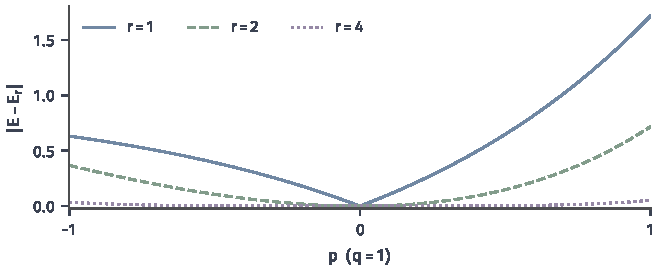
\includegraphics[width=112mm]{figures/00-shared/mathematical-preliminaries-upper/05-space-and-geometry/matplotlib/comprehension-additions/functional-separated-taylor-remainder.pdf}
  \caption{分离表示的截断余项。目标为$E(p,q)=e^{pq}$，$E_r$保留$k=0,\ldots,r-1$共$r$项，图中固定$q=1$并比较$r=1,2,4$的绝对误差$|E-E_r|$；三条曲线在$p=0$处均为零，随$|p|$增大而上升，$r$越大误差越小。所有曲线由解析式计算。正文界$e/r!$对整个$[-1,1]^2$成立；这里没有声称Taylor截断是最佳秩$r$逼近。}
  \label{fig:vol1-add-functional-separated-taylor-remainder}
\end{figure}

\paragraph{分离项的尺度与适用范围}

把$r$个因子分别组成向量$u(p)$与$v(q)$，其第$j$个分量为$u_j(p)$与$v_j(q)$，由Cauchy--Schwarz得
\[
  |F_r(p,q)|=\left|\sum_{j=1}^ru_j(p)v_j(q)\right|
  \le\|u(p)\|_2\|v(q)\|_2.
\]
项数说明表示用了多少个分离方向，因子范数控制这些方向的幅度；相同项数并不限制输出大小，也不独自控制函数类在指定误差下的覆盖数。某些Bellman残差矩阵也使用两个因子内积的形式，可据此辨认结构上的类比；但矩阵条目的含义、可实现性、查询协议与样本结论都依赖相应决策任务。这里不从$e^{pq}$的Taylor误差或一般因子界推出强化学习保证，函数类的统一代表数量留给覆盖数任务另行定义。

\subsubsection{网格数据的张量积插值}
\label{subsubsec:tensor-grid-interpolation}

现在不预先给出整个目标，只固定单位整数网格上的样本值$U_{ij}$，希望在非整数位置求值且经过原有网格读数。共同形式是
\begin{equation}
  S(x,y)=\sum_{i,j}c_{ij}h(x-i)h(y-j);
  \label{eq:functional-tensor-interpolation}
\end{equation}
一维核决定每轴的衔接与支撑，系数如何由样本产生则是另一项必须核对的条件。有限网格须指定边界延拓；下面B样条的可逆论证明确采用周期边界，不能自动移给其他端点条件。

三种方案在同一任务下比较结点插值、导数连续、取值范围和计算依赖：双线性和三次卷积可以直接用样本作系数；三次B样条则要先恢复系数再局部求值。这个差别在选择局部核时就必须注意，不能以“都具有有限支撑”掩盖样本到系数的过程。

\paragraph{双线性插值}

定义帽核$h(s)=\max(1-|s|,0)$，核对$h(0)=1$、非零整数处为零（基数条件）。取$c_{ij}=U_{ij}$时，整数网格位置$(i,j)$只留下对应的一个样本$U_{ij}$，因此满足插值；二维形式由两轴核的乘积生成。

对查询$(x,y)=(i+s,j+t)$、$s,t\in[0,1]$，只有四个核同时非零，展开权重
\[
  (1-s)(1-t),\quad s(1-t),\quad (1-s)t,\quad st
\]
及其对应四角样本$U_{i,j},U_{i+1,j},U_{i,j+1},U_{i+1,j+1}$。每项非负且总和为一，所以输出落在这四个样本的最小值和最大值之间；范围保持来自凸组合，而非来自“线性”这个名称。固定一个坐标时输出关于另一坐标线性；共同展开一般含$st$交叉项，所以通常不是整个平面上的仿射函数。相邻单元在公共边使用同一线性插值，函数值能够衔接，一阶导数一般会跳变；这也明确了更换核所要改善的是哪一种连续性。给定边界延拓后，每次求值只用所在单元四角样本，也可先沿一轴再沿另一轴计算。

\paragraph{三次卷积插值}

令$r=|s|$，定义Keys核：
\[
  h_a(s)=
  \begin{cases}
    (a+2)r^3-(a+3)r^2+1,&0\le r\le1,\\
    ar^3-5ar^2+8ar-4a,&1<r<2,\\
    0,&r\ge2.
  \end{cases}
\]
先检查衔接：$r=1$处左段值$(a+2)-(a+3)+1=0$、右段值$a-5a+8a-4a=0$，两侧一阶导数分别为$3(a+2)-2(a+3)=a$与$3a-10a+8a=a$，故函数值与一阶导数都连续；$r=2$处右段值$8a-20a+16a-4a=0$、导数$12a-20a+8a=0$，与外侧零相接；原点处两段关于$|s|$对称。综合得到$C^1$衔接和有限支撑$[-2,2]$；整数处的基数条件使样本仍能直接作系数。

对单位单元内位置$s\in[0,1]$，四个非零结点$-1,0,1,2$的权重为
\[
  h_a(s+1),\ h_a(s),\ h_a(s-1),\ h_a(s-2).
\]
把对应分段式展开相加得到一；再将两轴权重和相乘传到二维，便取得常量保持。这个计算不要求各权重非负，因此尚不能推出样本范围保持。

\begin{example}[半格查询的过冲]
取$a=-1/2$、查询半格$s=1/2$。由核的对称分段式算得四权重
\[
  \frac{(-1,\,9,\,9,\,-1)}{16}.
\]
若相应四个样本取$0,0,0,16$，则输出为$(-1\cdot0+9\cdot0+9\cdot0-1\cdot16)/16=-1$，越出样本区间$[0,16]$。这个直接可算的例子说明：$C^1$衔接与常量保持可以成立，同时仍发生过冲；二维张量积也不能仅靠提高衔接阶数取得范围保证。
\end{example}

二维每次求值至多使用$4\times4$个样本，此时系数就是样本，有限支撑确实对应直接样本的局部计算。这里不陈述未经额外光滑性和边界条件核对的全域误差阶。

\paragraph{三次B样条的系数恢复与求值}

定义中心\term{三次B样条}，令$r=|s|$：
\[
  \beta_3(s)=
  \begin{cases}
    \frac23-r^2+\frac12r^3,&0\le r<1,\\
    \frac16(2-r)^3,&1\le r<2,\\
    0,&r\ge2.
  \end{cases}
\]
核对分段处$r=1$的函数值（左段$2/3-1+1/2=1/6$，右段$(2-1)^3/6=1/6$）及一、二阶导数，均取得连续，故$\beta_3\in C^2$；再算
\[
  \beta_3(0)=\frac23,\qquad \beta_3(\pm1)=\frac16,\qquad \beta_3(\pm2)=0.
\]
这些整数值不满足直接用样本作系数所需的基数条件（$\beta_3(0)\ne1$、$\beta_3(1)\ne0$）。

先在一维写
\[
  S(x)=\sum_jc_j\beta_3(x-j),
\]
在整数结点代入得到
\begin{equation}
  S(i)=\frac{c_{i-1}+4c_i+c_{i+1}}6.
  \label{eq:functional-cubic-bspline-prefilter}
\end{equation}
若要求$S(i)=U_i$，必须先解这个“样本到系数”的线性系统；直接设$c_i=U_i$得到的是邻近样本的平滑累计，通常不会经过原样本。这样先看清不插值的原因，也就明白为什么需要系数恢复。

对长度$N$的周期网格，把下标按模$N$解释，并将周期正弦、余弦方向$c_j=e^{i\omega j}$代入上述卷积。频率$\omega=2\pi k/N$的响应为
\[
  \frac{e^{-i\omega}+4+e^{i\omega}}6=\frac{4+2\cos\omega}{6}\ge\frac{4-2}{6}=\frac13,
\]
所以所有周期方向上的响应非零，可唯一恢复系数；这一步也称预滤波。若改用其他边界规则，要先写出其端点方程再检查相应系统，不能沿用这个周期响应证明。二维样本到系数的关系是两个一维卷积沿两轴相继作用，因此先沿一轴恢复系数、再沿另一轴恢复，最后在查询点用张量积局部核求值。每个查询只访问邻近系数，但预滤波可能让一个原样本影响远处系数；因此“局部求值”与“结果只依赖邻近原样本”必须分别判断。

在单位单元内把四个非零B样条核权展开相加得到一；核权非负及其和为一至多把输出限制在“有关系数”的范围内，而系数已经过恢复，未必落在原样本取值范围，不能据此宣称原样本范围保持。回看三套方案，结点插值、$C^0/C^1/C^2$衔接、取值范围及计算依赖各有自己的核验依据。若后续缩小采样网格，还要按新的采样问题处理混叠；提高插值核阶数本身并不完成抗混叠。

\section{连续能量的离散逼近}
\label{sec:discrete-energy-approximation}

这里固定一个已知函数或一组函数记录，把连续积分目标改写成有限累计，研究权重、尺度和采样是否仍表达原来的量。它与“选择一个表示函数”不同，也与“重新求一个离散最优函数”不同；因此单独讨论能量值的逼近及扰动，不把这些结论并入拟合解稳定性。

本节按采样几何分为规则网格和一般点云；每种几何内部核对差分、积分权重与适用条件。点云分支在定义离散二次型后，还固定记录并核对边权变化怎样影响能量值，使扰动估计紧接其实际目标。

\subsection{规则网格的能量权重}
\label{subsubsec:regular-grid-energy}

\paragraph{从导数与积分尺度得到离散能量}

在$[0,1]$取
\[
  x_i=ih,\qquad i=0,\ldots,n,\qquad h=\frac1n,
\]
固定$f\in C^1([0,1])$。当前目标是
\[
  \frac12\int_0^1|f'|^2,
\]
网格值都来自同一个已知$f$，没有把节点值改成待求未知量。

邻点差先除以$h$才形成导数近似，平方后还要乘上积分单元长度$h$，所以定义
\begin{equation}
  E_h(f)=\frac1{2h}\sum_{i=0}^{n-1}\bigl[f(x_{i+1})-f(x_i)\bigr]^2.
  \label{eq:functional-grid-energy}
\end{equation}
要分别说明差商中的$h^{-2}$与积分中的$h$：单个差商$[f(x_{i+1})-f(x_i)]/h$近似导数，其平方乘单元长度$h$才是一个单元上的能量微元；合起来因子$1/(2h)$使最终权重的来源可复核，而不是把未归一化的邻差平方误当成同一能量。

\paragraph{已知函数的能量一致性}

\begin{theorem}[$E_h$的连续极限]
若$f\in C^1([0,1])$，则当$h\to0$时
\begin{equation}
  E_h(f)\to\frac12\int_0^1|f'(x)|^2\,\mathrm dx.
  \label{eq:functional-grid-energy-convergence}
\end{equation}
\end{theorem}

\begin{proof}
把差商写成局部导数平均：
\[
  \frac{f(x_{i+1})-f(x_i)}h=\frac1h\int_{x_i}^{x_{i+1}}f'(s)\,\mathrm ds.
\]
$f'$在紧区间上一致连续，故对单元内任意点$x_i+\theta h$，平均值与该点导数值之差不超过$\omega_{f'}(h)$；特别地，它与$|f'|^2$在单元上的代表值之差，在$f'$有界时被$\omega_{f'}(h)$与$\|f'\|_\infty$的乘积控制。于是
\[
  E_h(f)=\frac12\sum_{i=0}^{n-1}h\left(\frac{f(x_{i+1})-f(x_i)}h\right)^2
\]
与Riemann和$\frac12\sum_i h|f'(x_i)|^2$之差随$h\to0$趋于零；而$|f'|^2$连续，该Riemann和趋于$\frac12\int_0^1|f'|^2$。这里先处理同一函数的导数近似，再累计积分，两个步骤各有所需条件，不能只凭“网格变密”宣布极限。
\end{proof}

这个结论没有重新求最小者，因此不证明离散解逼近连续解。未知网格值的五点系统、固定边界唯一性以及足够光滑条件下的差分一致性，由后续微分方程章的五点差分处理；能量值一致、系统可解和解收敛必须分别建立。

\subsection{点云的能量权重与归一化}
\label{subsubsec:point-cloud-energy}

\paragraph{对称边权与点对计数}

给定固定标量记录$f_i$及对称非负边权
\[
  w_{ij}=w_{ji}\ge0,
\]
约定
\begin{equation}
  E_n(f)=\frac12\sum_{i,j=1}^nw_{ij}(f_i-f_j)^2
  \label{eq:functional-point-cloud-energy}
\end{equation}
遍历有序点对。非负性保证代价非负，对称性允许用无向边解释；对角项为零，每条非自环无向边则计了两次。

保持同一权重时，由对称性
\[
  E_n(f)=\sum_{i<j}w_{ij}(f_i-f_j)^2;
\]
若无向边“一次”的公式还带$1/2$，其有序和就应带$1/4$，或相应改变权重定义。要先核对求和对象，再比较系数和归一化，不能只凭表面的$1/2$判断两个目标相同或不同。

\paragraph{离散累计何时具有连续解释}

规则网格曾提供单元长度和邻点距离，点云却没有自动给出这些量。若要把式~\eqref{eq:functional-point-cloud-energy}解释为连续梯度能量的近似，必须另给采样密度、邻近半径、核权、样本规模的归一化以及目标函数的正则性，并说明它们怎样把局部差平方变成积分。

条件没有给全时，只能把$E_n$视为一个合法的离散二次目标，不宣称任意图能量都收敛到某个连续几何能量。当前标量记录能够直接相减；若记录为不同点的切向量，还必须规定跨点比较或搬运，相关联络条件由流形章建立。

\paragraph{离散能量值的扰动界}

固定$f_i$、有序点对与前面的系数约定，把权重改为$\widetilde w_{ij}$，记
\[
  \delta w_{ij}=\widetilde w_{ij}-w_{ij}.
\]
直接相减两个目标、逐项取绝对值，得到
\begin{equation}
  |\widetilde E_n(f)-E_n(f)|
  \le\frac12\sum_{i,j=1}^n|\delta w_{ij}|(f_i-f_j)^2.
  \label{eq:functional-energy-weight-perturbation}
\end{equation}
若新旧目标都要求非负能量，还应各自核对边权非负。右端同时取决于权重差和当前记录的邻点差，不能只看边权变了多少而忽略所评价的函数。这个上界控制的是同一记录的目标值，既没有重新最小化，也没有比较两个最优函数，因此不能当成解稳定定理。

\paragraph{目标权重与计算内积的区别}

若这些边权进入目标二次型，改变权重就改变了最优化问题；若目标保持不变，只改变用于表示微分的内积，则目标最优者不因此改变，梯度和演化方向却会改变。可以回用前面的仿射梯度例，明确“改权重”发生在哪个数学对象上。非负性只说明目标下界，不能替代扰动界、最小值达到或算法收敛。由此把本节能量值的稳定性与前面的有界运算、数据到最优函数的稳定性区分开，离散目标的条件留在其实际使用位置。

\section{函数类的覆盖数}
\label{sec:covering-numbers}

此前是为一个给定目标构造近似函数，或为一个拟合任务求解。这里改为固定整个非空函数类，问预先准备多少代表才能近似其中每个成员。这需要共同给定类、误差口径、精度和代表范围；单个目标可逼近、参数个数有限或谱有效维度有限，都不能直接代替这个问题。

本节按评价输入是否预先固定，分为普通覆盖与依历史变化的查询树覆盖。它们改变的是评价协议和代表对象，不能仅按阅读先后把后者说成前者的同一距离。

\subsection{固定距离下的覆盖数}
\label{subsubsec:covering-number-fixed}

\paragraph{距离、代表集合与量词}

\begin{definition}[固定距离下的覆盖数]
固定非空类$\mathcal F$、距离或伪距离$d$和精度$\delta>0$，先约定代表属于$\mathcal F$。有限集$V\subseteq\mathcal F$若对所有$f\in\mathcal F$都存在$v\in V$使
\[
  d(f,v)\le\delta,
\]
就构成一个$\delta$-覆盖；用最少代表数定义
\begin{equation}
  N(\delta,\mathcal F,d),
  \label{eq:functional-covering-number}
\end{equation}
无有限覆盖时记为无穷。若允许类外中心，必须另行说明该约定，不能无声改变数值口径。
\end{definition}

代表集必须在选定待近似成员之前固定，并覆盖所有成员；平均只对某些函数近似良好不能满足要求。全域上确界、指定测度的$L^2$误差和固定样本上的均方根是不同口径；经验误差可能为零而域外函数不同，因此通常只是伪距离。

覆盖数中的最坏要求针对类中每个函数，量词是“存在一个有限代表集，对所有函数存在近邻”：
\[
  \exists\,V\subset\mathcal F,\ \text{有限}\quad\text{s.t.}\quad
  \forall f\in\mathcal F,\ \exists v\in V:\ d(f,v)\le\delta.
\]
具体代表可以随函数选择，代表集则共同固定；先把允许集合与误差说清，再谈代表最少多少。图~\ref{fig:functional-covering-centers}在一个系数平面上展示覆盖的几何图景，正文随后对一个一维常值族给出显式估计。

\begin{center}
\begin{minipage}{\linewidth}
 \centering
 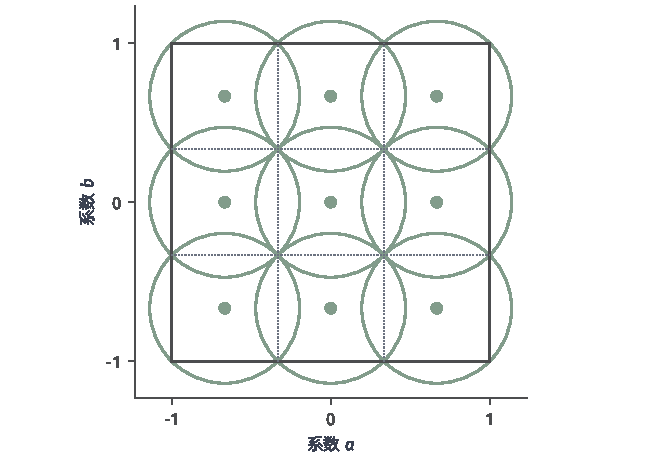
\includegraphics[width=112mm]{figures/00-shared/mathematical-preliminaries-upper/05-space-and-geometry/matplotlib/concepts-analysis-functional/covering-centers.pdf}
 \functionalinlinefigurecaption{fig:functional-covering-centers}
   {覆盖一个区域的几何图景。方形区域$[-1,1]^2$上，$9$个半径$\sqrt2/3$的圆盘中心排成$3\times3$网格$\{-2/3,0,2/3\}^2$；方形四角到最近中心的距离恰为$\sqrt2/3$，故整个方形被覆盖。代表数由区域在所选度量下的延伸和精度决定；正文对一维常值族给出显式估计$N\ge M/(2\delta)$。参数个数未变，区域尺度变大却使所需代表数增大。}
\end{minipage}
\end{center}

图~\ref{fig:functional-covering-centers}的系数平面并非抽象网格：它对应一元仿射函数类
\[
  f(t)=a+bt,\qquad (a,b)\in[-1,1]^2,\quad t\in[-1,1].
\]
两条仿射函数之差为$(a-a')+(b-b')t$，在上确界范数下的最大值在端点$t=\pm1$取得，等于$|a-a'|+|b-b'|$，即系数平面上的$\ell^1$距离（图中画欧氏圆盘只是几何示意；$\ell^1$球实为菱形）。把方形区域按精度$\delta$分块时，两个方向各需约$1/\delta$个中心，代表总数按$\delta^{-2}$增长；这与下一段一维常值族$N\ge M/(2\delta)$形成对照——代表数不仅随输出尺度$M$增大，还随参数维数与区域延伸增大。评价的始终是函数类在所选范数下的实际大小，而不是参数个数。

\paragraph{尺度与类的大小}

在非空输入域上取常值族
\[
  f_\theta(x)=M\theta,\qquad \theta\in[0,1],\quad M>0,
\]
使用上确界距离。一个代表常值函数$v$在半径$\delta$内所能覆盖的取值区间长度为$2\delta$（即$[v-\delta,v+\delta]$），而整个类的取值扫过$[0,M]$；要覆盖这个长度必须$N\cdot2\delta\ge M$，故
\[
  N(\delta,\mathcal F,d_\infty)\ge\frac{M}{2\delta}.
\]
参数数目没有变，输出尺度$M$却能使所需代表数增大。

对另一个常值族
\[
  f_\theta(x)=\sin(M\theta),\qquad \theta\in[0,2\pi],
\]
$M$为正整数，输出始终覆盖相同的$[-1,1]$，所以函数类本身没有随$M$扩大。参数导数可以变大，却不单独决定函数集合和覆盖数；这个对照说明应评价实际类，而不是只数参数或看参数化速度。

前面的折点目标可用多项式、样条或ReLU表示，回答的是单个函数的预算。若改问一整个类，就必须另外指定其范数半径、导数条件或其他约束，再在同一距离和精度下计算覆盖；不能由单例的精确表示取得全类的统一结论。

\paragraph{覆盖数与其他容量量的边界}

在后续学习理论中还会遇到两个容量量：伪维是在固定输入与阈值下检查哪些跨阈值模式可实现，胖打散还要求阈值两侧有指定间隔；覆盖数则累计给定距离下的近似代表数量。三者的评价对象与精度条件各不相同，不能从名称相近直接互换。谱有效维度依赖算子与惩罚尺度（见本章正则化参数极限一节），覆盖数依赖实际函数类及其距离；两者可以在额外定理下联系，却都不独自保证统计误差小、可识别或优化可解。相应学习结论留到后续学习理论中建立。

\subsection{查询树上的序贯覆盖数}
\label{subsubsec:sequential-covering}

\paragraph{从固定输入向量到查询树}

固定深度$T\ge1$的\term{查询树}
\[
  x_t:\{-1,1\}^{t-1}\to X,
\]
用$\sigma\in\{-1,1\}^{T}$表示一条分支路径。当前查询只依赖已有分支$\sigma_{<t}$，所以一个函数$f$在树上产生
\[
  f(x_t(\sigma_{<t}));
\]
这个对象有多个可能路径，不是一条预先固定的样本向量。

相应代表为实数树
\[
  v_t:\{-1,1\}^{t-1}\to\mathbb R.
\]
先固定一个有限树集合$\mathcal V$，再要求对每个$f\in\mathcal F$和每条$\sigma$，存在$v\in\mathcal V$使
\begin{equation}
  \left(\frac1T\sum_{t=1}^{T}
  \left|f(x_t(\sigma_{<t}))-v_t(\sigma_{<t})\right|^2\right)^{1/2}
  \le\delta.
  \label{eq:functional-sequential-cover}
\end{equation}
均方根只沿当前路径累计，代表树不必来自$\mathcal F$中的一个普通函数。

\paragraph{路径量词与最坏查询协议}

单独展开量词
\[
  \forall f\in\mathcal F\ \forall\sigma\in\{-1,1\}^T\ \exists v\in\mathcal V:
\]
有限树集合$\mathcal V$预先固定，所选代表树可随函数和路径改变。若改成“每个$f$先选一个代表并同时匹配所有路径”，就是更强的要求，不能把两种定义混用。

在给定查询树上取最小代表树数量，再对全部允许的深度$T$查询树取上确界，定义
\begin{equation}
  N_2^{\mathrm{seq}}(\delta,\mathcal F,T).
  \label{eq:functional-sequential-cover-number}
\end{equation}
这个上确界比较的是最坏查询协议，不是在路径上取随机平均；固定路径误差与“全部查询树最坏情形”是两个连续的定义步骤。例如两层树的根查询固定为$x_0$，第一次结果$\epsilon_1=-1$或$+1$后，第二次查询分别取$x_-$与$x_+$；代表树也要相应给出根处的$v_1$和两个第二层数值$v_2(-1)$、$v_2(+1)$。图~\ref{fig:functional-query-tree}用这个最小例子说明为什么不能用单个固定的两维样本向量替代树。这个定义只给组合容量，学习或预测保证另需具体任务和相应定理。

\begin{center}
\begin{minipage}{\linewidth}
 \centering
 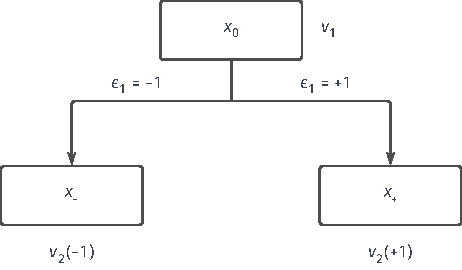
\includegraphics[width=78.281mm]{figures/00-shared/mathematical-preliminaries-upper/05-space-and-geometry/tikz/concepts-analysis-functional/query-tree.pdf}
 \functionalinlinefigurecaption{fig:functional-query-tree}
   {两层查询树。根查询$x_0$固定；第一次结果$\epsilon_1=-1$进入左支，第二次查询取$x_-$，结果$\epsilon_1=+1$进入右支，第二次查询取$x_+$。代表树在根处给$v_1$，在两个第二层结点分别给$v_2(-1)$与$v_2(+1)$。评价沿每条分支路径累计均方根误差，因此它不是一个固定两维样本向量，而是随历史变化的查询协议。}
\end{minipage}
\end{center}

\section{本章小结}
\label{sec:functional-summary}

\begin{enumerate}
  \item 把整个函数当作空间元素，必须先明确它是逐点函数还是几乎处处等价类，再选择误差、线性运算和完备性条件。Banach、Hilbert、$L^p$与核空间分别规定不同结构，不能当成彼此排斥的类别；同一底集或相同函数集合也不意味着误差口径相同。

  \item 弱导数通过测试恒等式保留变化信息，Sobolev范数同时控制函数与规定阶导数；它们不自动提供每点或边界读数。读取首先要良定义，随后才判断有界、代表唯一及位置变化；Riesz表示、RKHS和迹各有明确的输入、输出和条件。

  \item 正交展开、积分变换和积分方程分别记录方向、改变函数以及确定未知函数。闭性与完备性保障投影，正交系稠密保障范数展开，紧自伴和Mercer条件保障不同层次的谱结论；压缩迭代还要核对实际自映射和严格常数，不能只凭一个形式核公式取得全部结论。

  \item 函数拟合必须把数据、候选、目标和允许扰动同时给清。表示定理消去数据看不见的方向，具体二次结构才进一步给出有限系统和唯一函数；系数冗余、算法收敛、固定参数的数据稳定以及惩罚参数极限仍按各自变化量判断。积分变分先得到一阶弱条件，具体Poisson与热方程的解理论由后续微分方程章承接。

  \item 有限表示构造、已知函数的能量采样与整个函数类的覆盖数具有不同的近似对象。一个目标存在逼近器不保证找得到参数，能量值一致不保证最优解收敛，容量数量也不直接保证泛化；每一种判断都必须保留其误差、量词和条件。曲面弱微分（\term{Laplace--Beltrami算子}）、球面谱（\term{球谐函数}）、多尺度平滑（\term{尺度空间}）以及跨点搬运所需的几何结构，由流形章继续建立。
\end{enumerate}
